\PassOptionsToPackage{numbers}{natbib}
\documentclass{tufte-handout}
\usepackage{pgfplots}
\usepackage[dvipsnames]{xcolor}
\usepackage{amsmath, amssymb, amsthm}
\usepackage{mathtools}
\usepackage{bm}
\usepackage{thmtools}
\usepackage{enumitem}
\usepackage{tikz}
\usetikzlibrary{calc,arrows.meta,positioning,automata}
\usepackage{algorithm}
\usepackage{bbm}
\usepackage[normalem]{ulem}
\usepackage{listings}

% Color scheme
\definecolor{wp-bg}{HTML}{FDF6EF}
\definecolor{wp-text}{HTML}{2D1B0E}
\definecolor{wp-primary}{HTML}{C24A3A}
\definecolor{wp-accent}{HTML}{D4952E}
\definecolor{wp-light}{HTML}{F0DECA}
\definecolor{wp-muted}{HTML}{C4A88A}
\definecolor{wp-dark}{HTML}{1A0F07}
\definecolor{wp-code}{HTML}{FDF2E4}

\pagecolor{wp-bg}
\color{wp-text}
\hypersetup{colorlinks=true,linkcolor=wp-primary,urlcolor=wp-accent}

% Theorem environments
\declaretheorem[style=plain, name=Definition, numberwithin=section]{defn}
\declaretheorem[style=plain, name=Theorem, numberwithin=section]{thm}
\declaretheorem[style=plain, name=Lemma, numberwithin=section]{lem}
\declaretheorem[style=plain, name=Law, numberwithin=section]{law}
\declaretheorem[style=remark, name=Example, numberwithin=section]{exmp}
\declaretheorem[style=remark, name=Remark, numberwithin=section]{remark}
\declaretheorem[style=plain, name=Property, numberwithin=section]{prop}

\DeclareMathOperator*{\argmax}{argmax}
\DeclareMathOperator*{\argmin}{argmin}
\DeclareMathOperator{\E}{\mathbb{E}}
\DeclareMathOperator{\Var}{\mathbb{V}}
\DeclareMathOperator{\Cov}{\mathbb{C}\text{ov}}
\DeclareMathOperator{\KL}{KL}
\DeclareMathOperator{\Bern}{Bern}
\DeclareMathOperator{\Bin}{Bin}
\DeclareMathOperator{\Pois}{Pois}
\DeclareMathOperator{\Beta}{Beta}
\DeclareMathOperator{\Dir}{Dir}
\DeclareMathOperator{\Cat}{Cat}
\DeclareMathOperator{\Mult}{Mult}
\DeclareMathOperator{\Gam}{Gam}
\DeclareMathOperator{\N}{\mathcal{N}}
\DeclareMathOperator{\GP}{\mathcal{GP}}
\DeclareMathOperator{\IG}{IG}
\DeclareMathOperator{\Wish}{Wish}
\DeclareMathOperator{\InvWish}{InvWish}
\DeclareMathOperator{\ELBO}{ELBO}
\DeclareMathOperator{\tr}{tr}
\DeclareMathOperator{\sign}{sign}
\newcommand{\ind}{\mathbbm{1}}

\title{Do Acaso à Certeza\\ \large Probability Theory, Monte Carlo Methods, and the\\ Foundations of Machine Learning}
\author{Vitor N. Cabral de Oliveira}

\begin{document}

\maketitle

\begin{abstract}
    Esta obra traça a jornada intelectual que parte das primeiras indagações sobre o acaso ---
    jogos de azar, seguros, astronomia --- até a formulação matemática rigorosa da probabilidade,
    e desta até os algoritmos que hoje chamamos de aprendizado de máquina. Não se trata de uma
    coletânea de fórmulas justapostas, mas de uma narrativa lógica: cada conceito nasce de uma
    necessidade concreta, cada teorema resolve um problema que o precede.

    Começamos com a pergunta mais fundamental --- \textit{o que significa a probabilidade de um
    evento?} --- e, a partir dela, construímos todo o edifício. Cadeias de Markov surgem quando
    a independência se mostra insuficiente. Monte Carlo surge quando as integrais se mostram
    intratáveis. E aprendizado de máquina surge como a fusão natural de tudo isso: modelos
    probabilísticos de um mundo que nunca observamos completamente.
\end{abstract}

\newpage
\hypersetup{linkcolor=wp-text}
\tableofcontents
\hypersetup{linkcolor=wp-primary}

\newpage

%%%%%%%%%%%%%%%%%%%%%%%%%%%%%%%%%%%%%%%%%%%%%%%%%%%%%%%%%%%%%%%%%%%%%%%%%%%%%%%%
% PART I: FUNDAMENTOS DE PROBABILIDADE
%%%%%%%%%%%%%%%%%%%%%%%%%%%%%%%%%%%%%%%%%%%%%%%%%%%%%%%%%%%%%%%%%%%%%%%%%%%%%%%%

\part{Fundamentos de Probabilidade}

\section{O Nascimento da Probabilidade}

\paragraph{A Antiguidade e o Acaso}

Antes do século XVII, o acaso não era um objeto matemático --- era uma força misteriosa,
domínio dos deuses ou da fortuna. Os gregos antigos, apesar de seu extraordinário desenvolvimento
da geometria, nunca formalizaram o acaso. Aristóteles distinguia eventos que ocorrem
``sempre'', ``na maioria das vezes'' e ``por acaso'', mas não havia uma teoria do último.

Os romanos, por sua vez, eram ávidos jogadores. Lançavam ossos (astrágalos) e moedas em
rituais e apostas, mas novamente sem uma matematização. O dado de seis faces \textit{(tessera)}
era conhecido, mas ninguém havia perguntado: qual a probabilidade de obter um 7 com dois dados?

O que faltava não era inteligência, mas um conceito: o de \textbf{espaço amostral}.
Sem a noção de que todos os resultados possíveis formam um conjunto estruturado, a
probabilidade permanece uma intuição sem linguagem.

\paragraph{Gerolamo Cardano (1501--1576): O Primeiro Calculista}

Cardano foi médico, astrólogo e matemático --- e jogador inveterado. Em seu \textit{Liber de Ludo Aleae}
(O Livro dos Jogos de Azar), escrito por volta de 1564 mas publicado postumamente em 1663,
Cardano fez a primeira tentativa sistemática de calcular probabilidades.

Ele compreendeu o princípio fundamental: se um dado tem 6 faces igualmente prováveis, a
chance de obter uma face específica é $1/6$. Para eventos compostos, Cardano usava o que hoje
chamamos de \textbf{regra do produto} para eventos independentes e contagem de casos
favoráveis sobre casos possíveis. Ele sabia, por exemplo, que a probabilidade de obter pelo
menos um 1 em dois lançamentos é:

\[
P(\text{pelo menos um 1}) = 1 - P(\text{nenhum 1}) = 1 - \left(\frac{5}{6}\right)^2 = \frac{11}{36} \approx 0.306
\]

Esta já era uma aplicação implícita da \textbf{lei do complemento} e do conceito de
\textbf{independência}. No entanto, Cardano não formalizou esses princípios --- eram
ferramentas práticas para um jogador, não conceitos matemáticos abstratos.

\paragraph{Pascal e Fermat (1654): A Correspondência que Fundou a Probabilidade}

O verdadeiro nascimento da probabilidade como disciplina matemática ocorre em 1654,
numa troca de cartas entre Blaise Pascal (1623--1662) e Pierre de Fermat (1607--1665).
O problema que os motivou foi o \textbf{Problème des Partis} (Problema dos Pontos):

\begin{quote}
    Dois jogadores apostam igual valor numa série de rodadas justas. O primeiro a ganhar
    $n$ rodadas leva o prêmio total. O jogo é interrompido quando o jogador A tem $a$ vitórias
    e o jogador B tem $b$ vitórias ($a < n$, $b < n$). Como dividir o prêmio de forma justa?
\end{quote}

Pascal e Fermat chegaram independentemente à mesma solução: o prêmio deve ser dividido
proporcionalmente à probabilidade que cada jogador teria de vencer o jogo se ele continuasse.
Para calcular essas probabilidades, eles precisaram do que hoje chamamos de \textbf{triângulo de Pascal}
(conhecido anteriormente na China e Pérsia) e da \textbf{noção de valor esperado}.

Esta correspondência estabeleceu dois pilares:
\begin{enumerate}
    \item A probabilidade pode ser calculada \textit{a priori} por simetria (casos igualmente prováveis).
    \item A probabilidade de eventos futuros pode ser inferida de observações passadas.
\end{enumerate}

\paragraph{Jacob Bernoulli (1654--1705): A Lei dos Grandes Números}

Jacob Bernoulli (também chamado Jacques ou James) publicou postumamente sua obra-prima
\textit{Ars Conjectandi} (A Arte da Conjectura) em 1713, dividida em quatro partes:
\begin{enumerate}
    \item Reimpressão do \textit{Liber de Ludo Aleae} de Cardano.
    \item Teoria das permutações e combinações.
    \item Aplicação da probabilidade a problemas sociais e econômicos.
    \item O que ele chamou de \textit{``Teorema Dourado''} e hoje chamamos de
    \textbf{Lei (Fraca) dos Grandes Números}.
\end{enumerate}

O teorema de Bernoulli responde a uma questão fundamental: se observamos uma frequência
relativa em uma amostra, quão próximo isso está da probabilidade verdadeira?

\begin{thm}[Bernoulli, 1713]
    Seja $S_n$ o número de sucessos em $n$ tentativas independentes, cada uma com
    probabilidade $p$ de sucesso. Então, para qualquer $\varepsilon > 0$:
    \[
    \lim_{n \to \infty} P\left(\left|\frac{S_n}{n} - p\right| < \varepsilon\right) = 1
    \]
\end{thm}

Em palavras: a frequência relativa converge \textit{em probabilidade} para a probabilidade
verdadeira --- o que justifica, matematicamente, usar frequências observadas para estimar
probabilidades. Este teorema é o alicerce de toda a estatística frequentista.

Bernoulli derivou este resultado usando a distribuição binomial e limites superiores
(hoje diríamos: desigualdade de Chebyshev, que viria depois). Sua prova era tão complexa
que ele mesmo a chamou de ``nosso esforço digno de Hércules''.

\paragraph{De Moivre (1667--1754): A Curva Normal}

Abraham de Moivre, huguenote exilado na Inglaterra, descobriu em 1733 o que hoje chamamos
de \textbf{distribuição normal} como aproximação da binomial. Ele percebeu que os coeficientes
binomiais $C(n,k)$ para $n$ grande se aproximam de uma curva em forma de sino:

\[
C(n,k) p^k (1-p)^{n-k} \approx \frac{1}{\sqrt{2\pi np(1-p)}} \exp\left(-\frac{(k-np)^2}{2np(1-p)}\right)
\]

Esta foi a primeira versão do \textbf{Teorema Central do Limite}. De Moivre também cunhou
o termo \textbf{``curva normal''}, mas foi Gauss (mais de um século depois) quem a popularizou
na teoria dos erros de observação.

\paragraph{Thomas Bayes (1701--1761): Probabilidade Inversa}

O ensaio de Bayes, publicado postumamente em 1763 por Richard Price, introduziu o que hoje
chamamos de \textbf{Teorema de Bayes}. O problema de Bayes era: dada a frequência observada
de um evento, qual a probabilidade de que sua probabilidade intrínseca esteja num determinado
intervalo?

Bayes resolveu este problema (da ``probabilidade das causas'') usando o que hoje chamamos
de prior uniforme: assumindo nenhum conhecimento prévio sobre $p$ (a probabilidade de sucesso),
toda distribuição a priori é uniforme em $[0,1]$. A distribuição a posteriori de $p$ dado
$k$ sucessos em $n$ tentativas é:

\[
f(p \mid k, n) = \frac{(n+1)!}{k!(n-k)!} p^k (1-p)^{n-k}
\]

que hoje reconhecemos como uma distribuição Beta$(k+1, n-k+1)$.

Este resultado seminal plantou a semente de toda a inferência bayesiana, que veremos
em detalhe no Capítulo~\ref{sec:bayesian}.

\paragraph{Laplace (1749--1827): A Síntese}

Pierre-Simon Laplace consolidou todo o conhecimento probabilístico de seu tempo em sua
\textit{Théorie Analytique des Probabilités} (1812). Suas contribuições incluem:
\begin{itemize}
    \item A \textbf{definição clássica} de probabilidade: razão entre casos favoráveis e
    casos possíveis (igualmente prováveis).
    \item A \textbf{regra da sucessão}: a probabilidade de que o próximo evento seja um
    sucesso, dados $k$ sucessos em $n$ observações, é $(k+1)/(n+2)$.
    \item A generalização do Teorema Central do Limite.
    \item A aplicação da probabilidade à astronomia, meteorologia e jurisprudência.
\end{itemize}

A definição de Laplace, embora circular (``casos igualmente prováveis'' pressupõe o que
se quer definir), serviu como alicerce por quase um século.

\paragraph{O Problema da Definição: Século XIX}

A definição clássica de Laplace enfrentava problemas:
\begin{itemize}
    \item O que fazer com eventos não simétricos? (Ex: probabilidade de chuva)
    \item Como definir ``igualmente provável'' sem circularidade?
    \item Eventos com infinitos resultados possíveis (variáveis contínuas)?
\end{itemize}

Essas questões levaram ao desenvolvimento de duas escolas:
\begin{enumerate}
    \item \textbf{Frequentista} (Venn, von Mises): probabilidade é o limite da frequência
    relativa em infinitas repetições. Só faz sentido para eventos repetíveis.
    \item \textbf{Bayesiana} (Bayes, Laplace, de Finetti): probabilidade é um grau de
    crença, que pode ser atualizado por evidência via Teorema de Bayes. Aplica-se a
    qualquer evento incerto, mesmo único.
\end{enumerate}

A querela entre essas escolas persiste até hoje, e é fundamental para entender diferentes
abordagens em aprendizado de máquina.

\section{Os Axiomas de Kolmogorov}

\paragraph{A Necessidade de Rigor (1900--1933)}

No início do século XX, a teoria da probabilidade era um conjunto de resultados brilhantes,
mas sem fundamentação axiomática unificada. David Hilbert, em seus famosos problemas de 1900,
incluiu como sexto problema: ``Tratamento axiomático da probabilidade''.

Quem finalmente resolveu este problema foi o matemático soviético \textbf{Andrey Kolmogorov}
(1903--1987). Em seu livro \textit{Grundbegriffe der Wahrscheinlichkeitsrechnung}
(Fundamentos da Teoria da Probabilidade), de 1933, Kolmogorov apresentou um sistema de
axiomas que unifica e dá rigor a toda a disciplina.

A chave da abordagem de Kolmogorov foi conectar probabilidade à \textbf{teoria da medida},
desenvolvida por Lebesgue e Borel décadas antes. De repente, probabilidade não era mais
um ramo à parte --- era um caso especial da teoria da integração.

\paragraph{Espaços de Probabilidade}

\begin{defn}[Espaço de Probabilidade]
    Um espaço de probabilidade é uma tripla $(\Omega, \mathcal{F}, P)$, onde:
    \begin{enumerate}
        \item $\Omega$ é o \textbf{espaço amostral} --- o conjunto de todos os resultados
        possíveis de um experimento aleatório.
        \item $\mathcal{F}$ é uma $\sigma$-\textbf{álgebra} sobre $\Omega$ --- uma coleção
        de subconjuntos de $\Omega$ (chamados \textbf{eventos}) que satisfaz:
        \begin{itemize}
            \item $\Omega \in \mathcal{F}$.
            \item Se $A \in \mathcal{F}$, então $A^c = \Omega \setminus A \in \mathcal{F}$
            (fechamento sob complemento).
            \item Se $A_1, A_2, \dots \in \mathcal{F}$, então $\bigcup_{i=1}^\infty A_i \in \mathcal{F}$
            (fechamento sob uniões enumeráveis).
        \end{itemize}
        \item $P$ é uma \textbf{medida de probabilidade}: uma função $P: \mathcal{F} \to [0,1]$ tal que:
        \begin{itemize}
            \item $P(\Omega) = 1$.
            \item Para qualquer sequência enumerável de eventos disjuntos $A_1, A_2, \dots$,
            $P(\bigcup_{i=1}^\infty A_i) = \sum_{i=1}^\infty P(A_i)$ (aditividade enumerável).
        \end{itemize}
    \end{enumerate}
\end{defn}

A introdução da $\sigma$-álgebra não é mera neurose matemática. Ela resolve um problema
profundo: existem subconjuntos de $\mathbb{R}$ (ou $\mathbb{R}^n$) que são tão ``patológicos''
que não podemos atribuir-lhes uma medida de forma consistente. A $\sigma$-álgebra restringe
nossa atenção a conjuntos ``bem-comportados''.

Para a maioria das aplicações práticas e de aprendizado de máquina, podemos tomar $\Omega = \mathbb{R}^n$
e $\mathcal{F}$ como a $\sigma$-álgebra de Borel (gerada por intervalos abertos).

\paragraph{Propriedades Fundamentais}

Dos axiomas de Kolmogorov decorrem imediatamente propriedades essenciais:

\begin{prop}[Propriedades Básicas]
    Para qualquer espaço de probabilidade $(\Omega, \mathcal{F}, P)$ e eventos $A, B \in \mathcal{F}$:
    \begin{enumerate}
        \item $P(\emptyset) = 0$.
        \item $P(A^c) = 1 - P(A)$ (lei do complemento).
        \item Se $A \subseteq B$, então $P(A) \le P(B)$ (monotonicidade).
        \item $0 \le P(A) \le 1$.
        \item $P(A \cup B) = P(A) + P(B) - P(A \cap B)$ (regra da soma).
        \item $P(A \cup B) \le P(A) + P(B)$ (subaditividade).
    \end{enumerate}
\end{prop}

\begin{proof}
    \hfill
    \begin{enumerate}
        \item $\emptyset$ e $\Omega$ são disjuntos, e $\Omega = \Omega \cup \emptyset$.
        Pela aditividade: $P(\Omega) = P(\Omega) + P(\emptyset)$. Como $P(\Omega)=1$, segue que $P(\emptyset)=0$.
        \item $\Omega = A \cup A^c$, com $A$ e $A^c$ disjuntos. Logo $1 = P(A) + P(A^c)$.
        \item $B = A \cup (B \setminus A)$, união disjunta. Como $P(B \setminus A) \ge 0$, temos $P(B) \ge P(A)$.
        \item Segue de $0 = P(\emptyset) \le P(A) \le P(\Omega) = 1$.
        \item Escrevemos $A \cup B = A \cup (B \setminus (A \cap B))$, união disjunta.
        Então $P(A \cup B) = P(A) + P(B) - P(A \cap B)$.
        \item Segue da propriedade anterior, pois $P(A \cap B) \ge 0$.
    \end{enumerate}
\end{proof}

\subsection{Probabilidade Condicional e Independência}

\begin{defn}[Probabilidade Condicional]
    Sejam $A, B \in \mathcal{F}$ com $P(B) > 0$. A probabilidade condicional de $A$ dado $B$ é:
    \[
    P(A \mid B) = \frac{P(A \cap B)}{P(B)}
    \]
\end{defn}

A probabilidade condicional responde à pergunta: ``sabendo que $B$ ocorreu, qual a chance de $A$?''
Esta é a {\it atualização} de crenças diante de nova evidência --- o coração da inferência.

\begin{prop}[Regra do Produto]
    \[
    P(A \cap B) = P(A \mid B) P(B) = P(B \mid A) P(A)
    \]
\end{prop}

\begin{defn}[Independência]
    Dois eventos $A, B$ são \textbf{independentes} se:
    \[
    P(A \cap B) = P(A) P(B)
    \]
    Equivalentemente, $P(A \mid B) = P(A)$ e $P(B \mid A) = P(B)$.
\end{defn}

A independência é um dos conceitos mais importantes e mais mal compreendidos da probabilidade.
Ela não significa que eventos são ``não relacionados'' (há várias formas de relação), mas
sim que a ocorrência de um não altera a probabilidade do outro.

\begin{exmp}
    Lance uma moeda justa duas vezes. O evento $A = \text{``cara no primeiro lance''}$ e
    $B = \text{``cara no segundo lance''}$ são independentes. Mas $A$ e $C = \text{``mesmo
    resultado nos dois lances''}$ não são: $P(A \cap C) = 1/4 \neq P(A)P(C) = (1/2)(1/2) = 1/4$?
    Neste caso, são independentes! $P(C) = 1/2$, $P(A)P(C) = 1/4 = P(A \cap C)$.
\end{exmp}

A independência de eventos é uma propriedade matemática precisa, que nem sempre coincide
com a intuição de ``causalidade'' ou ``relação''.

\paragraph{Teorema de Bayes}

\begin{thm}[Bayes]
    Seja $\{A_1, A_2, \dots\}$ uma partição de $\Omega$ (eventos disjuntos cuja união é $\Omega$),
    com $P(A_i) > 0$ para todo $i$. Então, para qualquer evento $B$ com $P(B) > 0$:
    \[
    P(A_i \mid B) = \frac{P(B \mid A_i) P(A_i)}{\sum_j P(B \mid A_j) P(A_j)}
    \]
\end{thm}

O Teorema de Bayes é a regra de atualização ótima de crenças. Em aprendizado de máquina,
ele aparece toda vez que se deseja inferir parâmetros (causas) a partir de dados (efeitos):
\begin{align*}
    \underbrace{P(\theta \mid \mathcal{D})}_{\text{posterior}} &=
    \frac{\overbrace{P(\mathcal{D} \mid \theta)}^{\text{verossimilhança}} \overbrace{P(\theta)}^{\text{priori}}}
    {\underbrace{P(\mathcal{D})}_{\text{evidência}}}
\end{align*}

\begin{exmp}[Diagnóstico Médico]
    Uma doença afeta 1\% da população. Um teste detecta a doença com 99\% de acurácia
    (sensibilidade), mas tem 5\% de falsos positivos (especificidade de 95\%). Se uma pessoa
    testa positivo, qual a probabilidade de que ela realmente tenha a doença?

    Seja $D$ o evento ``ter a doença'' e $T$ o evento ``testar positivo''. Temos:
    \[
    P(D) = 0.01,\quad P(T\mid D) = 0.99,\quad P(T\mid D^c) = 0.05
    \]
    Pelo Teorema de Bayes:
    \[
    P(D\mid T) = \frac{0.99 \times 0.01}{0.99 \times 0.01 + 0.05 \times 0.99}
    = \frac{0.0099}{0.0099 + 0.0495} \approx 0.167
    \]
    Apenas 16.7\%! A intuição falha porque ignoramos a baixa prevalência. Este exemplo
    ilustra por que testes em massa precisam ser seguidos de confirmação.
\end{exmp}

\subsection{Variáveis Aleatórias}

\begin{defn}[Variável Aleatória]
    Uma \textbf{variável aleatória} $X$ é uma função mensurável $X: \Omega \to \mathbb{R}$.
    Isto é, para cada evento $B \subseteq \mathbb{R}$ (Borel), o conjunto
    $\{\omega \in \Omega : X(\omega) \in B\}$ pertence a $\mathcal{F}$.
\end{defn}

A mensurabilidade é o que nos permite transferir a medida de probabilidade de $\Omega$ para
$\mathbb{R}$: definimos $P(X \in B) = P(\{\omega : X(\omega) \in B\})$.

\begin{defn}[Função de Distribuição Acumulada (CDF)]
    A função de distribuição de $X$ é:
    \[
    F_X(x) = P(X \le x)
    \]
    Uma CDF satisfaz:
    \begin{enumerate}
        \item $\lim_{x\to -\infty} F_X(x) = 0$, $\lim_{x\to\infty} F_X(x) = 1$.
        \item $F_X$ é não-decrescente.
        \item $F_X$ é contínua à direita: $\lim_{y \to x^+} F_X(y) = F_X(x)$.
    \end{enumerate}
\end{defn}

\begin{defn}[PDF e PMF]
    \begin{itemize}
        \item Se $X$ é \textbf{discreta}, sua função de probabilidade (PMF) é
        $p_X(x) = P(X = x)$. A CDF é $F_X(x) = \sum_{t \le x} p_X(t)$.
        \item Se $X$ é \textbf{contínua}, sua função densidade de probabilidade (PDF)
        satisfaz $F_X(x) = \int_{-\infty}^x f_X(t)\,dt$, e $f_X(x) = F_X'(x)$.
    \end{itemize}
\end{defn}

\paragraph{Esperança e Momentos}

\begin{defn}[Valor Esperado]
    A esperança (ou média) de uma variável aleatória $X$ é:
    \[
    \E[X] = \begin{cases}
        \sum_{x} x\,p_X(x) & X \text{ discreta} \\[4pt]
        \int_{-\infty}^\infty x\,f_X(x)\,dx & X \text{ contínua}
    \end{cases}
    \]
    Desde que a soma/integral convirja absolutamente.
\end{defn}

O valor esperado pode ser pensado como o ``centro de massa'' da distribuição. A operador
$\E$ é \textbf{linear}: $\E[aX+b] = a\E[X] + b$.

\begin{defn}[Variância]
    \[
    \Var(X) = \E[(X - \E[X])^2] = \E[X^2] - \E[X]^2
    \]
    O desvio padrão é $\sigma_X = \sqrt{\Var(X)}$.
\end{defn}

A variância mede a dispersão da distribuição em torno da média. Quanto maior, mais
``espalhada'' a distribuição.

\begin{defn}[Momentos]
    O $k$-ésimo momento de $X$ é $\E[X^k]$.
    O $k$-ésimo momento central é $\E[(X - \E[X])^k]$.
    O terceiro momento central mede \textbf{assimetria} (skewness), e o quarto mede
    \textbf{curtose} (achatamento).
\end{defn}

\subsection{Lei dos Grandes Números}

A Lei dos Grandes Números é, possivelmente, o teorema mais importante da probabilidade,
pois conecta o mundo abstrato das probabilidades ao mundo concreto das frequências.

\paragraph{Desigualdade de Chebyshev}

Antes de provarmos a lei, precisamos de uma ferramenta:

\begin{lem}[Desigualdade de Markov]
    Se $X \ge 0$, então para qualquer $t > 0$:
    \[
    P(X \ge t) \le \frac{\E[X]}{t}
    \]
\end{lem}

\begin{proof}
    $\E[X] = \int_0^\infty x f_X(x) dx \ge \int_t^\infty x f_X(x) dx \ge t \int_t^\infty f_X(x) dx = t P(X \ge t)$.
\end{proof}

\begin{lem}[Desigualdade de Chebyshev]
    Para qualquer variável aleatória $X$ com média $\mu$ e variância $\sigma^2$:
    \[
    P(|X - \mu| \ge \varepsilon) \le \frac{\sigma^2}{\varepsilon^2}
    \]
\end{lem}

\begin{proof}
    Aplicamos Markov à variável $Y = (X-\mu)^2 \ge 0$:
    $P(|X-\mu| \ge \varepsilon) = P(Y \ge \varepsilon^2) \le \E[Y]/\varepsilon^2 = \sigma^2/\varepsilon^2$.
\end{proof}

Chebyshev nos dá uma cota superior para a probabilidade de que uma variável aleatória
se desvie de sua média. A desigualdade é surpreendentemente geral --- não assume nenhuma
distribuição específica --- mas por isso mesmo é conservadora.

\begin{thm}[Lei Fraca dos Grandes Números]
    Sejam $X_1, X_2, \dots$ variáveis aleatórias i.i.d. (independentes e identicamente
    distribuídas) com média $\mu$ e variância finita $\sigma^2$. Então, para qualquer
    $\varepsilon > 0$:
    \[
    \lim_{n \to \infty} P\left(\left|\frac{1}{n}\sum_{i=1}^n X_i - \mu\right| < \varepsilon\right) = 1
    \]
\end{thm}

\begin{proof}
    Seja $\bar{X}_n = \frac{1}{n}\sum_{i=1}^n X_i$. Pela linearidade, $\E[\bar{X}_n] = \mu$.
    Pela independência, $\Var(\bar{X}_n) = \sigma^2/n$. Por Chebyshev:
    \[
    P(|\bar{X}_n - \mu| \ge \varepsilon) \le \frac{\sigma^2}{n\varepsilon^2} \to 0
    \]
\end{proof}

Esta é a versão ``fraca'' (convergência em probabilidade). Existe também a versão
``forte'' (convergência quase certa), provada por Kolmogorov, que estabelece que
$\bar{X}_n \to \mu$ com probabilidade 1.

\paragraph{Significado para o Aprendizado de Máquina}

A Lei dos Grandes Números é a justificativa matemática para o aprendizado a partir de dados:

\begin{enumerate}
    \item O erro empírico $\frac{1}{n}\sum \ell(y_i, f(x_i))$ converge para o erro esperado
    $\E[\ell(Y, f(X))]$ --- desde que os dados sejam i.i.d.
    \item A frequência relativa de um evento converge para sua probabilidade --- justificando
    estimativas frequentistas.
    \item A média amostral converge para a média populacional --- base da estatística descritiva.
\end{enumerate}

A suposição i.i.d. (independent and identically distributed) é onipresente em ML, mas
frequentemente violada na prática (dados de séries temporais, dados não-estacionários).
Compreender as consequências dessas violações é uma marca da maturidade técnica.

\subsection{Teorema Central do Limite}

Se a Lei dos Grandes Números nos diz a \textit{média} converge, o Teorema Central do
Limite (TCL) nos diz \textit{como} ela converge.

\begin{thm}[Teorema Central do Limite --- Lindeberg--Lévy]
    Sejam $X_1, X_2, \dots$ variáveis i.i.d. com média $\mu$ e variância $\sigma^2 < \infty$.
    Então:
    \[
    \sqrt{n}\left(\frac{1}{n}\sum_{i=1}^n X_i - \mu\right) \xrightarrow{d} \mathcal{N}(0, \sigma^2)
    \]
    Ou seja, a distribuição da média amostral padronizada converge para a normal padrão.
\end{thm}

O TCL é notável por sua universalidade: \textit{qualquer} distribuição com variância finita,
quando somada repetidamente, produz uma distribuição aproximadamente normal. Isto explica
por que a distribuição normal aparece tão frequentemente na natureza --- desde erros de
medição até alturas de populações.

\begin{exmp}
    Considere $X_i \sim \Bern(p)$ (Bernoulli). A soma $S_n = \sum X_i \sim \Bin(n, p)$.
    Pelo TCL, para $n$ grande:
    \[
    \frac{S_n - np}{\sqrt{np(1-p)}} \approx \mathcal{N}(0, 1)
    \]
    Esta aproximação é a base de testes de hipótese para proporções e do intervalo de
    confiança de Wald.
\end{exmp}

Para o aprendizado de máquina, o TCL tem implicações profundas:
\begin{itemize}
    \item O erro de generalização (diferença entre erro de teste e erro esperado) é
    aproximadamente normal, permitindo intervalos de confiança.
    \item Estimadores de máxima verossimilhança (MLE) são assintoticamente normais.
    \item A inicialização aleatória de pesos em redes neurais, somada ao TCL, justifica
    a inicialização de Xavier/Glorot.
\end{itemize}

\section{Pensamento Frequentista vs. Bayesiano}

\paragraph{A Escola Frequentista}

Para o frequentista, probabilidade é uma propriedade objetiva do mundo, definida como
o limite da frequência relativa em repetições infinitas. Parâmetros são fixos
(embora desconhecidos), e os dados são aleatórios.

\textbf{Representantes}: Venn, von Mises, Neyman, Pearson, Fisher (em parte).

\textbf{Princípios}:
\begin{itemize}
    \item Hipóteses são testadas (aceitas ou rejeitadas) com base em dados.
    \item Intervalos de confiança contêm o parâmetro verdadeiro com determinada
    frequência em repetições hipotéticas.
    \item O p-valor mede a compatibilidade dos dados com a hipótese nula.
    \item Não se atribuem probabilidades a parâmetros (eles não são aleatórios).
\end{itemize}

\textbf{Exemplo}: Um intervalo de confiança de 95\% para a média:
\[
\bar{x} \pm 1.96 \frac{\sigma}{\sqrt{n}}
\]
significa: ``se repetíssemos este experimento muitas vezes, 95\% dos intervalos conteriam
a média verdadeira'' --- não que há 95\% de chance de a média estar no intervalo.

\paragraph{A Escola Bayesiana}

Para o bayesiano, probabilidade é um grau de crença subjetivo, que pode (e deve) ser
atualizado à luz de nova evidência. Parâmetros são aleatórios (no sentido de que nossa
incerteza sobre eles é descrita por uma distribuição), e os dados são fixos
(uma vez observados).

\textbf{Representantes}: Bayes, Laplace, de Finetti, Jeffreys, Savage, Lindley.

\textbf{Princípios}:
\begin{itemize}
    \item A incerteza sobre parâmetros é quantificada por uma distribuição a priori $P(\theta)$.
    \item Os dados atualizam esta crença via Teorema de Bayes: $P(\theta \mid \mathcal{D}) \propto P(\mathcal{D} \mid \theta) P(\theta)$.
    \item Toda inferência é baseada na distribuição a posteriori.
    \item Não há distinção fundamental entre parâmetros e dados --- tudo é modelado probabilisticamente.
\end{itemize}

\textbf{Exemplo}: Um intervalo de credibilidade de 95\% é o intervalo $[a, b]$ tal que
$P(a \le \theta \le b \mid \mathcal{D}) = 0.95$. Isto \textit{é} uma afirmação
probabilística sobre $\theta$, condicionada nos dados.

\paragraph{Impacto no Aprendizado de Máquina}

Ambas as escolas influenciaram profundamente o ML:

\begin{marginfigure}
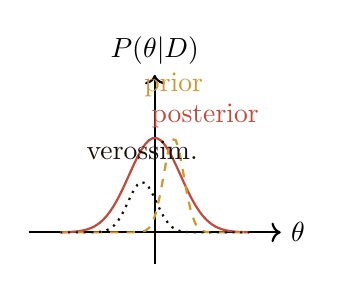
\begin{tikzpicture}[scale=0.8]
\draw[thick,->] (-2,0) -- (2,0) node[right] {$\theta$};
\draw[thick,->] (0,-0.5) -- (0,2.5) node[above] {$P(\theta|D)$};
\draw[wp-primary, thick, domain=-1.5:1.5, samples=50] plot (\x, {1.5*exp(-3*\x*\x)});
\draw[wp-accent, thick, dashed, domain=-1.5:1.5, samples=50] plot (\x, {1.5*exp(-20*(\x-0.3)*(\x-0.3))});
\draw[wp-dark, thick, dotted, domain=-1.5:1.5, samples=50] plot (\x, {0.8*exp(-10*(\x+0.2)*(\x+0.2))});
\node[wp-primary, above] at (0.8, 1.5) {posterior};
\node[wp-accent, above] at (0.3, 2.0) {prior};
\node[wp-dark, above] at (-0.2, 1.0) {verossim.};
\end{tikzpicture}
\caption{Relação entre prior, verossimilhança e posterior no Teorema de Bayes.}
\end{marginfigure}

\begin{enumerate}
    \item \textbf{Regularização}: A regularização $L_2$ (weight decay) corresponde a uma
    priori Gaussiana nos pesos. A regularização $L_1$ (Lasso) corresponde a uma priori
    Laplace. A escolha da regularização é uma escolha bayesiana implícita.
    \item \textbf{Dropout}: O dropout pode ser interpretado como uma aproximação
    bayesiana variacional (Gal \& Ghahramani, 2016).
    \item \textbf{Bayesian Neural Networks}: Redes neurais bayesianas mantêm uma
    distribuição sobre os pesos, quantificando incerteza nas previsões.
    \item \textbf{Model Selection}: A evidência marginal $P(\mathcal{D})$ (verossimilhança
    integrada sobre a priori) é usada para comparar modelos.
\end{enumerate}

O debate frequentista vs. bayesiano em ML frequentemente se resolve de forma pragmática:
usa-se o que funciona. Mas compreender ambas as perspectivas é essencial para ler a literatura,
interpretar resultados e evitar armadilhas conceituais.

%%%%%%%%%%%%%%%%%%%%%%%%%%%%%%%%%%%%%%%%%%%%%%%%%%%%%%%%%%%%%%%%%%%%%%%%%%%%%%%%
% PART II: CADEIAS DE MARKOV
%%%%%%%%%%%%%%%%%%%%%%%%%%%%%%%%%%%%%%%%%%%%%%%%%%%%%%%%%%%%%%%%%%%%%%%%%%%%%%%%

\part{Cadeias de Markov}

\section{A quebra da Independência}

\paragraph{O Contexto: O Mundo Não É Independente}

Até o final do século XIX, a teoria da probabilidade estava firmemente ancorada no conceito
de independência. A Lei dos Grandes Números de Bernoulli, o Teorema Central do Limite de
De Moivre--Laplace --- todos assumiam observações independentes.

Mas o mundo real desafia esta suposição. A temperatura de amanhã não é independente da
temperatura de hoje. A próxima palavra em uma frase não é independente da anterior.
O preço de uma ação amanhã depende do preço de hoje.

\begin{exmp}[A Falácia da Independência]
    Suponha que modelemos o clima como independente entre dias: a probabilidade de chuva
    hoje é $p$, independente do que ocorreu ontem. Este modelo tem duas consequências absurdas:
    \begin{enumerate}
        \item O tempo de permanência em um estado (dias consecutivos de chuva) segue uma
        distribuição geométrica, que decai exponencialmente. Na realidade, sistemas climáticos
        têm ``memória'' de dias ou semanas.
        \item A previsão para amanhã ignora toda a história recente --- um meteorologista
        que visse 5 dias consecutivos de chuva daria a mesma previsão que um que visse 5 dias
        de sol.
    \end{enumerate}
\end{exmp}

O que precisamos é de um modelo que capture dependência temporal sem exigir a memória
completa de todo o passado.

\paragraph{Andrey Markov (1856--1922): O Rebelde}

Andrey Andreyevich Markov foi um matemático russo, aluno de Chebyshev e membro da
Academia de Ciências de São Petersburgo. Discípulo da escola de Chebyshev (que também
produziu Lyapunov), Markov era conhecido por seu temperamento forte e suas convicções
políticas liberais (numa época em que isso era perigoso na Rússia czarista).

Em 1906, Markov publicou um artigo que desafiava a suposição de independência predominante.
Sua motivação era tanto matemática quanto filosófica: ele acreditava que a probabilidade
deveria ser capaz de modelar fenômenos dependentes, e que os teoremas limite deveriam
valer para sequências dependentes também.

Markov escolheu um objeto de estudo curioso: as 20.000 letras do poema \textit{Eugene Onegin}
de Pushkin. Ele sequenciou as vogais e consoantes do texto e perguntou: a probabilidade de
uma letra ser vogal depende da letra anterior?

\begin{exmp}[O Experimento de Markov com Eugene Onegin]
    Markov contou as transições entre vogais (V) e consoantes (C) no texto de Pushkin.
    Ele encontrou:
    \begin{align*}
        P(\text{próxima letra} = V \mid \text{atual} = V) &= 0.128 \\
        P(\text{próxima letra} = V \mid \text{atual} = C) &= 0.337
    \end{align*}
    Se as letras fossem independentes, a probabilidade de uma letra ser vogal seria a mesma
    (~0.432), independente da letra anterior. Os dados de Markov mostram claramente que
    não são independentes: uma vogal tende a ser seguida por uma consoante.
\end{exmp}

Este experimento é considerado o nascimento das cadeias de Markov.

\subsection{Definição e Propriedades}

\begin{defn}[Processo Estocástico]
    Um \textbf{processo estocástico} é uma coleção de variáveis aleatórias
    $\{X_t : t \in \mathcal{T}\}$ indexadas por um conjunto $\mathcal{T}$ (geralmente
    o tempo). Se $\mathcal{T}$ é discreto ($t = 0, 1, 2, \dots$), temos um
    \textbf{processo em tempo discreto}.
\end{defn}

\begin{defn}[Propriedade de Markov]
    Um processo estocástico $\{X_t\}$ em tempo discreto satisfaz a \textbf{propriedade de Markov}
    se, para todo $t \ge 1$ e todos os estados $x_0, \dots, x_t$:
    \[
    P(X_t = x_t \mid X_{t-1} = x_{t-1}, X_{t-2} = x_{t-2}, \dots, X_0 = x_0)
    = P(X_t = x_t \mid X_{t-1} = x_{t-1})
    \]
\end{defn}

A propriedade de Markov estabelece que: dado o presente, o futuro é independente do passado.
Esta é a forma mais simples de dependência temporal --- uma memória de apenas um passo.
Apesar de sua simplicidade, ela captura uma enorme gama de fenômenos.

\begin{defn}[Cadeia de Markov em Tempo Discreto]
    Uma \textbf{cadeia de Markov} é um processo estocástico $\{X_t\}_{t=0}^\infty$ com:
    \begin{enumerate}
        \item Um conjunto (finito ou enumerável) de \textbf{estados} $\mathcal{S}$.
        \item A propriedade de Markov:
        \[
        P(X_t = j \mid X_{t-1} = i, X_{t-2}, \dots) = P(X_t = j \mid X_{t-1} = i) = p_{ij}(t)
        \]
        \item Se as probabilidades de transição não dependem do tempo $t$ (\textbf{homogeneidade temporal}):
        \[
        P(X_t = j \mid X_{t-1} = i) = p_{ij}
        \]
    \end{enumerate}
\end{defn}

\paragraph{Matriz de Transição}

Para uma cadeia de Markov homogênea com estados $\{1, 2, \dots, m\}$, a \textbf{matriz de transição}
$P$ é uma matriz $m \times m$ onde:
\[
P_{ij} = p_{ij} = P(X_t = j \mid X_{t-1} = i)
\]

A matriz $P$ é \textbf{estocástica} (cada linha soma 1):
\[
\sum_{j=1}^m P_{ij} = 1 \quad \forall i
\]

\begin{marginfigure}
\centering
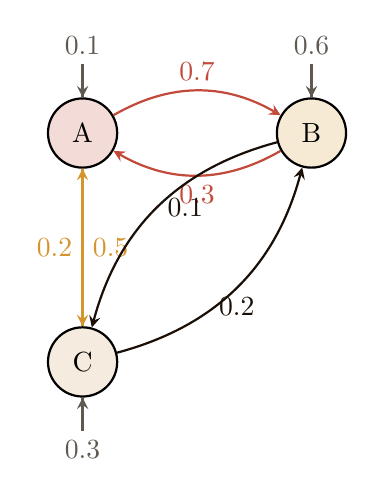
\begin{tikzpicture}[>=stealth, node distance=2cm, thick]
\node[state, draw, circle, fill=wp-primary!20] (A) {A};
\node[state, draw, circle, fill=wp-accent!20, right=of A] (B) {B};
\node[state, draw, circle, fill=wp-light!60, below=of A] (C) {C};
\draw[->, wp-primary] (A) to[bend left] node[midway,above] {$0.7$} (B);
\draw[->, wp-primary] (B) to[bend left] node[midway,below] {$0.3$} (A);
\draw[->, wp-accent] (A) -- node[midway,left] {$0.2$} (C);
\draw[->, wp-accent] (C) -- node[midway,right] {$0.5$} (A);
\draw[->, wp-dark] (B) to[bend right] node[midway,right] {$0.1$} (C);
\draw[->, wp-dark] (C) to[bend right] node[midway,below] {$0.2$} (B);
\draw[->, wp-light!40!black] (A) .. controls +(90:1cm) and +(90:1cm) .. node[midway,above] {$0.1$} (A);
\draw[->, wp-light!40!black] (B) .. controls +(90:1cm) and +(90:1cm) .. node[midway,above] {$0.6$} (B);
\draw[->, wp-light!40!black] (C) .. controls +(270:1cm) and +(270:1cm) .. node[midway,below] {$0.3$} (C);
\end{tikzpicture}
\caption{Exemplo de cadeia de Markov com 3 estados e probabilidades de transição.}
\label{fig:markov_chain}
\end{marginfigure}

\paragraph{Distribuição Inicial e Evolução Temporal}

A cadeia é completamente especificada por:
\begin{enumerate}
    \item A \textbf{distribuição inicial}: $\pi^{(0)} = (\pi_1^{(0)}, \pi_2^{(0)}, \dots)$,
    onde $\pi_i^{(0)} = P(X_0 = i)$.
    \item A \textbf{matriz de transição} $P$.
\end{enumerate}

A distribuição após $t$ passos é:
\[
\pi^{(t)} = \pi^{(0)} P^t
\]
onde $\pi^{(t)}_j = P(X_t = j)$.

A transição em $k$ passos é dada por $P^k$ (a $k$-ésima potência da matriz de transição):
\[
P^k_{ij} = P(X_{t+k} = j \mid X_t = i)
\]

\begin{prop}[Equação de Chapman--Kolmogorov]
    Para quaisquer $m, n \ge 0$:
    \[
    P^{m+n} = P^m P^n
    \]
    Ou em componentes:
    \[
    P^{m+n}_{ij} = \sum_{k} P^m_{ik} P^n_{kj}
    \]
\end{prop}

\subsection{Classificação de Estados}

\begin{defn}[Acessibilidade e Comunicação]
    \begin{itemize}
        \item O estado $j$ é \textbf{acessível} de $i$ (denotado $i \to j$) se existe $t \ge 0$
        tal que $P^t_{ij} > 0$.
        \item Os estados $i$ e $j$ \textbf{comunicam-se} ($i \leftrightarrow j$) se $i \to j$
        e $j \to i$.
    \end{itemize}
    A relação de comunicação é uma relação de equivalência, particionando o espaço de
    estados em \textbf{classes de comunicação}.
\end{defn}

\begin{defn}[Classificação]
    Um estado $i$ é:
    \begin{itemize}
        \item \textbf{Recorrente} se $P_i(T_i < \infty) = 1$, onde $T_i = \min\{t \ge 1 : X_t = i\}$
        (tempo de primeiro retorno). A cadeia retorna a $i$ com probabilidade 1.
        \item \textbf{Transiente} se $P_i(T_i < \infty) < 1$. Existe probabilidade positiva
        de nunca retornar.
        \item \textbf{Absorvente} se $p_{ii} = 1$: uma vez lá, nunca sai.
        \item \textbf{Periódico} com período $d$ se $d = \gcd\{t > 0 : P^t_{ii} > 0\}$.
        Se $d = 1$, o estado é \textbf{aperiódico}.
    \end{itemize}
\end{defn}

\begin{defn}[Irredutibilidade]
    Uma cadeia de Markov é \textbf{irredutível} se todos os estados comunicam-se entre si
    (há apenas uma classe de comunicação).
\end{defn}

\subsection{Distribuição Estacionária}

\begin{defn}[Distribuição Estacionária]
    Uma distribuição de probabilidade $\pi = (\pi_1, \pi_2, \dots)$ sobre $\mathcal{S}$
    é \textbf{estacionária} (ou invariante) se:
    \[
    \pi = \pi P
    \]
    Isto é, $\pi_j = \sum_i \pi_i P_{ij}$ para todo $j$.
\end{defn}

Uma distribuição estacionária é um ponto fixo da dinâmica: se $X_t \sim \pi$, então
$X_{t+1} \sim \pi$. A cadeia ``esqueceu'' suas condições iniciais e estabilizou-se.

\begin{thm}[Existência e Unicidade]
    Para uma cadeia de Markov finita e irredutível:
    \begin{enumerate}
        \item Existe uma única distribuição estacionária $\pi$.
        \item $\pi_i > 0$ para todo $i$.
        \item $\pi_i = 1/\E_i[T_i]$, onde $\E_i[T_i]$ é o tempo esperado de retorno a $i$.
    \end{enumerate}
\end{thm}

\begin{thm}[Convergência para o Equilíbrio]
    Se a cadeia é irredutível e aperiódica, então para qualquer distribuição inicial $\pi^{(0)}$:
    \[
    \lim_{t \to \infty} \pi^{(t)} = \pi
    \]
    onde $\pi$ é a distribuição estacionária. Mais ainda, a convergência é exponencial
    (em termos da distância de variação total).
\end{thm}

\begin{exmp}[Meteorologia Simplificada]
    Considere um modelo de clima com 2 estados: $\mathcal{S} = \{S, C\}$ (sol e chuva).
    A matriz de transição:
    \[
    P = \begin{pmatrix}
    0.9 & 0.1 \\
    0.5 & 0.5
    \end{pmatrix}
    \]
    Isto significa: $P(\text{sol amanhã} \mid \text{sol hoje}) = 0.9$,
    $P(\text{chuva amanhã} \mid \text{sol hoje}) = 0.1$,
    $P(\text{sol amanhã} \mid \text{chuva hoje}) = 0.5$,
    $P(\text{chuva amanhã} \mid \text{chuva hoje}) = 0.5$.

    A distribuição estacionária satisfaz $\pi = \pi P$:
    \begin{align*}
        \pi_S &= 0.9\pi_S + 0.5\pi_C \\
        \pi_C &= 0.1\pi_S + 0.5\pi_C \\
        \pi_S + \pi_C &= 1
    \end{align*}
    Resolvendo: $\pi_S = 5/6 \approx 0.833$, $\pi_C = 1/6 \approx 0.167$.
    A longo prazo, cerca de 83\% dos dias são de sol, independente do clima inicial.
\end{exmp}

\subsection{Balanço Detalhado e Reversibilidade}

\begin{defn}[Balanço Detalhado]
    Uma cadeia de Markov satisfaz a \textbf{condição de balanço detalhado} se existe
    uma distribuição $\pi$ tal que:
    \[
    \pi_i P_{ij} = \pi_j P_{ji} \quad \forall i, j
    \]
\end{defn}

Quando o balanço detalhado vale, a cadeia é dita \textbf{reversível}: a dinâmica parece
a mesma quando o tempo é invertido. Isto tem implicações profundas para algoritmos MCMC.

\begin{prop}
    Se o balanço detalhado vale para $\pi$, então $\pi$ é uma distribuição estacionária.
\end{prop}

\begin{proof}
    $\sum_i \pi_i P_{ij} = \sum_i \pi_j P_{ji} = \pi_j \sum_i P_{ji} = \pi_j$.
\end{proof}

O balanço detalhado é uma condição mais forte que a estacionariedade. Muitos algoritmos
MCMC (como Metropolis--Hastings) são construídos para garantir o balanço detalhado,
assegurando que a distribuição-alvo seja estacionária.

\section{Conceitos Avançados}

\paragraph{Cadeias de Markov em Espaços Contínuos}

Para variáveis contínuas, a matriz de transição é substituída por um \textbf{núcleo de transição}
$K(x, A) = P(X_{t+1} \in A \mid X_t = x)$. A distribuição estacionária satisfaz:
\[
\pi(A) = \int K(x, A) \pi(dx)
\]

O balanço detalhado torna-se:
\[
\pi(x) K(x, y) = \pi(y) K(y, x)
\]
onde $K(x, y)$ é a densidade de transição.

\paragraph{Cadeias de Markov em Aprendizado de Máquina}

As cadeias de Markov aparecem em múltiplos contextos em ML:

\begin{enumerate}
    \item \textbf{Modelagem de sequências}: Modelos de linguagem (n-gramas são cadeias de
    Markov de ordem $n-1$), Hidden Markov Models (HMMs) para reconhecimento de fala e
    bioinformática.
    \item \textbf{MCMC}: Algoritmos de Markov Chain Monte Carlo para inferência em modelos
    complexos (ver Capítulo~\ref{sec:mcmc}).
    \item \textbf{Aprendizado por Reforço}: Processos de Decisão de Markov (MDPs) são a
    base formal do RL.
    \item \textbf{Redes Neurais Recorrentes}: RNNs podem ser vistas como cadeias de Markov
    com estado oculto de alta dimensão.
    \item \textbf{Modelos de Difusão}: A fase forward de modelos de difusão é uma cadeia
    de Markov que adiciona ruído gaussiano aos dados.
\end{enumerate}

%%%%%%%%%%%%%%%%%%%%%%%%%%%%%%%%%%%%%%%%%%%%%%%%%%%%%%%%%%%%%%%%%%%%%%%%%%%%%%%%
% PART III: MONTE CARLO
%%%%%%%%%%%%%%%%%%%%%%%%%%%%%%%%%%%%%%%%%%%%%%%%%%%%%%%%%%%%%%%%%%%%%%%%%%%%%%%%

\part{Métodos de Monte Carlo}

\section{As Origens: Von Neumann, Ulam e a Bomba Atômica}

\paragraph{O Contexto: Los Alamos, 1940}

A história dos métodos de Monte Carlo começa no Projeto Manhattan, em Los Alamos,
Novo México. Os físicos Stanislaw Ulam, John von Neumann, Nicholas Metropolis e
Enrico Fermi enfrentavam um problema intratável: calcular o comportamento de nêutrons
em materiais fissionáveis.

As equações de transporte de nêutrons eram integrais multidimensionais complexas,
impossíveis de resolver analiticamente. Métodos numéricos tradicionais (diferenças finitas)
exigiam aproximações grosseiras ou esforço computacional inviável para a época.

\paragraph{A Ideia de Ulam}

Conta-se que Ulam, durante uma convalescença, tentava calcular a probabilidade de
conseguir uma determinada mão no jogo de paciência (Canfield). Após tentativas
combinatórias exaustivas, ele pensou: ``Em vez de calcular exatamente, por que não
jogar 100 partidas e contar quantas vezes a mão aparece?''

Esta intuição --- usar amostragem aleatória para estimar quantidades determinísticas ---
é a essência do método de Monte Carlo.

Ulam compartilhou a ideia com von Neumann, que imediatamente reconheceu seu potencial
para o problema de nêutrons. Von Neumann implementou o primeiro algoritmo de Monte Carlo
no computador ENIAC em 1947. Metropolis batizou o método de ``Monte Carlo'' em referência
ao cassino de Mônaco, terra do acaso.

\paragraph{O Problema Fundamental}

Suponha que queremos calcular:
\[
I = \int_a^b f(x) dx
\]
Se $f$ é simples, usamos o Teorema Fundamental do Cálculo. Mas em problemas reais,
$f$ pode ser uma função complicada de 10, 100 ou 1000 variáveis, sem primitiva conhecida.

A ideia de Monte Carlo é rewritar a integral como um valor esperado:
\[
I = \int_a^b f(x) dx = (b-a) \int_a^b f(x) \frac{1}{b-a} dx = (b-a) \E[f(X)]
\]
onde $X \sim \text{Uniforme}(a, b)$. Agora, pela Lei dos Grandes Números:
\[
\hat{I}_n = \frac{b-a}{n} \sum_{i=1}^n f(X_i) \xrightarrow{n\to\infty} I
\]
com $X_i$ i.i.d. $\text{Uniforme}(a, b)$.

Esta é a forma mais simples de Monte Carlo: estimar uma integral amostrando pontos
aleatórios e calculando a média de $f$ nestes pontos.

\subsection{Monte Carlo Clássico}

\begin{defn}[Estimador de Monte Carlo]
    Seja $X_1, \dots, X_n$ uma amostra i.i.d. de $X$ com distribuição $p(x)$.
    O estimador de Monte Carlo para $\E[f(X)]$ é:
    \[
    \hat{\mu}_n = \frac{1}{n} \sum_{i=1}^n f(X_i)
    \]
\end{defn}

\begin{prop}[Propriedades do Estimador MC]
    \begin{enumerate}
        \item \textbf{Não-viesado}: $\E[\hat{\mu}_n] = \E[f(X)]$.
        \item \textbf{Consistente}: Se $\Var(f(X)) < \infty$, então $\hat{\mu}_n \xrightarrow{P} \E[f(X)]$.
        \item \textbf{Erro padrão}: $\Var(\hat{\mu}_n) = \frac{\Var(f(X))}{n}$,
        então $\text{SE}(\hat{\mu}_n) = \frac{\sigma_f}{\sqrt{n}}$.
        \item \textbf{Normalidade assintótica}: $\frac{\hat{\mu}_n - \E[f(X)]}{\sigma_f/\sqrt{n}} \xrightarrow{d} \mathcal{N}(0, 1)$.
    \end{enumerate}
\end{prop}

Uma propriedade crucial: o erro de Monte Carlo decai como $O(1/\sqrt{n})$,
\textit{independentemente da dimensão do problema}! Isto contrasta com métodos de
quadratura numérica, cujo erro cresce exponencialmente com a dimensão
(a ``maldição da dimensionalidade'').

\begin{marginfigure}
\centering
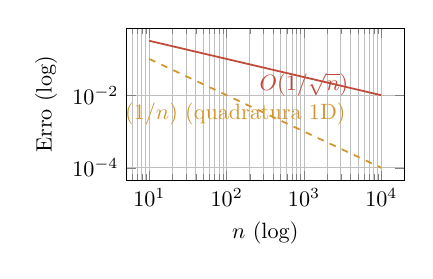
\begin{tikzpicture}[scale=0.8]
\begin{axis}[
    xlabel={$n$ (log)},
    ylabel={Erro (log)},
    width=6cm, height=4cm,
    xmode=log, ymode=log,
    grid=both,
]
\addplot[wp-primary, thick, domain=10:10000, samples=100] {1/sqrt(x)};
\node[wp-primary] at (axis cs:1000, 0.02) {$O(1/\sqrt{n})$};
\addplot[wp-accent, thick, dashed, domain=10:10000, samples=100] {1/x};
\node[wp-accent] at (axis cs:100, 0.003) {$O(1/n)$ (quadratura 1D)};
\end{axis}
\end{tikzpicture}
\caption{Taxa de convergência do erro de Monte Carlo vs. quadratura numérica em 1D.
Em dimensão alta, a quadratura torna-se inviável; MC não.}
\end{marginfigure}

\paragraph{Amostragem por Importância}

E se não pudermos amostrar diretamente de $p(x)$? Ou se $p(x)$ for muito concentrada
em regiões onde $f(x)$ é pequeno? A \textbf{amostragem por importância} resolve ambos:

\begin{defn}[ Amostragem por Importância]
    Seja $q(x)$ uma distribuição (a \textbf{proposta}) que podemos amostrar.
    Então:
    \[
    \E_{p}[f(X)] = \int f(x) p(x) dx = \int f(x) \frac{p(x)}{q(x)} q(x) dx = \E_{q}\left[f(X) \frac{p(X)}{q(X)}\right]
    \]
    O estimador é:
    \[
    \hat{\mu}_{\text{IS}} = \frac{1}{n} \sum_{i=1}^n f(X_i) \underbrace{\frac{p(X_i)}{q(X_i)}}_{w(X_i)}
    \]
    onde $X_i \sim q$ e $w(X_i)$ são os \textbf{pesos de importância}.
\end{defn}

A escolha da proposta $q$ é crítica. Idealmente, $q$ deve ser proporcional a $|f(x)| p(x)$
(amostragem nas regiões que mais importam). Na prática, encontrar uma boa $q$ é uma arte.

\paragraph{Aplicações em ML}

\begin{enumerate}
    \item \textbf{Dropout como MC}: Gal \& Ghahramani (2016) mostraram que dropout durante
    o treinamento, quando mantido ativo na inferência, produz amostras de uma distribuição
    aproximada sobre os pesos --- uma forma de Monte Carlo.
    \item \textbf{Gradientes Estocásticos}: SGD amostra mini-lotes para estimar o gradiente
    completo --- um estimador de Monte Carlo do gradiente esperado.
    \item \textbf{Avaliação de Modelos}: Estimamos o erro de generalização por Monte Carlo
    sobre a distribuição dos dados (conjunto de teste é uma amostra).
    \item \textbf{Bootstrapping}: Amostragem com reposição dos dados para estimar a
    variabilidade de estimadores.
\end{enumerate}

\section{Markov Chain Monte Carlo (MCMC)}
\label{sec:mcmc}

\paragraph{A Limitação do Monte Carlo Clássico}

O Monte Carlo clássico exige amostras independentes de $p(x)$. Mas para muitas
distribuições de interesse em ML (particularmente posteriores complexas), não sabemos
como amostrar diretamente, e a amostragem por importância falha em altas dimensões
(os pesos tornam-se degenerados --- quase todas as amostras têm peso zero).

O MCMC resolve este problema: em vez de amostrar independentemente, construímos uma
cadeia de Markov cuja distribuição estacionária é $p(x)$. Amostramos da cadeia após
ela ter ``queimado'' (burn-in) e atingido o equilíbrio.

\begin{exmp}[Analogia do Cachorro Perdido]
    Imagine um cachorro perdido em uma floresta à noite. Você quer amostrar locais
    onde o cachorro pode estar (distribuição $p$). Você não sabe $p$ analiticamente,
    mas sabe a probabilidade relativa de dois locais adjacentes (razão $p(x')/p(x)$).

    O cachorro anda aleatoriamente: de sua posição atual $x$, ele propõe um passo
    $x'$. Se $p(x') > p(x)$, ele aceita o passo (vai para um lugar melhor).
    Se $p(x') < p(x)$, ele aceita com probabilidade $p(x')/p(x)$ (às vezes fica,
    às vezes volta). Com o tempo, o cachorro passa mais tempo em regiões de alta
    probabilidade --- sua trajetória é uma amostra de $p$.
\end{exmp}

\subsection{O Algoritmo Metropolis--Hastings}

\begin{algorithm}[h]
\caption{Metropolis--Hastings}
\begin{itemize}
    \item Inicialize $x^{(0)}$.
    \item Para $t = 1, 2, \dots, T$:
    \begin{enumerate}
        \item Proponha $x^* \sim q(x^* \mid x^{(t-1)})$.
        \item Calcule a razão de aceitação:
        \[
        \alpha = \min\left(1, \frac{p(x^*)}{p(x^{(t-1)})} \cdot \frac{q(x^{(t-1)} \mid x^*)}{q(x^* \mid x^{(t-1)})} \right)
        \]
        \item Aceite $x^{(t)} = x^*$ com probabilidade $\alpha$; caso contrário,
        $x^{(t)} = x^{(t-1)}$.
    \end{enumerate}
\end{itemize}
\end{algorithm}

A beleza do algoritmo é que ele só precisa da razão $p(x^*)/p(x^{(t-1)})$ --- as constantes
normalizadoras se cancelam. Isto é crucial para inferência bayesiana, onde
$p(x) = \tilde{p}(x)/Z$ com $Z$ intratável.

\begin{proof}[Por que Metropolis--Hastings funciona]
    O algoritmo define uma cadeia de Markov com núcleo de transição:
    \[
    K(x, x') = q(x' \mid x) \alpha(x, x') + \delta_x(x') \left(1 - \int q(y \mid x) \alpha(x, y) dy\right)
    \]
    O balanço detalhado é satisfeito:
    \[
    p(x) K(x, x') = p(x') K(x', x)
    \]
    verificável por construção de $\alpha$. Portanto, $p$ é a distribuição estacionária
    da cadeia. Se a cadeia é irredutível e aperiódica, a distribuição das amostras
    converge para $p$.
\end{proof}

\subsection{Amostrador de Gibbs}

Um caso especial importante do Metropolis--Hastings é o \textbf{amostrador de Gibbs},
que amostra cada coordenada condicional às demais:

\begin{algorithm}[h]
\caption{Amostrador de Gibbs}
\begin{itemize}
    \item Inicialize $x^{(0)} = (x_1^{(0)}, \dots, x_d^{(0)})$.
    \item Para $t = 1, 2, \dots, T$:
    \begin{enumerate}
        \item Para $j = 1, \dots, d$:
        \[
        x_j^{(t)} \sim p(x_j \mid x_1^{(t)}, \dots, x_{j-1}^{(t)}, x_{j+1}^{(t-1)}, \dots, x_d^{(t-1)})
        \]
    \end{enumerate}
\end{itemize}
\end{algorithm}

O amostrador de Gibbs sempre aceita a proposta (taxa de aceitação = 1), mas exige que
saibamos amostrar das condicionais completas. É amplamente usado em modelos gráficos
e tópicos (LDA).

\subsection{Desafios Práticos do MCMC}

\begin{enumerate}
    \item \textbf{Burn-in}: As primeiras amostras dependem da inicialização e não
    representam a distribuição-alvo. Devem ser descartadas.
    \item \textbf{Correlação}: Amostras consecutivas são correlacionadas. O \textbf{tamanho
    efetivo da amostra} (ESS) é menor que o número de amostras:
    \[
    n_{\text{eff}} = \frac{n}{1 + 2\sum_{k=1}^\infty \rho_k}
    \]
    onde $\rho_k$ é a autocorrelação no lag $k$.
    \item \textbf{Thinning}: Para reduzir correlação, guardamos apenas uma a cada $k$
    amostras (ex: a cada 10 passos).
    \item \textbf{Mixing}: A cadeia pode ficar presa em modos locais, especialmente
    em distribuições multimodais.
    \item \textbf{Diagnóstico}: Usamos $\hat{R}$ (Gelman--Rubin) para verificar
    convergência: execute múltiplas cadeias e compare variância dentro vs. entre cadeias.
    $\hat{R} \approx 1$ indica convergência.
\end{enumerate}

\subsection{MCMC em Aprendizado de Máquina}

\begin{enumerate}
    \item \textbf{Inferência Bayesiana em Redes Neurais}: Amostragem da posterior dos
    pesos para quantificar incerteza (BNN com MCMC).
    \item \textbf{Modelos de Tópicos (LDA)}: Gibbs sampling é o algoritmo padrão para
    treinar Latent Dirichlet Allocation.
    \item \textbf{Modelos Gaussianos Latentes}: MCMC para inferência em GP e modelos
    relacionados.
    \item \textbf{Deep Learning Probabilístico}: Métodos MCMC modernos (HMC, NUTS) são
    usados em frameworks probabilísticos como Stan e PyMC.
\end{enumerate}

%%%%%%%%%%%%%%%%%%%%%%%%%%%%%%%%%%%%%%%%%%%%%%%%%%%%%%%%%%%%%%%%%%%%%%%%%%%%%%%%
% PART IV: TEORIA DA INFORMAÇÃO
%%%%%%%%%%%%%%%%%%%%%%%%%%%%%%%%%%%%%%%%%%%%%%%%%%%%%%%%%%%%%%%%%%%%%%%%%%%%%%%%

\part{Teoria da Informação}

\section{Entropia e Incerteza}

\paragraph{Claude Shannon e o Problema da Comunicação}

Em 1948, Claude Shannon, engenheiro do Bell Labs, publicou \textit{A Mathematical Theory
of Communication}, fundando a teoria da informação. Seu problema era prático: como
transmitir informação de forma eficiente através de um canal ruidoso?

Shannon percebeu que a informação era uma quantidade mensurável --- e que a incerteza
era sua moeda.

\paragraph{Motivação: Quantos bits?}

Imagine que você quer saber o resultado de um experimento com $m$ resultados igualmente
prováveis. Quantas perguntas binárias (sim/não) você precisa fazer, em média?

\begin{exmp}[O Jogo dos 20 Bichos]
    Pense em um animal. Quantas perguntas fechadas são necessárias para adivinhá-lo?
    Se o animal é escolhido uniformemente de um conjunto de $2^{20} \approx 1$ milhão
    de possibilidades, você precisa de 20 perguntas (cada pergunta divide o espaço pela
    metade). Isto é $\log_2(2^{20}) = 20$ bits.

    Shannon formalizou esta intuição: a quantidade de informação associada a um evento
    com probabilidade $p$ é $-\log_2(p)$. Um evento certo ($p=1$) tem 0 bits de
    informação (nenhuma surpresa). Um evento improvável ($p \approx 0$) tem muitos bits
    (grande surpresa).
\end{exmp}

\begin{defn}[Entropia]
    A \textbf{entropia} de uma variável aleatória discreta $X$ com distribuição $p$ é:
    \[
    H(X) = -\sum_{x} p(x) \log p(x) = \E[-\log p(X)]
    \]
    Usamos $\log$ base 2 para bits ou base $e$ para nats. Por convenção, $0\log 0 = 0$.
\end{defn}

A entropia mede a incerteza média sobre o valor de $X$. É o número mínimo de bits
necessários, em média, para codificar $X$ de forma ótima.

\begin{exmp}
    \begin{itemize}
        \item Moeda justa: $H = -(0.5\log 0.5 + 0.5\log 0.5) = 1$ bit.
        \item Moeda viciada ($p=0.9$): $H = -(0.9\log 0.9 + 0.1\log 0.1) \approx 0.47$ bits.
        \item Moeda determinística ($p=1$): $H = -(1\log 1 + 0\log 0) = 0$ bits.
    \end{itemize}
\end{exmp}

\subsection{Entropia Cruzada e Divergência KL}

\begin{defn}[Entropia Cruzada]
    A \textbf{entropia cruzada} entre duas distribuições $p$ e $q$ sobre o mesmo espaço é:
    \[
    H(p, q) = -\sum_{x} p(x) \log q(x) = H(p) + \KL(p \parallel q)
    \]
\end{defn}

A entropia cruzada mede o número médio de bits necessários para codificar amostras de
$p$ usando um código ótimo para $q$. Quanto maior a diferença entre $p$ e $q$, maior
a entropia cruzada.

\begin{defn}[Divergência de Kullback--Leibler (KL)]
    A divergência KL entre $p$ e $q$ é:
    \[
    \KL(p \parallel q) = \sum_{x} p(x) \log \frac{p(x)}{q(x)} = \E_{p}\left[\log \frac{p(X)}{q(X)}\right]
    \]
\end{defn}

\begin{prop}[Propriedades da Divergência KL]
    \begin{enumerate}
        \item $\KL(p \parallel q) \ge 0$, com igualdade sse $p = q$ (desigualdade de Gibbs).
        \item $\KL(p \parallel q) \neq \KL(q \parallel p)$ (não é simétrica).
        \item $\KL(p \parallel q) = \infty$ se existe $x$ com $p(x) > 0$ e $q(x) = 0$.
    \end{enumerate}
\end{prop}

A divergência KL é uma ``distância'' entre distribuições (embora não seja simétrica nem
satisfaça a desigualdade triangular). É a medida fundamental de dissimilaridade em teoria
da informação.

\paragraph{Divergência KL e Máxima Verossimilhança}

Suponha que temos dados $\{x_i\}_{i=1}^n \sim p_{\text{data}}$ e queremos ajustar um
modelo $p_\theta$. O estimador de máxima verossimilhança (MLE) minimiza a entropia
cruzada entre $p_{\text{data}}$ e $p_\theta$:
\[
\hat{\theta}_{\text{MLE}} = \argmin_\theta -\frac{1}{n}\sum_{i=1}^n \log p_\theta(x_i)
\]
Para $n$ grande, isto é equivalente a minimizar $\KL(p_{\text{data}} \parallel p_\theta)$:
\[
-\frac{1}{n}\sum_{i=1}^n \log p_\theta(x_i) \approx \E_{p_{\text{data}}}[-\log p_\theta(X)] = H(p_{\text{data}}, p_\theta) = H(p_{\text{data}}) + \KL(p_{\text{data}} \parallel p_\theta)
\]
Como $H(p_{\text{data}})$ é constante, minimizar a perda é o mesmo que minimizar KL.

\paragraph{Aplicações em ML}
\begin{enumerate}
    \item \textbf{Classificação}: A perda de entropia cruzada é a função de perda padrão
    para classificação (cross-entropy loss).
    \item \textbf{VAEs}: O termo de regularização de um VAE é $\KL(q(z\mid x) \parallel p(z))$,
    onde $q$ é o encoder e $p$ é a priori latente.
    \item \textbf{Knowledge Distillation}: Destilar conhecimento de um modelo grande
    para um pequeno minimiza KL entre suas distribuições de saída.
    \item \textbf{Policy Gradient}: Algoritmos de RL como TRPO e PPO usam KL para
    limitar mudanças na política.
\end{enumerate}

\subsection{Informação Mútua}

\begin{defn}[Informação Mútua]
    A \textbf{informação mútua} entre duas variáveis aleatórias $X$ e $Y$ é:
    \[
    I(X; Y) = \KL(p(x,y) \parallel p(x)p(y)) = \sum_{x,y} p(x,y) \log \frac{p(x,y)}{p(x)p(y)}
    \]
\end{defn}

A informação mútua mede quanta informação $X$ contém sobre $Y$ (e vice-versa).
É zero sse $X$ e $Y$ são independentes.

\begin{prop}
    \begin{align*}
        I(X; Y) &= H(X) - H(X \mid Y) \\
        I(X; Y) &= H(Y) - H(Y \mid X) \\
        I(X; Y) &= H(X) + H(Y) - H(X, Y) \\
        I(X; Y) &\ge 0
    \end{align*}
\end{prop}

Em aprendizado de máquina:
\begin{enumerate}
    \item \textbf{Seleção de features}: Features com alta informação mútua com o target
    são mais relevantes.
    \item \textbf{InfoGAN}: Adiciona um termo de informação mútua entre o código latente
    e a saída do gerador para aprendizado não-supervisionado de representações
    interpretáveis.
    \item \textbf{Information Bottleneck}: Busca-se um trade-off entre compressão do input
    e preservação de informação sobre o target.
\end{enumerate}

\part{Estruturas Probabilísticas para Modelagem}

Chegamos a um ponto de inflexão em nossa jornada. Nos capítulos anteriores, construímos os fundamentos --- probabilidade, cadeias de Markov, Monte Carlo, teoria da informação --- e vimos como estimadores emergem naturalmente do princípio da verossimilhança. Agora, a pergunta muda de figura: como \textit{modelamos} estruturas complexas? Como lidamos com dados que não são meros números i.i.d., mas sim textos, imagens, sequências genéticas, séries temporais?

A resposta passa por cinco grandes ideias, que exploraremos em sequência. Primeiro, as \textbf{famílias exponenciais}, a classe mais elegante e útil de distribuições. Depois, as \textbf{priors conjugadas}, que tornam a inferência Bayesiana analítica e interpretável. Os \textbf{modelos gráficos probabilísticos} nos dão uma linguagem visual e algébrica para representar dependências complexas. O \textbf{algoritmo EM} é a ferramenta computacional que torna possível estimar parâmetros na presença de variáveis latentes. E, finalmente, os \textbf{processos Gaussianos} nos mostram como levar a Gaussianidade ao infinito --- distribuições sobre funções.

Cada uma dessas ideias é, por si só, um campo maduro. Mas, juntas, elas formam o alicerce sobre o qual o aprendizado de máquina moderno foi construído.

%===============================================================================
\section{Famílias Exponenciais}
%===============================================================================

\paragraph{O problema da unificação.}

Ao longo deste texto, encontramos dezenas de distribuições: Bernoulli, Binomial, Poisson, Gaussiana, Beta, Gamma, Dirichlet. Cada uma tem sua própria parametrização, seu próprio conjunto de identidades, suas próprias propriedades. Há uma sensação incômoda de repetição --- muitas dessas distribuições compartilham estrutura, mas essa estrutura raramente é explícita.

As \textbf{famílias exponenciais} surgem exatamente para resolver esse problema. Elas unificam uma vasta classe de distribuições sob uma única forma matemática, revelando a estrutura comum que subjaz a Bernoulli e Gaussiana, a Poisson e Dirichlet.

\begin{defn}[Família Exponencial]
    Uma família de distribuições $\{p(\cdot \mid \theta) : \theta \in \Theta\}$ pertence à \textbf{família exponencial} se pode ser escrita na forma:
    \[
    p(x \mid \theta) = h(x) \exp\big(\eta(\theta)^T T(x) - A(\theta)\big)
    \]
    onde:
    \begin{itemize}
        \item $h(x)$ é a \textbf{medida base} (muitas vezes um termo de normalização que depende apenas de $x$);
        \item $\eta(\theta)$ é o \textbf{parâmetro natural};
        \item $T(x)$ é a \textbf{estatística suficiente};
        \item $A(\theta)$ é a \textbf{função de log-partição} (também chamada de cumulante).
    \end{itemize}
\end{defn}

A função $A(\theta)$ merece atenção especial. Ela é o logaritmo da constante de normalização:
\[
A(\theta) = \log \int h(x) \exp\big(\eta(\theta)^T T(x)\big) \, dx
\]
e, como veremos, suas derivadas codificam os momentos da distribuição.

\paragraph{Forma canônica.}

Quando parametrizamos a distribuição pelo parâmetro natural $\eta$ diretamente --- isto é, tratamos $\eta$ como o parâmetro --- dizemos que a família está em \textbf{forma canônica}:
\[
p(x \mid \eta) = h(x) \exp\big(\eta^T T(x) - A(\eta)\big)
\]

A forma canônica é particularmente útil porque o espaço de parâmetros $\eta$ é convexo, e $A(\eta)$ é uma função convexa. Isso transforma problemas de inferência em problemas de otimização convexa, com todas as garantias que isso implica.

\begin{exmp}[Bernoulli na forma canônica]
    A Bernoulli com parâmetro $\mu \in [0,1]$ tem densidade:
    \[
    p(x \mid \mu) = \mu^x (1-\mu)^{1-x} = \exp\big(x \log \mu + (1-x) \log(1-\mu)\big)
    \]
    Reorganizando:
    \[
    p(x \mid \mu) = \exp\!\left(x \log\frac{\mu}{1-\mu} + \log(1-\mu)\right)
    \]
    Identificamos:
    \[
    \eta = \log\frac{\mu}{1-\mu}, \quad T(x) = x, \quad A(\eta) = \log(1 + e^\eta), \quad h(x) = 1
    \]
    A inversa $\mu = \sigma(\eta) = 1/(1+e^{-\eta})$ é a função logística.
\end{exmp}

\paragraph{Exemplos clássicos.}

Vejamos como diversas distribuições familiares se encaixam nesse molde unificado:

\begin{itemize}
    \item \textbf{Bernoulli}: $T(x) = x$, $\eta = \log(\mu/(1-\mu))$, $A(\eta) = \log(1+e^\eta)$.
    
    \item \textbf{Poisson}: $p(x \mid \lambda) = \lambda^x e^{-\lambda}/x!$. Temos $\eta = \log\lambda$, $T(x)=x$, $A(\eta) = e^\eta$, $h(x) = 1/x!$.
    
    \item \textbf{Gaussiana} (variância conhecida $\sigma^2$):
    \[
    p(x \mid \mu) = \frac{1}{\sqrt{2\pi\sigma^2}} \exp\!\left(-\frac{(x-\mu)^2}{2\sigma^2}\right)
    \]
    que se reescreve como:
    \[
    p(x \mid \mu) = \exp\!\left(\frac{\mu}{\sigma^2} x - \frac{\mu^2}{2\sigma^2} - \frac{x^2}{2\sigma^2} - \frac{1}{2}\log(2\pi\sigma^2)\right)
    \]
    Neste caso, $\eta = \mu/\sigma^2$, $T(x) = x$, $A(\eta) = \frac{\sigma^2\eta^2}{2}$.
    
    \item \textbf{Beta}:
    \[
    p(x \mid \alpha, \beta) = \frac{\Gamma(\alpha+\beta)}{\Gamma(\alpha)\Gamma(\beta)} x^{\alpha-1} (1-x)^{\beta-1}
    \]
    Temos $\eta = [\alpha-1, \beta-1]^T$, $T(x) = [\log x, \log(1-x)]^T$.
    
    \item \textbf{Gamma}:
    \[
    p(x \mid \alpha, \beta) = \frac{\beta^\alpha}{\Gamma(\alpha)} x^{\alpha-1} e^{-\beta x}
    \]
    Para forma com $\alpha$ conhecido: $\eta = -\beta$, $T(x) = x$, $A(\eta) = -\alpha\log(-\eta)$.
    
    \item \textbf{Dirichlet}: generalização da Beta para $K$ categorias:
    \[
    p(\mathbf{x} \mid \boldsymbol{\alpha}) = \frac{\Gamma(\sum \alpha_k)}{\prod \Gamma(\alpha_k)} \prod_{k=1}^K x_k^{\alpha_k-1}
    \]
    com $T(x) = [\log x_1, \dots, \log x_K]^T$, $\eta_k = \alpha_k - 1$.
    
    \item \textbf{Categórica} (Multinomial com $n=1$):
    \[
    p(x \mid \boldsymbol{\pi}) = \prod_{k=1}^K \pi_k^{\mathbbm{1}[x=k]}
    \]
    com $T(x) = [\mathbbm{1}[x=1], \dots, \mathbbm{1}[x=K]]^T$, $\eta_k = \log(\pi_k/\pi_K)$.
\end{itemize}

\paragraph{Estatísticas suficientes e o teorema de Fisher-Neyman.}

A beleza da forma da família exponencial está no papel de $T(x)$. Toda a informação que os dados $x$ contêm sobre o parâmetro $\theta$ é resumida por $T(x)$. Não importa quão grande seja a amostra --- se temos $n$ pontos $x_1,\dots,x_n$, a estatística $\sum_{i=1}^n T(x_i)$ é \textbf{suficiente}: a distribuição condicional dos dados dado esse resumo não depende de $\theta$.

O \textbf{teorema de Fisher-Neyman} formaliza essa intuição: uma estatística $T(X)$ é suficiente para $\theta$ se e somente se a densidade fatora como:
\[
p(x \mid \theta) = g(T(x), \theta) \cdot h(x)
\]
que é exatamente a estrutura que vemos na família exponencial. A função $h(x)$ absorve os termos que não dependem de $\theta$; $g(T(x), \theta)$ contém toda a dependência.

\paragraph{Momentos via derivadas de $A(\theta)$.}

Aqui está talvez a propriedade mais útil da família exponencial: a função de log-partição $A(\theta)$ é um \textbf{gerador de cumulantes}. Suas derivadas nos dão os momentos da distribuição.

\begin{thm}[Momentos da família exponencial]
    Para uma família exponencial na forma canônica $p(x \mid \eta) = h(x) \exp(\eta^T T(x) - A(\eta))$:
    \begin{align*}
        \E[T(x)] &= \nabla A(\eta) \\
        \Var[T(x)] &= \nabla^2 A(\eta)
    \end{align*}
    onde $\nabla A$ é o gradiente e $\nabla^2 A$ é a matriz Hessiana de $A$.
\end{thm}

\begin{proof}
    Da definição $A(\eta) = \log \int h(x) e^{\eta^T T(x)} dx$, derivamos:
    \[
    \nabla A(\eta) = \frac{\int h(x) T(x) e^{\eta^T T(x)} dx}{\int h(x) e^{\eta^T T(x)} dx} = \E[T(x)]
    \]
    A segunda derivada segue de forma análoga:
    \[
    \nabla^2 A(\eta) = \E[T(x)T(x)^T] - \E[T(x)]\E[T(x)]^T = \Var[T(x)]
    \]
\end{proof}

Isso é notável: não precisamos calcular nenhuma integral explicitamente. Derivamos $A$ e obtemos momentos.

Para a Bernoulli, por exemplo, $A(\eta) = \log(1+e^\eta)$:
\[
\frac{dA}{d\eta} = \frac{e^\eta}{1+e^\eta} = \sigma(\eta) = \mu, \quad \frac{d^2A}{d\eta^2} = \sigma(\eta)(1-\sigma(\eta)) = \mu(1-\mu)
\]

\begin{remark}
    A relação entre derivadas de $A$ e momentos se estende para ordens superiores. A terceira derivada dá o terceiro cumulante (assimetria), a quarta dá o quarto (curtose), e assim por diante.
\end{remark}

\paragraph{Relação com GLMs.}

As famílias exponenciais são a espinha dorsal dos \textbf{Modelos Lineares Generalizados} (GLMs). Em um GLM, modelamos a média $\mu = \E[Y \mid X]$ como:
\[
g(\mu) = \beta^T X
\]
onde $g$ é a \textbf{função de ligação}. Quando escolhemos $g$ como a função que mapeia a média ao parâmetro natural --- isto é, $g(\mu) = \eta$ --- obtemos a \textbf{ligação canônica}.

Para cada família exponencial, a ligação canônica é:
\begin{itemize}
    \item Gaussiana: $g(\mu) = \mu$ (identidade)
    \item Bernoulli: $g(\mu) = \log(\mu/(1-\mu))$ (logit)
    \item Poisson: $g(\mu) = \log \mu$ (log)
    \item Gamma: $g(\mu) = 1/\mu$ (inversa)
\end{itemize}

A ligação canônica simplifica a inferência porque a estatística suficiente se torna linear nos parâmetros, e o gradiente da log-verossimilhança tem forma particularmente simples.

\begin{remark}
    Por que famílias exponenciais são fundamentais para análise conjugada? Como veremos na próxima seção, quando a likelihood pertence a uma família exponencial, existe uma prior --- também de família exponencial --- que produz uma posterior na mesma família. A função de log-partição $A(\theta)$ codifica os momentos, e a atualização Bayesiana se reduz a uma soma algébrica de estatísticas suficientes.
\end{remark}

%===============================================================================
\section{Priors Conjugadas e Inferência Analítica}
%===============================================================================

\paragraph{O sonho de Bayes.}

Em 1763, o reverendo Thomas Bayes --- ou talvez seu amigo Richard Price, que publicou o ensaio póstumo --- propôs um problema simples: dada uma sequência de tentativas Bernoulli com probabilidade de sucesso desconhecida $\theta$, como atualizamos nossa crença sobre $\theta$ ao observar dados?

A resposta de Bayes foi surpreendentemente elegante: se nossa crença inicial sobre $\theta$ segue uma distribuição $\text{Beta}(\alpha, \beta)$, então após observar $N$ sucessos em $n$ tentativas, nossa crença atualizada é $\text{Beta}(\alpha + N, \beta + n - N)$. A posterior tem a \textbf{mesma forma} que a prior. Isso é uma \textbf{prior conjugada}.

\begin{defn}[Prior Conjugada]
    Uma família de distribuições $\mathcal{F}$ é \textbf{conjugada} a uma likelihood $p(x \mid \theta)$ se, para qualquer prior $p(\theta) \in \mathcal{F}$, a posterior $p(\theta \mid x) \propto p(x \mid \theta) p(\theta)$ também pertence a $\mathcal{F}$.
\end{defn}

Quando isso acontece, a inferência Bayesiana se reduz a uma simples atualização dos parâmetros da prior. Não precisamos de integração numérica, MCMC, ou aproximações variacionais --- a matemática é exata e fechada.

\paragraph{Tabela de relações de conjugação.}

A natureza generosa do universo matemático nos presenteia com conjugação para praticamente todas as combinações clássicas de likelihood e prior:

\begin{itemize}
    \item \textbf{Beta-Bernoulli / Beta-Binomial}: Se $X_i \sim \Bern(\theta)$ e $\theta \sim \Beta(\alpha, \beta)$, então:
    \[
    \theta \mid X_{1:n} \sim \Beta\!\left(\alpha + \sum x_i, \beta + n - \sum x_i\right)
    \]
    
    \item \textbf{Dirichlet-Categórica / Dirichlet-Multinomial}: Se $\mathbf{x}_i \sim \Cat(\boldsymbol{\theta})$ e $\boldsymbol{\theta} \sim \Dir(\boldsymbol{\alpha})$, então:
    \[
    \boldsymbol{\theta} \mid \mathbf{x}_{1:n} \sim \Dir\!\left(\boldsymbol{\alpha} + \sum_{i=1}^n \mathbbm{1}_{\mathbf{x}_i}\right)
    \]
    
    \item \textbf{Gamma-Poisson}: Se $X_i \sim \Pois(\lambda)$ e $\lambda \sim \Gam(\alpha, \beta)$, então:
    \[
    \lambda \mid X_{1:n} \sim \Gam\!\left(\alpha + \sum x_i, \beta + n\right)
    \]
    
    \item \textbf{Gaussiana-Gaussiana} (variância conhecida $\sigma^2$): Se $X_i \sim \N(\mu, \sigma^2)$ e $\mu \sim \N(\mu_0, \sigma_0^2)$, então:
    \[
    \mu \mid X_{1:n} \sim \N\!\left(\frac{\mu_0/\sigma_0^2 + n\bar{x}/\sigma^2}{1/\sigma_0^2 + n/\sigma^2},\; \frac{1}{1/\sigma_0^2 + n/\sigma^2}\right)
    \]
    
    \item \textbf{Gaussiana-Gamma Inversa} (variância desconhecida): Se $X_i \sim \N(\mu, \sigma^2)$ e $\sigma^2 \sim \IG(\alpha, \beta)$, então:
    \[
    \sigma^2 \mid X_{1:n} \sim \IG\!\left(\alpha + \frac{n}{2},\; \beta + \frac{1}{2}\sum_{i=1}^n (x_i - \mu)^2\right)
    \]
    
    \item \textbf{Gamma-Exponencial}: Se $X_i \sim \text{Exp}(\lambda)$ e $\lambda \sim \Gam(\alpha, \beta)$, então:
    \[
    \lambda \mid X_{1:n} \sim \Gam\!\left(\alpha + n,\; \beta + \sum x_i\right)
    \]
    
    \item \textbf{Wishart-Inverse Wishart} (matrizes de covariância): Para dados Gaussianos multivariados $\mathbf{x}_i \sim \N(\boldsymbol{\mu}, \boldsymbol{\Sigma})$, se $\boldsymbol{\Sigma} \sim \InvWish(\Psi, \nu)$, então:
    \[
    \boldsymbol{\Sigma} \mid \mathbf{X} \sim \InvWish\!\left(\Psi + \sum_{i=1}^n (\mathbf{x}_i - \boldsymbol{\mu})(\mathbf{x}_i - \boldsymbol{\mu})^T,\; \nu + n\right)
    \]
\end{itemize}

\paragraph{Derivação detalhada: Beta-Bernoulli.}

Vejamos com calma como a conjugação funciona para o caso mais simples, que é também o mais instrutivo.

\textbf{Modelo:} Seja $X_1, \dots, X_n \in \{0,1\}$ i.i.d. com $P(X_i = 1) = \theta$. A likelihood é:
\[
p(\mathbf{x} \mid \theta) = \prod_{i=1}^n \theta^{x_i} (1-\theta)^{1-x_i} = \theta^{\sum x_i} (1-\theta)^{n - \sum x_i}
\]

\textbf{Prior:} Escolhemos $\theta \sim \Beta(\alpha, \beta)$:
\[
p(\theta) = \frac{\Gamma(\alpha+\beta)}{\Gamma(\alpha)\Gamma(\beta)} \theta^{\alpha-1} (1-\theta)^{\beta-1}, \quad \theta \in [0,1]
\]

\textbf{Posterior:} Pelo teorema de Bayes:
\[
p(\theta \mid \mathbf{x}) \propto p(\mathbf{x} \mid \theta) \cdot p(\theta)
\]
\[
p(\theta \mid \mathbf{x}) \propto \theta^{\sum x_i} (1-\theta)^{n - \sum x_i} \cdot \theta^{\alpha-1} (1-\theta)^{\beta-1}
\]
\[
p(\theta \mid \mathbf{x}) \propto \theta^{\alpha + \sum x_i - 1} (1-\theta)^{\beta + n - \sum x_i - 1}
\]

Esta é exatamente a forma de uma distribuição Beta:
\[
\theta \mid \mathbf{x} \sim \Beta\!\left(\alpha + \sum x_i,\; \beta + n - \sum x_i\right)
\]

A interpretação é bela: os parâmetros $\alpha$ e $\beta$ da prior funcionam como ``pseudo-contagens'' --- $\alpha$ sucessos e $\beta$ fracassos observados antes dos dados reais. Ao observar $N = \sum x_i$ sucessos em $n$ tentativas, simplesmente somamos: $\alpha + N$ e $\beta + (n-N)$.

\begin{remark}
    O parâmetro $\alpha + \beta$ da prior controla a \textbf{força} da crença inicial. Quanto maior $\alpha + \beta$, mais dados são necessários para mover a posterior significativamente. Quando $\alpha = \beta = 1$, a prior é uniforme --- máxima incerteza inicial.
\end{remark}

\paragraph{Distribuição preditiva posterior.}

Uma das grandes vantagens da inferência Bayesiana analítica é a capacidade de fazer previsões sem aproximação. A \textbf{distribuição preditiva posterior} $p(\tilde{x} \mid \mathbf{x})$ nos diz quão provável é um novo dado $\tilde{x}$ dado o que já observamos:

\[
p(\tilde{x} \mid \mathbf{x}) = \int p(\tilde{x} \mid \theta) p(\theta \mid \mathbf{x}) \, d\theta
\]

Para combinações conjugadas, essa integral tem forma fechada:

\begin{itemize}
    \item \textbf{Beta-Binomial} (modelo Beta-Bernoulli, preditiva para $m$ novas tentativas):
    \[
    p(\tilde{N} \mid \mathbf{x}) = \binom{m}{\tilde{N}} \frac{B(\alpha + N + \tilde{N},\; \beta + (n-N) + (m-\tilde{N}))}{B(\alpha + N,\; \beta + n - N)}
    \]
    que é uma \textbf{Beta-Binomial} --- uma distribuição que parece Binomial mas com caudas mais pesadas, refletindo a incerteza sobre $\theta$.
    
    \item \textbf{Gamma-Poisson} (preditiva para um novo ponto):
    \[
    p(\tilde{x} \mid \mathbf{x}) = \frac{\Gamma(\tilde{x} + \alpha + n)}{\tilde{x}! \,\Gamma(\alpha + n)} \left(\frac{\beta + n}{\beta + n + 1}\right)^{\alpha + n} \left(\frac{1}{\beta + n + 1}\right)^{\tilde{x}}
    \]
    que é uma \textbf{Binomial Negativa} --- novamente, caudas mais pesadas que a Poisson.
    
    \item \textbf{Gaussiana-Gaussiana} (preditiva para um novo ponto, variância conhecida):
    \[
    \tilde{x} \mid \mathbf{x} \sim \N\!\left(\mu_n,\; \sigma^2 + \sigma_n^2\right)
    \]
    onde $\mu_n$ e $\sigma_n^2$ são a média e variância posteriores. A incerteza preditiva combina a variância dos dados ($\sigma^2$) com a incerteza sobre $\mu$ ($\sigma_n^2$). Esta é uma distribuição \textbf{t-Student} quando a variância é desconhecida e integrada analiticamente.
\end{itemize}

\begin{remark}
    A preditiva posterior revela um princípio crucial: a incerteza sobre parâmetros ``se propaga'' para as previsões. Modelos Bayesianos produzem naturalmente distribuições preditivas mais dispersas que modelos plug-in (que usam apenas $\hat{\theta}_{\text{MLE}}$), refletindo corretamente nossa incerteza.
\end{remark}

\paragraph{Por que a conjugação importa.}

A conjugação não é apenas uma elegância matemática. Ela resolve problemas práticos fundamentais:

\begin{enumerate}
    \item \textbf{Inferência em tempo real}: Em sistemas de recomendação, monitoramento de sensores, ou classificação online, a atualização Bayesiana se reduz a manter contagens e somas --- operações $O(1)$.
    \item \textbf{Interpretabilidade}: Os parâmetros da prior têm significado intuitivo (pseudo-contagens, somas de quadrados), facilitando a comunicação com especialistas de domínio.
    \item \textbf{Base para métodos mais complexos}: Modelos hierárquicos, processos de Dirichlet, e inferência variacional frequentemente exploram a conjugação local para obter atualizações fechadas.
\end{enumerate}

\begin{exmp}[Aprendizado online com Beta-Bernoulli]
    Imagine um sistema de recomendação que modela a probabilidade de um usuário gostar de um filme. Começamos com prior $\Beta(1,1)$ (incerteza total). A cada interação:
    \begin{itemize}
        \item Se o usuário gosta: atualizamos $\alpha \leftarrow \alpha + 1$.
        \item Se não gosta: atualizamos $\beta \leftarrow \beta + 1$.
    \end{itemize}
    A média posterior $\alpha/(\alpha+\beta)$ converge para a verdadeira preferência do usuário, e a variância posterior nos diz quão certos estamos. Após poucas interações, a incerteza cai drasticamente.
\end{exmp}

\paragraph{Limitações.}

A conjugação, contudo, não é uma bala de prata. Ela tem limitações importantes:

\begin{itemize}
    \item \textbf{Disponibilidade}: Nem toda distribuição tem uma conjugada conhecida. Para muitas likelihoods modernas (redes neurais, modelos com variáveis latentes complexas), a conjugação não existe.
    \item \textbf{Expressividade limitada}: Priors conjugadas são muitas vezes restritivas. Uma Beta-Bernoulli, por exemplo, não permite facilmente codificar a crença de que $\theta$ é bimodal.
    \item \textbf{Generalização}: A escolha da prior é ditada pela conveniência matemática tanto quanto pela crença subjetiva, o que pode ser filosoficamente desconfortável.
\end{itemize}

Felizmente, quando a conjugação não está disponível, temos outras ferramentas --- MCMC, inferência variacional, Laplace --- que veremos mais adiante.

%===============================================================================
\section{Modelos Gráficos Probabilísticos}
%===============================================================================

\paragraph{Além da independência.}

Até agora, nossos modelos assumiram majoritariamente independência: dados i.i.d., transições Markovianas, sequências de eventos independentes. Mas o mundo real é mais complexo. Uma palavra em uma frase depende das palavras anteriores. Um pixel em uma imagem depende dos pixels vizinhos. Um diagnóstico médico depende de múltiplos sintomas e exames.

Como representamos essas dependências de forma clara e computável? A resposta está na convergência de duas ideias: a \textbf{teoria dos grafos} e a \textbf{teoria da probabilidade}.

\begin{defn}[Modelo Gráfico Probabilístico]
    Um \textbf{modelo gráfico probabilístico} é um grafo cujos vértices representam variáveis aleatórias e cujas arestas codificam relações de dependência condicional. O grafo, junto com as distribuições condicionais associadas, define uma distribuição conjunta sobre todas as variáveis.
\end{defn}

Existem duas grandes famílias: as \textbf{redes Bayesianas} (grafos direcionados) e os \textbf{campos aleatórios Markovianos} (grafos não-direcionados).

\paragraph{Redes Bayesianas (DAGs).}

Uma \textbf{rede Bayesiana} é um grafo \textbf{direcionado acíclico} (DAG). Cada nó $X_i$ tem um conjunto de pais $\text{Pa}(X_i)$, e a distribuição conjunta fatora como:
\[
P(X_1, \dots, X_n) = \prod_{i=1}^n P(X_i \mid \text{Pa}(X_i))
\]

Esta é a \textbf{propriedade fundamental} das redes Bayesianas: a conjunta se decompe em um produto de condicionais locais. O grafo nos dá a estrutura; as distribuições condicionais nos dão os parâmetros.

\begin{exmp}[Naive Bayes]
    No classificador \textbf{Naive Bayes}, assumimos que $K$ características $X_1,\dots,X_K$ são condicionalmente independentes dada a classe $C$:
    \[
    P(C, X_1, \dots, X_K) = P(C) \prod_{j=1}^K P(X_j \mid C)
    \]
    O grafo é uma estrela: $C$ no centro, arestas apontando de $C$ para cada $X_j$. Não há arestas entre os $X_j$ --- a independência condicional é a ``ingenuidade'' (naive) do modelo.
\end{exmp}

\begin{exmp}[Hidden Markov Model (HMM)]
    Um HMM modela sequências onde há um processo latente $Z_1, Z_2, \dots$ (Markoviano) e observações $X_1, X_2, \dots$ que dependem apenas do estado latente atual:
    \[
    P(Z_1, \dots, Z_T, X_1, \dots, X_T) = P(Z_1) \prod_{t=2}^T P(Z_t \mid Z_{t-1}) \prod_{t=1}^T P(X_t \mid Z_t)
    \]
    O grafo é uma cadeia que alterna entre $Z_t$ e $X_t$, com arestas $Z_{t-1} \to Z_t \to X_t$. Esta estrutura ``explodiu'' em aplicações: reconhecimento de fala, bioinformática, processamento de linguagem natural.
\end{exmp}

\paragraph{d-separação e independência condicional.}

Dado um grafo direcionado, como lemos as independências condicionais que ele implica? A ferramenta é a \textbf{d-separação}.

Três estruturas básicas determinam se um caminho entre $A$ e $B$ está ``bloqueado'' dado um conjunto $C$ de nós observados:

\begin{itemize}
    \item \textbf{Cadeia} ($A \to B \to C$): $A$ e $C$ são independentes dado $B$. O caminho está \textbf{bloqueado} se $B \in C$.
    \item \textbf{Divergente} ($A \leftarrow B \to C$): $A$ e $C$ são independentes dado $B$. Novamente, bloqueado se $B \in C$.
    \item \textbf{Convergente} ($A \to B \leftarrow C$): $A$ e $C$ são independentes \textbf{a priori}, mas podem se tornar dependentes se $B$ (ou um descendente de $B$) for observado. Este nó é chamado de \textbf{colisor}, e o caminho fica \textbf{desbloqueado} se $B \in C$.
\end{itemize}

\begin{defn}[d-separação]
    Um caminho entre $A$ e $B$ é \textbf{d-separado} por $C$ se:
    \begin{enumerate}
        \item O caminho contém uma cadeia $A \to M \to B$ ou um divergente $A \leftarrow M \to B$ onde $M \in C$; ou
        \item O caminho contém um colisor $A \to M \leftarrow B$ e $M \notin C$ e nenhum descendente de $M$ está em $C$.
    \end{enumerate}
    $A$ e $B$ são condicionalmente independentes dado $C$ se \textit{todos} os caminhos entre eles são d-separados por $C$.
\end{defn}

O \textbf{grafo moral} é uma transformação útil: casamos todos os pais de nós com colisores (adicionando arestas entre eles) e tornamos todas as arestas não-direcionadas. A moralização preserva as independências condicionais e conecta redes Bayesianas a modelos não-direcionados.

\paragraph{Markov blankets.}

Uma noção central para inferência local é o \textbf{Markov blanket} de um nó: o conjunto de nós que o tornam independente de todos os outros. Em uma rede Bayesiana, o Markov blanket de $X_i$ inclui:
\begin{itemize}
    \item Seus pais
    \item Seus filhos
    \item Os pais de seus filhos (co-pais)
\end{itemize}

A importância é prática: a distribuição condicional de $X_i$ dado todos os outros nós depende \textit{apenas} do seu Markov blanket. Isso permite inferência local eficiente --- cada nó ``conversa'' apenas com seus vizinhos, e informações se propagam pelo grafo como mensagens.

\paragraph{Campos Aleatórios Markovianos (grafos não-direcionados).}

Em um \textbf{Campo Aleatório Markoviano} (MRF), as arestas são não-direcionadas. A independência condicional é mais simples: $X_i \perp X_j \mid \text{resto}$ se não há aresta entre $i$ e $j$.

O \textbf{teorema de Hammersley-Clifford} é o resultado fundamental: toda distribuição que respeita as independências do grafo pode ser escrita como um produto de funções potenciais sobre as \textbf{cliques} (subgrafos completamente conectados) do grafo:
\[
P(X_1, \dots, X_n) = \frac{1}{Z} \prod_{c \in \mathcal{C}} \psi_c(X_c)
\]
onde $\mathcal{C}$ é o conjunto de cliques maximais, $\psi_c$ são funções potenciais (não-negativas), e $Z$ é a constante de normalização (função de partição).

\begin{remark}
    A função de partição $Z$ é geralmente intratável para MRFs com loops, exigindo métodos aproximados de inferência. Esta é a principal dificuldade prática dos modelos não-direcionados.
\end{remark}

\paragraph{Quando usar direcionado vs. não-direcionado.}

Cada representação tem suas forças:

\begin{itemize}
    \item \textbf{Redes Bayesianas} são naturais quando há direção causal clara, quando queremos gerar dados (amostragem ancestral é simples), ou quando a modelagem hierárquica é importante.
    \item \textbf{MRFs} são melhores quando as dependências são simétricas (como em visão computacional, onde pixels interagem bidirecionalmente), ou quando não há direção causal evidente.
\end{itemize}

Na prática, modelos modernos frequentemente combinam ambos --- são os chamados \textbf{grafos de fatores} (factor graphs), onde variáveis e fatores são nós em um grafo bipartido.

\paragraph{Inferência em modelos gráficos.}

Dado um modelo gráfico, o problema central é a \textbf{inferência}: computar probabilidades marginais $P(X_i)$ ou condicionais $P(X_i \mid \text{evidência})$.

\textbf{Eliminação de variáveis} é o algoritmo mais básico: somamos (ou integramos) as variáveis uma a uma, reordenando operações para minimizar custo computacional. O custo depende da \textbf{largura da treewidth} do grafo --- para árvores, é $O(n)$; para grafos densos, pode ser exponencial.

O \textbf{belief propagation} (algoritmo soma-produto) é um método mais elegante que explora a estrutura local:
\begin{itemize}
    \item Cada nó envia ``mensagens'' para seus vizinhos.
    \item A mensagem de $i$ para $j$ é o produto das mensagens recebidas por $i$ (exceto de $j$), marginalizado sobre $X_i$.
    \item Em árvores, converge em duas passadas (forward-backward) e dá marginais exatas.
    \item Em grafos com ciclos (\textbf{loopy BP}), é aproximado mas frequentemente funciona bem.
\end{itemize}

\begin{exmp}[Sum-product em uma cadeia]
    Para um HMM, o algoritmo forward-backward é exatamente belief propagation em uma árvore:
    \begin{itemize}
        \item Passo forward: $\alpha_t(z_t) = P(x_{1:t}, z_t)$
        \item Passo backward: $\beta_t(z_t) = P(x_{t+1:T} \mid z_t)$
        \item Marginal: $P(z_t \mid x_{1:T}) \propto \alpha_t(z_t) \beta_t(z_t)$
    \end{itemize}
\end{exmp}

\paragraph{Relação com aprendizado de máquina moderno.}

A ideia de representar computações como grafos --- onde cada nó é uma operação e cada aresta é um fluxo de dados --- é a base das arquiteturas modernas de deep learning. Uma rede neural profunda é, essencialmente, um DAG de computações: cada camada é uma transformação que recebe entradas das camadas anteriores e produz saídas para as seguintes.

Os \textbf{Campos Aleatórios Condicionais} (CRFs) combinam modelos gráficos com aprendizado supervisionado, modelando $P(Y \mid X)$ diretamente. CRFs lineares são onipresentes em processamento de linguagem natural (etiquetação de sequências), e CRFs em grade são usados em segmentação de imagens.

Modelos gerativos profundos --- como VAEs, normalizing flows, e diffusion models --- podem ser vistos como modelos gráficos com estruturas de dependência sofisticadas, onde a inferência é aproximada por redes neurais (inferência variacional amortizada).

\begin{remark}
    A linguagem dos modelos gráficos unifica uma quantidade impressionante de métodos: regressão logística (rede Bayesiana de dois nós), HMMs, CRFs, modelos de tópicos (LDA), Boltzmann machines, e até transformers (com sua atenção como arestas completas entre tokens).
\end{remark}

%===============================================================================
\section{O Algoritmo EM (Expectation-Maximization)}
%===============================================================================

\paragraph{Da necessidade do não-observado.}

Em 1955, o geneticista italiano Ruggiero Ceppellini enfrentava um problema: como estimar frequências gênicas a partir de dados fenotípicos, onde múltiplos genótipos produzem o mesmo fenótipo? Os dados eram incompletos --- não por acaso, mas por \textit{limitação fundamental de observação}.

Em 1958, Hartley generalizou a ideia para problemas de censura em análise de sobrevivência. Mas foi o artigo de Dempster, Laird e Rubin em 1977 --- ``Maximum Likelihood from Incomplete Data via the EM Algorithm'' --- que cristalizou o método e mostrou sua aplicabilidade extraordinária.

O \textbf{algoritmo EM (Expectation-Maximization)} é uma técnica geral para estimação de máxima verossimilhança na presença de \textbf{variáveis latentes} (não observadas). A ideia é surpreendentemente simples: na presença de incerteza sobre os valores latentes, (1) estimamos a distribuição dos latentes dados os parâmetros atuais, e (2) maximizamos a verossimilhança esperada sob essa distribuição.

\paragraph{Formulação geral.}

Seja $X$ os dados observados, $Z$ as variáveis latentes, e $\theta$ os parâmetros do modelo. A log-verossimilhança marginal é:
\[
\log p(X \mid \theta) = \log \sum_Z p(X, Z \mid \theta)
\]

A dificuldade está na soma (ou integral) sobre $Z$ --- ela acopla $\theta$ de forma complexa. O EM contorna isso iterativamente.

\paragraph{Derivação via desigualdade de Jensen.}

Para qualquer distribuição $q(Z)$, podemos escrever:
\[
\log p(X \mid \theta) = \log \sum_Z q(Z) \frac{p(X, Z \mid \theta)}{q(Z)}
\]

Pela desigualdade de Jensen (já que $\log$ é côncava):
\[
\log p(X \mid \theta) \ge \sum_Z q(Z) \log \frac{p(X, Z \mid \theta)}{q(Z)}
\]

O lado direito é o \textbf{ELBO} (Evidence Lower BOund):
\[
\ELBO(q, \theta) = \E_{q(Z)}[\log p(X, Z \mid \theta)] - \E_{q(Z)}[\log q(Z)]
\]

\begin{defn}[Algoritmo EM]
    O algoritmo EM itera duas etapas:
    \begin{enumerate}
        \item \textbf{E-step} (Expectation): Dado $\theta^{(t)}$, escolha $q^{(t+1)}(Z) = p(Z \mid X, \theta^{(t)})$. Isto torna o ELBO justo (a desigualdade vira igualdade).
        \item \textbf{M-step} (Maximization): Dado $q^{(t+1)}$, maximize o ELBO em relação a $\theta$:
        \[
        \theta^{(t+1)} = \argmax_\theta \E_{Z \sim p(Z \mid X, \theta^{(t)})}[\log p(X, Z \mid \theta)]
        \]
    \end{enumerate}
\end{defn}

O E-step computa a distribuição posterior dos latentes. O M-step maximiza a verossimilhança completa esperada.

\paragraph{Convergência.}

O algoritmo EM tem propriedades de convergência notáveis:
\begin{itemize}
    \item \textbf{Monotonicidade}: A verossimilhança marginal $p(X \mid \theta)$ nunca diminui. Cada iteração aumenta (ou mantém) o valor da log-verossimilhança.
    \item \textbf{Pontos fixos}: Os pontos de convergência são pontos críticos da verossimilhança marginal.
    \item \textbf{Convergência linear}: A taxa é tipicamente linear, mas pode ser muito lenta perto do ótimo se a informação de Fisher é mal condicionada.
\end{itemize}

\begin{remark}
    A monotonicidade torna o EM extremamente robusto: mesmo partindo de pontos ruins, ele sempre melhora. Isso contrasta com métodos de gradiente, que podem divergir com passos mal calibrados.
\end{remark}

\paragraph{Exemplo detalhado: Gaussian Mixture Models (GMMs).}

O exemplo clássico é a \textbf{mixture de Gaussianas}. Suponha que os dados $x_1, \dots, x_n \in \mathbb{R}^d$ vêm de $K$ clusters, cada um modelado por uma Gaussiana com média $\mu_k$ e covariância $\Sigma_k$. A variável latente $z_i \in \{1,\dots,K\}$ indica qual cluster gerou $x_i$.

O modelo completo:
\[
P(z_i = k) = \pi_k, \quad x_i \mid z_i = k \sim \N(\mu_k, \Sigma_k)
\]

A verossimilhança completa:
\[
\log p(X, Z \mid \theta) = \sum_{i=1}^n \sum_{k=1}^K \mathbbm{1}[z_i = k] \big[\log \pi_k + \log \N(x_i \mid \mu_k, \Sigma_k)\big]
\]

\textbf{E-step:} A probabilidade de $x_i$ pertencer ao cluster $k$, dados os parâmetros atuais, é a \textbf{responsabilidade}:
\[
\gamma_{ik} = P(z_i = k \mid x_i, \theta^{(t)}) = \frac{\pi_k^{(t)} \N(x_i \mid \mu_k^{(t)}, \Sigma_k^{(t)})}{\sum_{j=1}^K \pi_j^{(t)} \N(x_i \mid \mu_j^{(t)}, \Sigma_j^{(t)})}
\]

Estas responsabilidades são os valores esperados dos indicadores $\mathbbm{1}[z_i = k]$ sob a posterior.

\textbf{M-step:} Com as responsabilidades fixas, maximizamos a verossimilhança esperada:
\begin{align*}
    N_k &= \sum_{i=1}^n \gamma_{ik} \\
    \pi_k^{(t+1)} &= \frac{N_k}{n} \\
    \mu_k^{(t+1)} &= \frac{1}{N_k} \sum_{i=1}^n \gamma_{ik} x_i \\
    \Sigma_k^{(t+1)} &= \frac{1}{N_k} \sum_{i=1}^n \gamma_{ik} (x_i - \mu_k^{(t+1)})(x_i - \mu_k^{(t+1)})^T
\end{align*}

Cada parâmetro é uma \textbf{média ponderada} das observações, com pesos dados pelas responsabilidades. Intuitivamente: o cluster $k$ ``presta atenção'' mais aos pontos que provavelmente pertencem a ele.

\begin{exmp}[Inicialização e modo de operação]
    Na prática, o EM para GMMs:
    \begin{itemize}
        \item Inicializa $\mu_k$ com $K$ pontos aleatórios (ou via k-means++).
        \item Inicializa $\Sigma_k = I$ e $\pi_k = 1/K$.
        \item Alterna E-step e M-step até convergência (ex: mudança na log-verossimilhança $< 10^{-6}$).
        \item Pode convergir para máximos locais --- execuções múltiplas com diferentes inicializações são recomendadas.
    \end{itemize}
\end{exmp}

\paragraph{K-means como limite do EM para GMMs.}

Uma conexão fascinante: o \textbf{K-means} é o limite do EM para GMMs quando as covariâncias $\Sigma_k \to \epsilon I$ com $\epsilon \to 0$.

Neste limite, as responsabilidades $\gamma_{ik}$ se degeneram: cada ponto é atribuído \textit{deterministicamente} ao cluster mais próximo (em distância Euclidiana). O E-step vira a atribuição ao centróide mais próximo; o M-step vira o recálculo dos centróides como médias dos pontos atribuídos.

O K-means é, portanto, uma versão ``dura'' (hard clustering) do EM para GMMs, que é ``suave'' (soft clustering). A versão suave preserva incerteza --- pontos na fronteira entre clusters contribuem para ambos.

\paragraph{Aplicações.}

A versatilidade do EM é extraordinária:

\begin{itemize}
    \item \textbf{HMMs (Baum-Welch)}: O algoritmo forward-backward é o E-step (computa suavizadas $P(Z_t \mid X)$); o M-step atualiza as matrizes de transição e emissão. Este é o método que tornou os HMMs viáveis para reconhecimento de fala nas décadas de 1980 e 1990.
    \item \textbf{Imputação de dados faltantes}: Em questionários ou dados clínicos, valores ausentes são tratados como variáveis latentes. O EM estima parâmetros sem descartar observações parciais.
    \item \textbf{Análise fatorial}: Modelos onde observações são combinações lineares de fatores latentes mais ruído Gaussianos são estimáveis via EM.
    \item \textbf{Modelos de tópicos (PLSA)}: A análise semântica latente probabilística usa EM para descobrir tópicos ocultos em coleções de documentos.
\end{itemize}

\begin{remark}
    O EM não é o único método para lidar com variáveis latentes --- gradiente descendente pode ser usado, e métodos Bayesianos (MCMC, VI) oferecem alternativas. Mas EM é frequentemente a escolha mais simples e robusta quando a estimação MAP/MLE é suficiente e os E e M-steps têm forma fechada.
\end{remark}

%===============================================================================
\section{Processos Gaussianos}
%===============================================================================

\paragraph{Do finito ao infinito.}

A distribuição Gaussiana é onipresente na modelagem estatística: ruído de medição, distribuição de alturas, erro de predição. Mas as distribuições Gaussianas vivem em $\mathbb{R}^d$ --- espaços de dimensão finita.

O que acontece se levamos $d$ ao infinito? Obtemos uma \textbf{distribuição sobre funções}.

\begin{defn}[Processo Gaussiano]
    Um \textbf{Processo Gaussiano} (GP) é uma coleção de variáveis aleatórias $\{f(x) : x \in \mathcal{X}\}$ tal que, para qualquer conjunto finito $\{x_1, \dots, x_n\}$, o vetor $(f(x_1), \dots, f(x_n))$ tem distribuição Gaussiana conjunta.
    
    Um GP é completamente especificado por sua \textbf{função média} $m(x)$ e \textbf{função de covariância} (kernel) $k(x, x')$:
    \[
    f \sim \GP(m(x), k(x, x'))
    \]
    onde $m(x) = \E[f(x)]$ e $k(x, x') = \Cov[f(x), f(x')]$.
\end{defn}

A definição é enganosamente simples. Um GP é uma máquina de gerar funções: cada amostra do processo é uma função inteira $f: \mathcal{X} \to \mathbb{R}$. A função de covariância $k$ controla as propriedades dessas funções --- suavidade, periodicidade, escala de variação.

\paragraph{Kernel functions.}

A função de covariância $k(x, x')$ codifica nossas \textbf{suposições} sobre a função subjacente. Diferentes kernels produzem diferentes comportamentos:

\begin{itemize}
    \item \textbf{RBF (Squared Exponential / Gaussian)}:
    \[
    k_{\text{RBF}}(x, x') = \sigma^2 \exp\!\left(-\frac{\|x - x'\|^2}{2\ell^2}\right)
    \]
    Gera funções infinitamente suaves (diferenciáveis em todas as ordens). O parâmetro $\ell$ (lengthscale) controla a escala de variação: se $\ell$ é pequeno, a função varia rapidamente; se grande, a função é suave e lentamente variável.
    
    \item \textbf{Matérn}:
    \[
    k_{\text{Matérn}}(x, x') = \sigma^2 \frac{2^{1-\nu}}{\Gamma(\nu)} \left(\frac{\sqrt{2\nu}\|x-x'\|}{\ell}\right)^\nu K_\nu\!\left(\frac{\sqrt{2\nu}\|x-x'\|}{\ell}\right)
    \]
    onde $K_\nu$ é a função de Bessel modificada. O parâmetro $\nu$ controla suavidade: $\nu = 1/2$ dá o kernel exponencial (processo de Ornstein-Uhlenbeck, nada suave), $\nu = \infty$ recupera o RBF. Matérn $\nu = 3/2$ e $\nu = 5/2$ são escolhas comuns em aprendizado de máquina.
    
    \item \textbf{Periódico}:
    \[
    k_{\text{Per}}(x, x') = \sigma^2 \exp\!\left(-\frac{2\sin^2(\pi\|x-x'\|/p)}{\ell^2}\right)
    \]
    Para modelar funções periódicas com período $p$.
    
    \item \textbf{Linear}:
    \[
    k_{\text{Lin}}(x, x') = \sigma^2 x^T x'
    \]
    Recupera a regressão linear Bayesiana como caso particular.
\end{itemize}

\begin{remark}
    Kernels podem ser combinados: somados (modelando diferentes escalas de variação), multiplicados (modelando interações), ou convolvidos. A área de \textbf{design de kernels} é onde a intuição do domínio encontra a flexibilidade dos GPs.
\end{remark}

\paragraph{A matriz Gram.}

Dado um conjunto de pontos de entrada $x_1, \dots, x_n$, a \textbf{matriz Gram} $K$ é:
\[
K_{ij} = k(x_i, x_j)
\]
Ela deve ser \textbf{semidefinida positiva} para toda escolha de pontos --- esta é a condição que define um kernel válido.

Para o kernel RBF, a matriz Gram tem a propriedade de que pontos próximos têm alta covariância e pontos distantes têm covariância próxima de zero. Isto codifica a intuição de que valores de função em pontos próximos devem ser similares.

\paragraph{Amostrando do prior.}

Antes de ver qualquer dado, o GP define uma distribuição sobre funções. Da prior $\GP(0, k)$, podemos amostrar:

\begin{enumerate}
    \item Escolhemos um conjunto denso de pontos $x_1, \dots, x_m$.
    \item Computamos a matriz Gram $K$.
    \item Amostramos $\mathbf{f} \sim \N(0, K)$.
    \item Conectamos os pontos $(x_i, f_i)$ para visualizar a função.
\end{enumerate}

Diferentes kernels produzem amostras radicalmente diferentes: o RBF gera funções onduladas e suaves; o Matérn 1/2 gera funções irregulares, quase fractais; o periódico gera funções que se repetem.

\paragraph{Regressão com Processos Gaussianos.}

O uso mais comum de GPs é a \textbf{regressão}: dado um conjunto de treino $(X, \mathbf{y}) = \{(x_i, y_i)\}_{i=1}^n$ com $y_i = f(x_i) + \epsilon_i$, onde $\epsilon_i \sim \N(0, \sigma_n^2)$, queremos prever $f_*$ em novos pontos $X_*$.

\textbf{Modelo:}
\[
f \sim \GP(0, k(x, x')), \quad y_i = f(x_i) + \epsilon_i
\]

A distribuição conjunta dos valores observados $\mathbf{y}$ e dos valores preditivos $\mathbf{f}_*$ é:
\[
\begin{bmatrix}
\mathbf{y} \\
\mathbf{f}_*
\end{bmatrix}
\sim \N\!\left(
0,
\begin{bmatrix}
K(X, X) + \sigma_n^2 I & K(X, X_*) \\
K(X_*, X) & K(X_*, X_*)
\end{bmatrix}
\right)
\]

Usando a fórmula de condicionamento Gaussiano, obtemos a \textbf{distribuição preditiva posterior}:
\[
\mathbf{f}_* \mid X, \mathbf{y}, X_* \sim \N(\boldsymbol{\mu}_*, \Sigma_*)
\]
onde:
\begin{align*}
    \boldsymbol{\mu}_* &= K(X_*, X) [K(X, X) + \sigma_n^2 I]^{-1} \mathbf{y} \\
    \Sigma_* &= K(X_*, X_*) - K(X_*, X) [K(X, X) + \sigma_n^2 I]^{-1} K(X, X_*)
\end{align*}

A média preditiva $\boldsymbol{\mu}_*$ é uma \textbf{combinação linear} dos valores observados $\mathbf{y}$, com pesos dados pela similaridade kernel entre $x_*$ e cada $x_i$. A variância preditiva $\Sigma_*$ nos dá \textbf{incerteza calibrada}: alta perto dos dados, aumentando à medida que nos afastamos.

\begin{exmp}[Interpolação e extrapolação]
    Com kernel RBF e $\ell$ bem calibrado:
    \begin{itemize}
        \item Nos pontos de treino: a preditiva interpola exatamente os dados (se $\sigma_n \to 0$).
        \item Perto dos dados: baixa incerteza, previsões precisas.
        \item Longe dos dados: a média retorna a zero (a prior) e a incerteza cresce até $\sigma^2$ (a variância do kernel).
    \end{itemize}
    Este comportamento é intuitivo: o GP ``sabe'' quando não sabe. Em regiões não observadas, ele reverte educadamente à média da prior e aumenta sua incerteza.
\end{exmp}

\paragraph{A verossimilhança marginal e seleção de kernel.}

Uma vantagem crucial dos GPs sobre outros métodos de regressão é a capacidade de otimizar hiperparâmetros (como $\ell$ e $\sigma^2$) maximizando a \textbf{verossimilhança marginal} (também chamada de evidência):
\[
\log p(\mathbf{y} \mid X) = -\frac{1}{2} \mathbf{y}^T (K + \sigma_n^2 I)^{-1} \mathbf{y} - \frac{1}{2} \log |K + \sigma_n^2 I| - \frac{n}{2} \log 2\pi
\]

A verossimilhança marginal automaticamente equilibra ajuste aos dados (primeiro termo) e complexidade do modelo (segundo termo, que penaliza funções que variam muito). Este é um exemplo do princípio da \textbf{navalha de Occam Bayesiana}: modelos muito complexos são penalizados porque podem explicar muitos conjuntos de dados, diluindo sua probabilidade para qualquer conjunto específico.

\paragraph{Conexão com regressão linear Bayesiana.}

O kernel RBF com $d$ entradas pode ser expandido em termos de infinitas funções base:
\[
k(x, x') = \sum_{j=1}^\infty \lambda_j \phi_j(x) \phi_j(x')
\]
onde $\phi_j$ são autofunções do operador integral definido pelo kernel.

Usar um GP com kernel RBF é equivalente a fazer regressão linear Bayesiana com \textbf{infinitas} features $\phi_j$. O GP nos dá uma maneira de trabalhar com espaços de features de dimensão infinita sem nunca construí-los explicitamente --- o ``kernel trick'' elevado à enésima potência.

\begin{remark}
    A conexão com RKHS (Reproducing Kernel Hilbert Space) é profunda: o kernel $k$ define um espaço de Hilbert de funções onde a avaliação funcional é um operador linear contínuo. O representer theorem diz que a solução de muitos problemas de aprendizado tem a forma $\sum_{i=1}^n \alpha_i k(x_i, \cdot)$ --- exatamente a forma da média preditiva do GP.
\end{remark}

\paragraph{O custo computacional.}

O principal obstáculo para GPs em grandes conjuntos de dados é o custo computacional. A inversão da matriz $K + \sigma_n^2 I$ custa $O(n^3)$, e o armazenamento é $O(n^2)$. Para $n = 10^6$, isso é proibitivo.

\textbf{Aproximações esparsas} contornam este problema:
\begin{itemize}
    \item \textbf{Inducing points}: Aproximamos o GP por um conjunto menor de $m \ll n$ pontos pseudo-entrada, reduzindo o custo para $O(n m^2)$.
    \item \textbf{Kernel approximations}: Métodos como random Fourier features aproximam o kernel por um produto escalar finito.
    \item \textbf{Estrutura de Kronecker}: Exploram produtos de kernels para acelerar computações quando os dados estão em grids.
\end{itemize}

\begin{remark}
    GPs são o padrão-ouro para problemas de regressão com $n < 10^4$, oferecendo previsões com incerteza calibrada, seleção automática de hiperparâmetros, e uma fundação Bayesiana sólida. Para datasets maiores, aproximações esparsas ou redes neurais (que escalam melhor) são mais práticas.
\end{remark}

\paragraph{Além da regressão.}

A estrutura do GP se estende muito além da regressão simples:
\begin{itemize}
    \item \textbf{Classificação}: A função latente $f(x)$ é passada por uma função sigmoide (probit ou logit) para produzir probabilidades de classe. A inferência deixa de ser analítica e requer Laplace, EP, ou MCMC.
    \item \textbf{Processos Gaussianos profundos}: Composições de GPs, onde a saída de um GP alimenta a entrada de outro, permitindo representações hierárquicas.
    \item \textbf{Multi-output GPs}: Kernels vetoriais que modelam correlações entre múltiplas saídas.
    \item \textbf{GPs para dados estruturados}: Kernels sob medida para grafos (random walk kernel), strings (string kernel), moléculas, ou séries temporais.
\end{itemize}

Os Processos Gaussianos representam, talvez, o ponto mais alto da síntese entre probabilidade e aprendizado de máquina: modelos não-paramétricos que mantêm a rigidez matemática da inferência Bayesiana, a flexibilidade dos kernels, e a elegância da Gaussianidade. São, ao mesmo tempo, um destino e um ponto de partida --- o fechamento natural desta parte de nossa jornada pelas estruturas probabilísticas para modelagem.

\begin{marginfigure}
    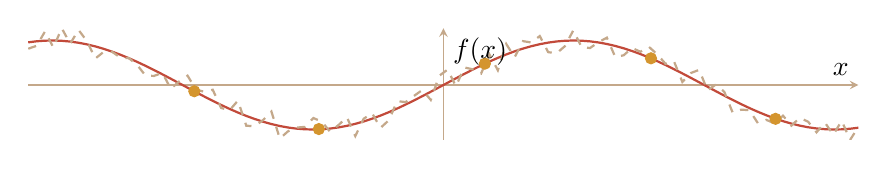
\begin{tikzpicture}
        \begin{axis}[
            width=\textwidth,
            height=3cm,
            xlabel={$x$},
            ylabel={$f(x)$},
            axis lines=middle,
            xtick=\empty,
            ytick=\empty,
            samples=50,
            domain=-5:5,
            enlargelimits=false,
            axis line style={draw=wp-muted},
            ticklabel style={font=\tiny}
        ]
        \addplot[wp-primary, thick, domain=-5:5, samples=100] {sin(deg(x))};
        \addplot[wp-muted, thick, dashed, domain=-5:5, samples=100] {sin(deg(x)) + 0.3*rand};
        \addplot[wp-accent, only marks, mark=*] coordinates {
            (-3, -0.14) (-1.5, -0.99) (0.5, 0.48) (2.5, 0.6) (4, -0.76)
        };
        \end{axis}
    \end{tikzpicture}
    \caption{Função seno (wp-primary), dados observados (wp-accent), e possível amostra de GP ajustado (wp-muted tracejado).}
\end{marginfigure}
\part{Ferramentas de Concentração, Incerteza e Decisão}

A Lei dos Grandes Números nos diz que médias convergem. O Teorema Central do Limite nos diz \textit{como} convergem --- a forma assintótica da distribuição. Mas estas são respostas assintóticas: valem quando $n \to \infty$. No mundo real, $n$ é finito, muitas vezes dolorosamente pequeno. Precisamos de ferramentas que funcionem para amostras finitas, que nos deem garantias não apenas no limite, mas para o tamanho de amostra que temos hoje.

Este capítulo reúne quatro famílias de ferramentas que lidam com essa realidade finita. As \textbf{desigualdades de concentração} nos permitem limitar a probabilidade de grandes desvios. O \textbf{bootstrap} e o \textbf{jackknife} nos permitem estimar a incerteza de estimadores sem assumir distribuições específicas. A \textbf{seleção de modelos} nos dá critérios para escolher entre hipóteses concorrentes sem overfitting. E a \textbf{teoria PAC} com a \textbf{dimensão VC} fornece as garantias mais profundas de generalização --- a promessa de que o aprendizado é possível.

Juntas, estas ferramentas formam o arsenal do estatístico e do cientista de dados moderno: o que fazer quando $n$ é finito, quando não conhecemos a distribuição, e quando precisamos decidir.

%===============================================================================
\section{Desigualdades de Concentração}
%===============================================================================

\paragraph{O problema da velocidade de convergência.}

A Lei dos Grandes Números é um dos teoremas mais belos da probabilidade: a média amostral converge para a esperança. Mas ela não nos diz \textit{quão rápido}. Se jogarmos uma moeda 100 vezes, quão próxima estará a proporção de caras de $1/2$? E se jogarmos 1000 vezes?

As \textbf{desigualdades de concentração} respondem a esta pergunta: elas fornecem cotas superiores para a probabilidade de que uma variável aleatória se desvie de seu valor esperado. São ferramentas de amostra finita --- valem para qualquer $n$, não apenas no limite.

A história começa com Pafnuty Chebyshev, em 1867. Seu aluno Andrey Markov refinou a desigualdade, e o trabalho foi estendido por Chernoff (1952), Hoeffding (1963), McDiarmid (1989), e muitos outros. Cada nova desigualdade aperta as cotas sob suposições mais específicas, revelando a tensão fundamental entre generalidade e precisão.

\paragraph{A desigualdade mais simples: Markov.}

Tudo começa com uma observação quase trivial:

\begin{thm}[Desigualdade de Markov]
    Seja $X \ge 0$ uma variável aleatória não-negativa. Para qualquer $a > 0$:
    \[
    P(X \ge a) \le \frac{\E[X]}{a}
    \]
\end{thm}

A prova é imediata: $\E[X] \ge \E[X \cdot \mathbbm{1}_{X \ge a}] \ge a \cdot P(X \ge a)$. Apesar de sua simplicidade, Markov é o ponto de partida de todas as desigualdades de concentração. Dela derivamos todas as outras.

Markov é fraca porque usa apenas o primeiro momento. Uma variável pode ter grande massa em valores extremos --- Markov ainda vale, mas a cota pode ser muito frouxa.

\paragraph{Usando a variância: Chebyshev.}

Se conhecemos a variância, podemos fazer melhor:

\begin{thm}[Desigualdade de Chebyshev, 1867]
    Seja $X$ uma variável aleatória com média $\mu$ e variância $\sigma^2$. Para qualquer $\epsilon > 0$:
    \[
    P(|X - \mu| \ge \epsilon) \le \frac{\sigma^2}{\epsilon^2}
    \]
\end{thm}

\begin{proof}
    Aplicamos Markov a $Y = (X - \mu)^2 \ge 0$: $P(|X-\mu| \ge \epsilon) = P(Y \ge \epsilon^2) \le \E[Y]/\epsilon^2 = \sigma^2/\epsilon^2$.
\end{proof}

Chebyshev já é mais informativa: nos diz que desvios grandes são improváveis \textit{proporcionalmente à variância}. Para a média amostral $\bar{X}_n$, temos $\Var(\bar{X}_n) = \sigma^2/n$, logo:
\[
P(|\bar{X}_n - \mu| \ge \epsilon) \le \frac{\sigma^2}{n\epsilon^2}
\]

A cota decai como $1/n$. Mas podemos fazer melhor.

\begin{exmp}
    Para uma moeda justa ($p = 1/2$), Chebyshev nos dá:
    \[
    P\left(\left|\frac{S_n}{n} - \frac12\right| \ge 0.1\right) \le \frac{1/4}{n \cdot 0.01} = \frac{25}{n}
    \]
    Para $n = 100$, a cota é $0.25$ --- verdadeira, mas conservadora. A probabilidade real é muito menor.
\end{exmp}

\paragraph{Chernoff: otimização via MGF.}

A ideia de Chernoff (1952) é elegante e poderosa: em vez de aplicar Markov diretamente a $X$, aplicamos a $e^{tX}$ para um parâmetro $t$ que escolhemos \textit{otimamente}:

\begin{thm}[Chernoff Bound]
    Para qualquer variável aleatória $X$ e qualquer $t > 0$:
    \[
    P(X \ge a) \le \frac{\E[e^{tX}]}{e^{ta}} = \exp\!\big(\log M_X(t) - ta\big)
    \]
    onde $M_X(t) = \E[e^{tX}]$ é a função geradora de momentos.
    Otimizamos sobre $t > 0$ para obter a cota mais apertada.
\end{thm}

Para somas de variáveis independentes, o Chernoff é particularmente poderoso. Se $X = \sum_{i=1}^n X_i$, com $X_i$ independentes, então $M_X(t) = \prod_i M_{X_i}(t)$, e a cota fatora.

\begin{thm}[Chernoff para Somas de Bernoulli]
    Sejam $X_1, \dots, X_n$ independentes com $X_i \in \{0,1\}$. Seja $\mu = \E[\sum X_i]$. Para $\delta > 0$:
    \[
    P\!\left(\sum_{i=1}^n X_i \ge (1+\delta)\mu\right) \le \left(\frac{e^\delta}{(1+\delta)^{1+\delta}}\right)^\mu
    \]
    E para $\delta \in (0,1)$:
    \[
    P\!\left(\sum_{i=1}^n X_i \le (1-\delta)\mu\right) \le \exp\!\left(-\frac{\mu\delta^2}{2}\right)
    \]
\end{thm}

A derivação ilustra o método geral. Para a cota superior, usamos $P(X \ge a) \le e^{-ta} \E[e^{tX}]$ com $X = \sum X_i$:
\[
\E[e^{tX}] = \prod_{i=1}^n \E[e^{tX_i}] = \prod_{i=1}^n (1 - p_i + p_i e^t) \le \prod_{i=1}^n \exp(p_i(e^t - 1)) = \exp\!\big(\mu(e^t - 1)\big)
\]
Otimizando $t = \log(1+\delta)$, obtemos a expressão acima.

A cota Chernoff decai \textit{exponencialmente} com $\mu$, muito mais rápido que o decaimento $1/n$ de Chebyshev.

\paragraph{Hoeffding: variáveis limitadas.}

Hoeffding (1963) generalizou Chernoff para variáveis limitadas, não apenas Bernoulli:

\begin{thm}[Desigualdade de Hoeffding]
    Sejam $X_1, \dots, X_n$ variáveis aleatórias independentes com $a_i \le X_i \le b_i$ quase certamente. Então, para qualquer $t > 0$:
    \[
    P\!\left(\big|\bar{X} - \E[\bar{X}]\big| \ge t\right) \le 2\exp\!\left(-\frac{2n^2 t^2}{\sum_{i=1}^n (b_i - a_i)^2}\right)
    \]
\end{thm}

A cota de Hoeffding não depende da distribuição --- apenas dos limites $a_i$ e $b_i$. Isto a torna universal e amplamente aplicável. Para variáveis em $[0,1]$, a cota simplifica para $2\exp(-2nt^2)$.

\begin{remark}
    Hoeffding é a ferramenta central para provar \textbf{limites de generalização} em aprendizado de máquina. Se o erro de cada exemplo é limitado (como na classificação 0-1), então o erro empírico converge para o erro esperado exponencialmente rápido.
\end{remark}

\paragraph{McDiarmid: diferenças limitadas.}

McDiarmid (1989) estendeu Hoeffding para funções de muitas variáveis, onde não há estrutura de soma:

\begin{thm}[Desigualdade de McDiarmid (Bounded Differences)]
    Seja $f: \mathcal{X}_1 \times \cdots \times \mathcal{X}_n \to \mathbb{R}$ uma função tal que, para todo $i$:
    \[
    \sup_{x_1, \dots, x_n, x_i'} |f(x_1, \dots, x_i, \dots, x_n) - f(x_1, \dots, x_i', \dots, x_n)| \le c_i
    \]
    (mudar a $i$-ésima coordenada altera $f$ em no máximo $c_i$). Se $X_1, \dots, X_n$ são independentes, então:
    \[
    P\!\left(f(X_1, \dots, X_n) - \E[f] \ge t\right) \le \exp\!\left(-\frac{2t^2}{\sum_i c_i^2}\right)
    \]
\end{thm}

McDiarmid é surpreendentemente geral. Ela se aplica a estimadores complexos onde a derivada em cada variável é limitada, incluindo medianas, quantis, e até mesmo riscos empíricos de classes de hipóteses.

\paragraph{Bennett: usando a variância.}

Chernoff e Hoeffding ignoram a variância das variáveis. Bennett (1962) propôs uma cota que incorpora a variância, produzindo limites mais apertados quando $\sigma^2$ é pequena:

\begin{thm}[Desigualdade de Bennett]
    Sejam $X_1, \dots, X_n$ independentes com $X_i \le b$ quase certamente, $\E[X_i] = 0$, e $\Var(X_i) = \sigma_i^2$. Seja $S_n = \sum X_i$ e $v = \sum \sigma_i^2$. Então, para qualquer $t > 0$:
    \[
    P(S_n \ge t) \le \exp\!\left(-\frac{v}{b^2} \, h\!\left(\frac{bt}{v}\right)\right)
    \]
    onde $h(u) = (1+u)\log(1+u) - u$.
\end{thm}

Quando $v$ é pequena (variância baixa), Bennett é significativamente mais apertada que Hoeffding.

\paragraph{Aplicações: por que isso importa.}

As desigualdades de concentração são a espinha dorsal de muitas garantias em aprendizado de máquina:

\begin{enumerate}
    \item \textbf{Limites de generalização para ERM}: Seja $\mathcal{H}$ uma classe de hipóteses finita. Pela desigualdade de Hoeffding e união de eventos:
    \[
    P\!\left(\max_{h \in \mathcal{H}} |R(h) - \hat{R}_n(h)| \ge t\right) \le 2|\mathcal{H}| \exp(-2nt^2)
    \]
    Segue que, com probabilidade $1-\delta$:
    \[
    R(\hat{h}) \le \hat{R}_n(\hat{h}) + \sqrt{\frac{\log|\mathcal{H}| + \log(2/\delta)}{2n}}
    \]
    O termo $\sqrt{\log|\mathcal{H}|/n}$ é a penalidade por complexidade.

    \item \textbf{Bandit algorithms (UCB)}: No problema do bandido multi-braço, o algoritmo UCB (Upper Confidence Bound) usa a desigualdade de Hoeffding para construir intervalos de confiança para cada braço, guiando a exploração.

    \item \textbf{Dimensão VC e convergência uniforme}: Para classes infinitas, substituímos $|\mathcal{H}|$ pela dimensão VC, obtendo limites de generalização uniformes. Expandiremos isto na Seção~6.4.
\end{enumerate}

\begin{remark}
    O padrão é sempre o mesmo: concentração + complexidade da classe = limite de generalização. A arte está em escolher a desigualdade de concentração adequada (Hoeffding para bounded, Bernstein/Bennett para variance-aware, McDiarmid para funções gerais) e a medida de complexidade correta (cardinalidade, VC-dim, Rademacher).
\end{remark}

%===============================================================================
\section{Bootstrap e Jackknife}
%===============================================================================

\paragraph{Duas ideias, um objetivo.}

Como estimamos a incerteza de um estimador quando não conhecemos a distribuição dos dados? Esta pergunta atormentou estatísticos por décadas. A resposta teórica --- a distribuição amostral de $\hat{\theta}$ --- é geralmente intratável. Duas técnicas surgiram para contornar este problema, ambas baseadas na mesma intuição: usar os próprios dados para simular o processo de amostragem.

O \textbf{jackknife} (facas de carta, no original inglês --- uma ferramenta versátil) foi inventado por Quenouille em 1949 para estimar o viés de estimadores. John Tukey, em 1958, percebeu que a mesma técnica podia estimar variâncias. O nome foi cunhado por Tukey: uma ferramenta multiuso, como um canivete suíço.

O \textbf{bootstrap} veio depois, proposto por Bradley Efron em 1979, em um artigo cujo título já era uma declaração de princípios: ``Bootstrap Methods: Another Look at the Jackknife''. O nome vem da expressão ``to pull oneself up by one's bootstraps'' --- levantar-se puxando os próprios cadarços --- pois o método usa os dados para inferir sobre os dados. Efron nos deu um mantra: ``Let the data speak for themselves.''

\paragraph{Jackknife: leave-one-out.}

A ideia do jackknife é simples e direta: removemos uma observação por vez e recalculamos o estimador, produzindo $n$ estimativas ``leave-one-out'' $\hat{\theta}_{(-i)}$.

\begin{defn}[Estimativas Jackknife]
    Seja $\hat{\theta}$ o estimador calculado com todos os $n$ dados, e $\hat{\theta}_{(-i)}$ o estimador calculado sem a $i$-ésima observação. A média das estimativas leave-one-out é:
    \[
    \hat{\theta}_{(\cdot)} = \frac{1}{n} \sum_{i=1}^n \hat{\theta}_{(-i)}
    \]
\end{defn}

O jackknife fornece estimadores de viés e variância:

\begin{align*}
    \widehat{\text{Bias}}_{\text{jack}} &= (n-1)(\hat{\theta}_{(\cdot)} - \hat{\theta}) \\
    \widehat{\Var}_{\text{jack}} &= \frac{n-1}{n} \sum_{i=1}^n (\hat{\theta}_{(-i)} - \hat{\theta}_{(\cdot)})^2
\end{align*}

O fator $(n-1)$ não é arbitrário. Ele emerge da expansão de Taylor do viés: se $\E[\hat{\theta}] = \theta + b/n + O(1/n^2)$, então $\E[\widehat{\text{Bias}}_{\text{jack}}] = b/n + O(1/n^2)$.

\begin{exmp}[Jackknife para a média]
    Para $\hat{\theta} = \bar{x}$, temos $\hat{\theta}_{(-i)} = (n\bar{x} - x_i)/(n-1)$. A média destas é $\bar{x}$ (pois $\sum_i \hat{\theta}_{(-i)} = n\bar{x}$). Logo $\widehat{\text{Bias}}_{\text{jack}} = 0$ --- a média é não-viesada. A variância jackknife recupera $\sigma^2/n$ exatamente.
\end{exmp}

\begin{remark}
    O jackknife é \textbf{determinístico}: dado um conjunto de dados, produz sempre o mesmo resultado. Não há aleatoriedade envolvida --- diferentemente do bootstrap. Sua principal limitação é que pode falhar para estimadores não-suaves, como a mediana.
\end{remark}

\paragraph{Bootstrap: a ideia revolucionária.}

O bootstrap de Efron é conceptualmente simples e computacionalmente intensivo:

\begin{enumerate}
    \item Temos uma amostra $X_1, \dots, X_n$ de uma distribuição desconhecida $F$.
    \item A \textbf{distribuição empírica} $\hat{F}_n$ atribui massa $1/n$ a cada $X_i$.
    \item Amostramos $n$ pontos \textbf{com reposição} de $\hat{F}_n$ --- esta é uma \textbf{amostra bootstrap} $X_1^*, \dots, X_n^*$.
    \item Calculamos $\hat{\theta}^*$ nesta amostra bootstrap.
    \item Repetimos $B$ vezes (tipicamente $B = 1000$ ou $B = 10000$).
\end{enumerate}

A distribuição empírica dos $\hat{\theta}_b^*$ aproxima a distribuição amostral de $\hat{\theta}$.

\begin{defn}[Bootstrap não-paramétrico]
    Para $b = 1, \dots, B$:
    \begin{itemize}
        \item Amostre $X_1^*, \dots, X_n^* \sim \hat{F}_n$ (com reposição).
        \item Compute $\hat{\theta}_b^* = \hat{\theta}(X_1^*, \dots, X_n^*)$.
    \end{itemize}
    O conjunto $\{\hat{\theta}_1^*, \dots, \hat{\theta}_B^*\}$ é uma amostra da \textbf{distribuição bootstrap} de $\hat{\theta}$.
\end{defn}

Existe também o \textbf{bootstrap paramétrico}: se assumimos que $X_i \sim F_\theta$ para alguma família paramétrica, estimamos $\hat{\theta}$ e amostramos de $F_{\hat{\theta}}$. Isto é útil quando o modelo paramétrico é confiável e queremos incorporar essa estrutura.

\paragraph{Por que o bootstrap funciona.}

A justificativa teórica é elegantemente simples: a distribuição empírica $\hat{F}_n$ converge para a verdadeira distribuição $F$ (pelo teorema de Glivenko-Cantelli). Portanto, amostrar de $\hat{F}_n$ é aproximadamente o mesmo que amostrar de $F$. Esta aproximação melhora com $n$.

Mais formalmente, sob condições de regularidade, a distribuição bootstrap de $\sqrt{n}(\hat{\theta}^* - \hat{\theta})$ converge para a mesma distribuição limite de $\sqrt{n}(\hat{\theta} - \theta)$. O bootstrap é \textbf{consistente}.

\begin{remark}
    O bootstrap é, ele próprio, um estimador de Monte Carlo. Estamos usando Monte Carlo para aproximar a distribuição amostral de $\hat{\theta}$ --- um bootstrap dentro de um Monte Carlo. A conexão é profunda: toda vez que usamos simulação para estimar uma quantidade determinística, estamos fazendo Monte Carlo.
\end{remark}

\paragraph{Intervalos de confiança bootstrap.}

Existem múltiplas formas de construir intervalos de confiança via bootstrap:

\begin{itemize}
    \item \textbf{Percentil bootstrap}: Usa os percentis $(\alpha/2)$ e $(1-\alpha/2)$ da distribuição bootstrap:
    \[
    [\hat{\theta}_{(\alpha/2)}^*, \; \hat{\theta}_{(1-\alpha/2)}^*]
    \]
    Simples, mas pode ter viés.

    \item \textbf{BCa (Bias-Corrected and Accelerated)}: Correção de viés e assimetria. Mais preciso que o percentil, mas computacionalmente mais caro. É o método recomendado por Efron.

    \item \textbf{Bootstrap-t}: Usa a estatística $t = (\hat{\theta} - \theta)/\widehat{\text{SE}}(\hat{\theta})$ e aproxima sua distribuição via bootstrap. Requer um estimador de erro padrão para cada amostra bootstrap (bootstrap duplo).
\end{itemize}

\begin{exmp}[Bootstrap para a mediana]
    A mediana é um estimador não-suave --- o jackknife falha. O bootstrap, porém, funciona bem. Dados $n = 50$ pontos de uma distribuição assimétrica, o bootstrap nos dá uma distribuição para a mediana amostral, com intervalos de confiança que refletem a incerteza real.
\end{exmp}

\paragraph{Limitações.}

O bootstrap não é uma bala de prata:

\begin{itemize}
    \item \textbf{Custo computacional}: Para $B = 10000$ iterações e $n$ grande, o custo pode ser proibitivo. O bootstrap paramétrico e o bootstrap residual (para regressão) são alternativas mais leves.
    \item \textbf{Amostras pequenas}: Para $n$ muito pequeno (digamos $n < 20$), as amostras bootstrap são degeneradas (muitas repetições dos mesmos pontos). A aproximação $\hat{F}_n \approx F$ é pobre.
    \item \textbf{Estatísticas extremas}: O bootstrap pode falhar para máximos, mínimos, ou estimadores não-consistentes (ex: estimador de correlação quando a correlação verdadeira é $\pm 1$).
    \item \textbf{Dependência}: O bootstrap padrão assume i.i.d. Para séries temporais, precisamos de versões modificadas (block bootstrap).
\end{itemize}

\paragraph{Bootstrap em aprendizado de máquina: bagging.}

A aplicação mais influente do bootstrap em ML é o \textbf{bagging} (Bootstrap Aggregating), proposto por Leo Breiman em 1996. A ideia: treinar o mesmo modelo em $B$ amostras bootstrap dos dados, e combinar as previsões por média (regressão) ou votação (classificação):

\[
\hat{f}_{\text{bag}}(x) = \frac{1}{B} \sum_{b=1}^B \hat{f}_b^*(x)
\]

O bagging reduz a \textbf{variância} mantendo o viés aproximadamente constante. É particularmente eficaz para modelos de alta variância como árvores de decisão --- precisamente por isso, o classificador \textbf{random forest} (que combina bagging com seleção aleatória de features) é um dos métodos mais bem-sucedidos da história do ML.

\begin{remark}
    Bagging funciona porque a correlação entre modelos treinados em diferentes amostras bootstrap é menor que 1. Se os $B$ modelos fossem independentes, a variância da média seria $\sigma^2/B$. Na prática, a correlação reduz o ganho, mas a redução de variância ainda é substancial.
\end{remark}

%===============================================================================
\section{Seleção e Comparação de Modelos}
%===============================================================================

\paragraph{O dilema do modelador.}

Dado um conjunto de dados, podemos ajustar modelos de complexidade crescente: regressão linear, polinômios de grau 2, 3, \dots, 20. O polinômio de grau 20 vai ajustar os dados perfeitamente --- mas vai prever horrivelmente novos dados. Este é o paradoxo central da modelagem estatística: modelos mais complexos ajustam melhor os dados observados, mas generalizam pior.

Como escolher o modelo certo? A resposta envolve equilibrar ajuste e complexidade, e a literatura nos oferece múltiplas ferramentas.

\paragraph{O princípio da Navalha de Occam.}

Guilherme de Occam, frade franciscano do século XIV, enunciou o princípio: ``Entia non sunt multiplicanda praeter necessitatem'' --- as entidades não devem ser multiplicadas além da necessidade. Em termos estatísticos: entre dois modelos com ajuste similar, prefira o mais simples.

Esta intuição, porém, não nos dá um critério \textit{quantitativo}. Precisamos de métricas que traduzam ``simplicidade'' em números.

\paragraph{Validação cruzada.}

A abordagem mais direta: em vez de avaliar o modelo nos mesmos dados usados para treinar, separe dados para teste. A \textbf{validação cruzada} (cross-validation) leva esta ideia ao extremo.

\begin{defn}[$k$-fold Cross-Validation]
    \hfill
    \begin{enumerate}
        \item Particione os dados em $k$ subconjuntos (folds) de tamanhos aproximadamente iguais.
        \item Para cada fold $i = 1, \dots, k$:
        \begin{itemize}
            \item Treine o modelo nos outros $k-1$ folds.
            \item Avalie o erro no fold $i$ (erro de validação).
        \end{itemize}
        \item O erro de CV é a média dos $k$ erros de validação.
    \end{enumerate}
\end{defn}

Dois casos extremos merecem atenção:

\begin{itemize}
    \item \textbf{Leave-one-out (LOO-CV)}: $k = n$. Treinamos em $n-1$ pontos, testamos no ponto deixado de fora. É aproximadamente não-viesado (treinamos em quase todos os dados), mas tem alta variância (cada modelo é treinado em conjuntos quase idênticos, produzindo estimativas correlacionadas). Custo computacional $O(n)$ (para modelos que podem ser atualizados incrementalmente).

    \item \textbf{$k$-fold com $k=5$ ou $k=10$}: compromisso prático. $k=5$ tem viés ligeiramente maior que LOO, mas variância menor. $k=10$ é próximo de LOO em viés, com custo $10\times$ o treinamento.
\end{itemize}

\begin{remark}
    A escolha de $k$ reflete um \textbf{bias-variance tradeoff} na própria validação cruzada: $k$ pequeno $\to$ mais viés (treinamos com menos dados), $k$ grande $\to$ mais variância (folds muito sobrepostos). O valor $k=5$ ou $k=10$ funciona bem na prática (Breiman, 1996; Kohavi, 1995).
\end{remark}

Para problemas de classificação, a \textbf{validação cruzada estratificada} preserva a proporção de classes em cada fold --- crucial quando as classes são desbalanceadas.

\paragraph{Critérios de informação: AIC e BIC.}

Quando a validação cruzada é computacionalmente proibitiva (ou quando queremos um critério analítico), recorremos a critérios de informação baseados na verossimilhança.

\begin{defn}[AIC --- Akaike Information Criterion, 1974]
    \[
    \text{AIC} = -2\log \hat{L} + 2k
    \]
    onde $\hat{L}$ é a verossimilhança maximizada e $k$ o número de parâmetros do modelo.
\end{defn}

A derivação de Akaike é bela. Sob condições de regularidade, a divergência de KL entre o modelo verdadeiro $g$ e o modelo estimado $f_{\hat{\theta}}$ pode ser aproximada. O termo $-2\log \hat{L}$ mede o ajuste; o termo $2k$ penaliza a complexidade. Minimizar AIC é aproximadamente equivalente a minimizar a divergência de KL esperada.

\begin{defn}[BIC --- Bayesian Information Criterion, Schwarz, 1978]
    \[
    \text{BIC} = -2\log \hat{L} + k\log n
    \]
    onde $n$ é o tamanho da amostra.
\end{defn}

A derivação de BIC é bayesiana: aproximamos a verossimilhança marginal (evidência) por Laplace:
\[
p(\mathcal{D}) = \int p(\mathcal{D} \mid \theta) \, p(\theta) \, d\theta \approx \hat{L} \cdot (2\pi)^{k/2} |\mathcal{I}(\hat{\theta})|^{-1/2} \cdot p(\hat{\theta})
\]
Tomando $-2\log$ e ignorando termos constantes, obtemos BIC. O BIC aproxima o \textbf{fator de Bayes} entre modelos, permitindo comparação bayesiana sem especificar priors.

\begin{remark}
    A diferença entre AIC e BIC é reveladora:
    \begin{itemize}
        \item AIC minimiza erro de \textbf{predição} (é assintoticamente eficiente: escolhe o modelo com menor erro de predição esperado).
        \item BIC identifica o \textbf{modelo verdadeiro} se ele estiver na classe considerada (é consistente: a probabilidade de escolher o modelo correto tende a 1).
        \item BIC penaliza complexidade mais fortemente ($k\log n$ vs. $2k$). Para $n > 8$, $\log n > 2$.
    \end{itemize}
    A escolha entre AIC e BIC depende do objetivo: predição ou inferência causal.
\end{remark}

\paragraph{WAIC: a versão Bayesiana completa.}

Watanabe (2010) propôs o WAIC (Watanabe-Akaike Information Criterion), uma generalização totalmente bayesiana:

\[
\text{WAIC} = -2 \sum_{i=1}^n \log \E_{\theta \mid \mathcal{D}}[p(y_i \mid \theta)] + 2 \sum_{i=1}^n \Var_{\theta \mid \mathcal{D}}[\log p(y_i \mid \theta)]
\]

O primeiro termo é a log-verossimilhança preditiva pontual; o segundo penaliza a complexidade medida pela variabilidade das predições. WAIC é particularmente útil para modelos com priors informativas e posteriores complexas, onde AIC e BIC são inadequados.

\paragraph{Minimum Description Length (MDL).}

Uma perspectiva radicalmente diferente vem da teoria da informação. O princípio MDL (Rissanen, 1978) diz: o melhor modelo é aquele que minimiza o comprimento total da descrição dos dados mais o modelo.

\[
\text{MDL} = L(\text{modelo}) + L(\text{dados} \mid \text{modelo})
\]

A conexão com a navalha de Occam é direta: modelos simples têm descrição curta; modelos que se ajustam bem aos dados também têm descrição curta dos resíduos. O comprimento de descrição ótimo é, idealmente, a \textbf{complexidade de Kolmogorov} (o comprimento do programa mais curto que gera os dados), que é incomputável. Na prática, usamos aproximações como o \textbf{two-part MDL} ou o \textbf{normalized maximum likelihood}.

\begin{remark}
    Surpreendentemente, MDL coincide com BIC em muitos casos. Mas a filosofia é diferente: MDL não assume que existe um ``modelo verdadeiro''. É uma teoria de aprendizado sem pressupostos ontológicos.
\end{remark}

\paragraph{Testes de hipótese para comparação de modelos.}

Quando dois modelos são \textbf{aninhados} (um é caso particular do outro), podemos usar testes formais:

\begin{itemize}
    \item \textbf{Teste da razão de verossimilhanças}: $D = -2\log(L_{\text{simples}} / L_{\text{complexo}})$. Sob $H_0$ (modelo simples é suficiente), $D \sim \chi^2_{\Delta k}$, onde $\Delta k$ é a diferença no número de parâmetros.
    \item \textbf{ANOVA} (regressão linear): Compara a redução na soma de quadrados ao custo em graus de liberdade.
\end{itemize}

\begin{exmp}[Seleção de grau polinomial]
    Ajustamos polinômios de graus 1 a 10 a $n = 50$ pontos. O erro de treino cai monotonicamente. O erro de teste (ou CV) tipicamente tem mínimo em grau 3 ou 4. AIC e BIC geralmente concordam com CV, mas BIC tende a escolher modelos ligeiramente mais simples.
\end{exmp}

\paragraph{Recomendações práticas.}

\begin{enumerate}
    \item \textbf{Se você tem dados suficientes}: use validação cruzada (k=5 ou k=10) com múltiplas repetições. É o método mais robusto e menos sujeito a suposições.
    \item \textbf{Se CV é muito cara}: use AIC para predição, BIC para seleção de variáveis.
    \item \textbf{Se o modelo é Bayesiano}: use WAIC ou leave-one-out (LOO) via aproximação de Pareto (Vehtari et al., 2017).
    \item \textbf{Sempre reporte incerteza}: erros de CV têm variância. Intervalos de confiança para o erro de CV são importantes.
\end{enumerate}

%===============================================================================
\section{Teoria da Aprendizagem PAC e Dimensão VC (Expansão)}
%===============================================================================

\paragraph{A pergunta fundamental.}

Por que o aprendizado de máquina funciona? Dado um conjunto finito de exemplos, por que um modelo consegue prever corretamente em exemplos nunca vistos? Esta é a pergunta mais profunda da teoria da aprendizagem computacional --- e sua resposta é o que chamamos de \textbf{teoria PAC}.

\paragraph{PAC Learning (Valiant, 1984).}

Leslie Valiant, em seu artigo seminal de 1984, propôs um arcabouço para responder a esta pergunta. A ideia: um conceito é \textbf{aprendível} se existe um algoritmo que, com alta probabilidade, produz uma hipótese com baixo erro, desde que receba exemplos suficientes.

\begin{defn}[PAC Learning]
    Uma classe de conceitos $\mathcal{C}$ sobre $\mathcal{X}$ é \textbf{PAC-aprendível} se existe um algoritmo $A$ e uma função polinomial $m(\cdot, \cdot)$ tal que, para qualquer $\epsilon > 0$ (precisão), $\delta > 0$ (confiança), e qualquer distribuição $D$ sobre $\mathcal{X} \times \{0,1\}$, se $A$ receber $n \ge m(\epsilon, \delta)$ exemplos i.i.d., então:
    \[
    P_{S \sim D^n}\big(R(A(S)) \le \epsilon\big) \ge 1 - \delta
    \]
    onde $R(h) = P_{(x,y) \sim D}(h(x) \neq y)$ é o risco verdadeiro (erro de generalização).
\end{defn}

O nome ``Probably Approximately Correct'' captura a essência: com probabilidade $1-\delta$ (Probably), o erro é no máximo $\epsilon$ (Approximately Correct). A função $m(\epsilon, \delta)$ é a \textbf{complexidade amostral} --- quantos exemplos são necessários.

Para classes finitas $\mathcal{H}$, vimos que a complexidade amostral é $O(\log(|\mathcal{H}|/\delta)/\epsilon^2)$ via Hoeffding + union bound. Mas e para classes infinitas?

\paragraph{Dimensão VC (Vapnik-Chervonenkis).}

Em 1971, os matemáticos russos Vladimir Vapnik e Alexey Chervonenkis publicaram um resultado que se tornaria o coração da teoria estatística do aprendizado: uma medida da capacidade de uma classe de hipóteses que permite limites de generalização para classes infinitas.

\begin{defn}[Dimensão VC]
    A dimensão VC de uma classe de hipóteses $\mathcal{H}$, denotada $\text{VC}(\mathcal{H})$, é o maior número $m$ tal que existe um conjunto de $m$ pontos em $\mathcal{X}$ que pode ser \textbf{destruído} (shattered) por $\mathcal{H}$.

    Um conjunto $\{x_1, \dots, x_m\}$ é destruído se, para qualquer atribuição de rótulos $\{y_1, \dots, y_m\} \in \{0,1\}^m$, existe $h \in \mathcal{H}$ com $h(x_i) = y_i$ para todo $i$.
\end{defn}

Se $\mathcal{H}$ pode destruir conjuntos arbitrariamente grandes, $\text{VC}(\mathcal{H}) = \infty$, e a classe não é PAC-aprendível. Caso contrário, a dimensão VC finita é condição necessária e suficiente para a aprendibilidade PAC.

\begin{exmp}[Exemplos clássicos de dimensão VC]
    \hfill
    \begin{itemize}
        \item \textbf{Intervalos em $\mathbb{R}$}: A classe dos intervalos $[a,b]$ pode destruir 2 pontos, mas não 3 (não podemos rotular o ponto do meio como 0 e os extremos como 1). $\text{VC} = 2$.

        \item \textbf{Classificadores lineares em $\mathbb{R}^d$}: A classe $\{x \mapsto \sign(w^T x + b) : w \in \mathbb{R}^d, b \in \mathbb{R}\}$ tem $\text{VC} = d+1$. Em $\mathbb{R}^2$, conseguimos destruir 3 pontos (não-colineares) mas não 4.

        \item \textbf{Redes neurais}: Para uma rede feedforward com $W$ pesos e $U$ neurônios, usando a função de ativação sign, a dimensão VC é $O(W \log(UW))$. Para ReLU, os limites são mais complexos, mas a dimensão VC pode ser muito grande, explicando o poder expressivo e o risco de overfitting.
    \end{itemize}
\end{exmp}

\paragraph{O limite fundamental de generalização.}

Vapnik e Chervonenkis provaram o resultado central:

\begin{thm}[Limite VC de Generalização]
    Com probabilidade $1 - \delta$, para toda $h \in \mathcal{H}$:
    \[
    R(h) \le \hat{R}_n(h) + \mathcal{O}\!\left(\sqrt{\frac{\text{VC}(\mathcal{H})}{n} \log\frac{n}{\text{VC}(\mathcal{H})} + \frac{1}{n}\log\frac{1}{\delta}}\right)
    \]
\end{thm}

A intuição é clara: o erro de generalização é limitado pelo erro empírico mais um termo que cresce com a razão entre a capacidade da classe (VC-dim) e o número de exemplos. Para que o aprendizado seja possível, precisamos que $n \gg \text{VC}(\mathcal{H})$.

\begin{remark}
    Este limite é \textbf{independente da distribuição} --- vale para qualquer $D$. Esta universalidade é uma força (robustez) e uma fraqueza (limites pessimistas). Na prática, limites dependentes da distribuição (como Rademacher) são mais apertados.
\end{remark}

\paragraph{Minimização de Risco Estrutural (SRM).}

Vapnik propôs uma estratégia para escolher a complexidade da classe: em vez de minimizar apenas o risco empírico, minimizamos o \textbf{limite superior} do risco verdadeiro.

Dada uma hierarquia de classes $\mathcal{H}_1 \subset \mathcal{H}_2 \subset \cdots \subset \mathcal{H}_k$ com $\text{VC}(\mathcal{H}_1) \le \text{VC}(\mathcal{H}_2) \le \cdots$, escolhemos $h \in \mathcal{H}_i$ que minimiza:
\[
\hat{R}_n(h) + \text{penalidade}(\text{VC}(\mathcal{H}_i), n, \delta)
\]

SRM é uma formalização da navalha de Occam: trocamos ajuste por complexidade de forma otimizada.

\paragraph{Rademacher complexity.}

A dimensão VC é uma medida \textbf{puramente combinatória} da capacidade de uma classe --- não depende da distribuição dos dados. A \textbf{complexidade de Rademacher} é uma alternativa \textbf{dependente dos dados} que produz limites mais apertados.

\begin{defn}[Complexidade de Rademacher]
    Seja $\mathcal{F}$ uma classe de funções $f: \mathcal{X} \to \mathbb{R}$. Sejam $\sigma_1, \dots, \sigma_n$ variáveis i.i.d. com $P(\sigma_i = 1) = P(\sigma_i = -1) = 1/2$ (variáveis de Rademacher). A \textbf{complexidade de Rademacher empírica} é:
    \[
    \hat{\mathcal{R}}_n(\mathcal{F}) = \E_\sigma\!\left[\sup_{f \in \mathcal{F}} \frac{1}{n} \sum_{i=1}^n \sigma_i f(X_i)\right]
    \]
    E a \textbf{complexidade de Rademacher esperada} é $\mathcal{R}_n(\mathcal{F}) = \E_X[\hat{\mathcal{R}}_n(\mathcal{F})]$.
\end{defn}

A interpretação: $\mathcal{R}_n(\mathcal{F})$ mede quão bem $\mathcal{F}$ pode se ajustar a ruído aleatório. Se $\mathcal{F}$ é rica, existe $f$ que se correlaciona bem com $\sigma$ puramente ao acaso.

\begin{thm}[Limite de Rademacher]
    Com probabilidade $1 - \delta$, para toda $f \in \mathcal{F}$ com $0 \le f(x) \le 1$:
    \[
    \E[f] \le \frac{1}{n} \sum_{i=1}^n f(X_i) + 2\mathcal{R}_n(\mathcal{F}) + \sqrt{\frac{\log(1/\delta)}{2n}}
    \]
\end{thm}

Limites via Rademacher têm várias vantagens:
\begin{itemize}
    \item Dependem dos dados (através de $X_i$) --- podem ser mais apertados que VC.
    \item Conectam-se naturalmente a margens, normas, e regularização.
    \item Generalizam para classes ricas como redes neurais (via normas espectrais, normas de caminho, etc.).
\end{itemize}

\begin{exmp}[Rademacher e margens]
    Para classificadores lineares com norma limitada $\|w\| \le B$ e dados em bola de raio $R$, a complexidade de Rademacher é $\mathcal{R}_n(\mathcal{F}) \le BR/\sqrt{n}$. O termo $BR/\sqrt{n}$ substitui $\sqrt{\text{VC-dim}/n}$ e é independente da dimensão $d$ --- o que explica por que SVMs funcionam bem em espaços de alta dimensão.
\end{exmp}

\paragraph{No-Free-Lunch: por que precisamos de viés indutivo.}

O teorema \textbf{No-Free-Lunch} (Wolpert, 1996) é um resultado profundo e frequentemente mal interpretado. Ele diz: nenhum algoritmo de aprendizado é intrinsecamente melhor que qualquer outro quando consideramos \textit{todos} os problemas possíveis.

Mais formalmente: para qualquer algoritmo $A_1$ e $A_2$, existe uma distribuição $D$ onde $A_1$ supera $A_2$, e outra onde $A_2$ supera $A_1$, quando o desempenho é médio sobre todas as distribuições.

A consequência: \textbf{viés indutivo é necessário}. Não existe aprendizado sem suposições. A arte do ML está em escolher suposições (viés) que sejam apropriadas para o problema em mãos --- seja ele visão computacional, processamento de linguagem natural, ou bioinformática.

\begin{remark}
    O No-Free-Lunch não diz que todos os algoritmos são igualmente bons na prática. Diz que não há almoço grátis \textit{universalmente}. Na prática, o mundo real tem estrutura --- suavidade, periodicidade, hierarquia --- e bons algoritmos exploram essa estrutura.
\end{remark}

\paragraph{Double descent: o fenômeno moderno.}

Nas últimas décadas, um fenômeno surpreendente foi observado em redes neurais profundas. A curva tradicional de bias-variance prevê que o erro de teste decresce, atinge um mínimo, e então cresce com a complexidade (overfitting). Mas em modelos superparametrizados (com mais parâmetros que exemplos), o erro de teste \textit{decresce novamente} após o ponto de interpolação.

\begin{defn}[Double Descent]
    O \textbf{fenômeno do double descent} (Belkin et al., 2019) descreve a curva de erro de teste como função da complexidade do modelo:
    \begin{itemize}
        \item Fase 1 (subparametrizada): erro decresce com a complexidade.
        \item Pico: no \textbf{limiar de interpolação} (número de parâmetros $\approx n$), o erro atinge um pico. O modelo pode ajustar os dados perfeitamente, mas generaliza mal.
        \item Fase 2 (superparametrizada): erro decresce novamente. Modelos com muitos parâmetros --- até mesmo interpolando perfeitamente os dados --- podem generalizar bem.
    \end{itemize}
\end{defn}

Este fenômeno desafia a sabedoria convencional de que modelos complexos sempre overfitam. Ele está conectado à \textbf{descoberta de que redes neurais profundas podem generalizar apesar de memorizar os dados de treino} (Zhang et al., 2017). A compreensão teórica do double descent envolve o kernel do modelo, a relação entre parâmetros e dados, e a \textbf{benign overfitting} (Bartlett et al., 2020).

\begin{remark}
    O double descent reconcilia a teoria clássica (VC-dim, bias-variance) com a prática moderna de deep learning. Na região superparametrizada, o limite de VC é enorme (possivelmente infinito), mas o modelo ainda generaliza --- porque o algoritmo de otimização (SGD) implicitamente regulariza a solução, escolhendo hipóteses de ``baixa complexidade'' dentro da classe gigantesca.
\end{remark}

A teoria da aprendizagem PAC e a dimensão VC nos dão as garantias mais fundamentais: condições sob as quais o aprendizado é possível, e limites que quantificam o esforço necessário. Mas a história não termina aqui. A cada década, novos fenômenos --- double descent, benign overfitting, neural tangent kernels --- desafiam e expandem nossa compreensão. O que não muda é a pergunta central: \textit{quando e por que o aprendizado a partir de dados finitos é possível?}


%%%%%%%%%%%%%%%%%%%%%%%%%%%%%%%%%%%%%%%%%%%%%%%%%%%%%%%%%%%%%%%%%%%%%%%%%%%%%%%%
% PART VII: DO PROBABILÍSTICO AO APRENDIZADO DE MÁQUINA
%%%%%%%%%%%%%%%%%%%%%%%%%%%%%%%%%%%%%%%%%%%%%%%%%%%%%%%%%%%%%%%%%%%%%%%%%%%%%%%%

\part{Do Probabilístico ao Aprendizado de Máquina}

\section{Estimadores e Suas Propriedades}

\begin{defn}[Estimador]
    Um \textbf{estimador} $\hat{\theta}_n$ de um parâmetro $\theta$ é uma função dos
    dados $X_1, \dots, X_n$:
    \[
    \hat{\theta}_n = g(X_1, \dots, X_n)
    \]
\end{defn}

\begin{defn}[Propriedades de Estimadores]
    \begin{itemize}
        \item \textbf{Não-viesado}: $\E[\hat{\theta}_n] = \theta$.
        \item \textbf{Consistente}: $\hat{\theta}_n \xrightarrow{P} \theta$ quando
        $n \to \infty$.
        \item \textbf{Eficiente}: $\Var(\hat{\theta}_n)$ é mínimo entre todos os
        estimadores não-viesados (atinge o limite de Cramér--Rao).
        \item \textbf{Assintoticamente normal}: $\sqrt{n}(\hat{\theta}_n - \theta) \xrightarrow{d} \mathcal{N}(0, \sigma^2_\theta)$.
    \end{itemize}
\end{defn}

\subsection{Maximum Likelihood Estimation (MLE)}

O princípio da máxima verossimilhança é simples: escolha os parâmetros que tornam os
dados observados mais prováveis.

\begin{defn}[Função de Verossimilhança]
    Dados i.i.d. $X_1, \dots, X_n \sim p(x \mid \theta)$, a função de verossimilhança é:
    \[
    L(\theta) = \prod_{i=1}^n p(x_i \mid \theta)
    \]
    O estimador de máxima verossimilhança (MLE) é:
    \[
    \hat{\theta}_{\text{MLE}} = \argmax_\theta L(\theta) = \argmax_\theta \sum_{i=1}^n \log p(x_i \mid \theta)
    \]
\end{defn}

\begin{exmp}[MLE para Bernoulli]
    Se $X_i \sim \Bern(p)$, i.i.d.:
    \[
    L(p) = \prod_{i=1}^n p^{x_i} (1-p)^{1-x_i}
    \]
    \[
    \ell(p) = \sum x_i \log p + (n - \sum x_i) \log(1-p)
    \]
    \[
    \frac{d\ell}{dp} = \frac{\sum x_i}{p} - \frac{n - \sum x_i}{1-p} = 0 \implies \hat{p} = \frac{1}{n}\sum x_i
    \]
    O MLE é a média amostral --- a frequência relativa de sucessos.
\end{exmp}

\begin{prop}[Propriedades Assintóticas do MLE]
    Sob condições de regularidade:
    \begin{enumerate}
        \item Consistência: $\hat{\theta}_{\text{MLE}} \xrightarrow{P} \theta$
        \item Normalidade assintótica: $\sqrt{n}(\hat{\theta}_{\text{MLE}} - \theta) \xrightarrow{d} \mathcal{N}(0, I(\theta)^{-1})$
        onde $I(\theta) = -\E[\frac{\partial^2 \log p(x\mid\theta)}{\partial\theta^2}]$ é a
        \textbf{informação de Fisher}.
        \item Eficiência assintótica: atinge o limite de Cramér--Rao.
    \end{enumerate}
\end{prop}

A conexão com aprendizado de máquina: o treinamento de redes neurais é MLE.
Minimizar a cross-entropy loss é maximizar a log-verossimilhança sob uma distribuição
categórica (classificação). Minimizar o erro quadrático (MSE) é maximizar a
log-verossimilhança sob uma distribuição Gaussiana (regressão).

\subsection{Maximum A Posteriori (MAP)}

O estimador MAP incorpora conhecimento prévio via uma distribuição a priori:

\[
\hat{\theta}_{\text{MAP}} = \argmax_\theta p(\theta \mid \mathcal{D}) = \argmax_\theta \left[\log p(\mathcal{D} \mid \theta) + \log p(\theta) \right]
\]

\begin{exmp}[MAP com priori Gaussiana]
    Seja $p(\theta) = \mathcal{N}(0, \sigma_0^2)$ e o modelo de verossimilhança Gaussiana.
    Então:
    \[
    \log p(\theta \mid \mathcal{D}) = -\frac{1}{2\sigma^2}\sum (y_i - f_\theta(x_i))^2 - \frac{1}{2\sigma_0^2}\|\theta\|^2 + \text{const}
    \]
    Isto é exatamente a regularização $L_2$ (weight decay)! O termo de regularização
    $\lambda\|\theta\|^2$ corresponde a uma priori Gaussiana com $\lambda = \sigma^2/\sigma_0^2$.
    A regularização $L_1$ (Lasso) corresponde a uma priori Laplace.
\end{exmp}

\subsection{Inferência Bayesiana}
\label{sec:bayesian}

Na inferência bayesiana completa, não nos contentamos com uma estimativa pontual
$\hat{\theta}$. Calculamos a distribuição a posteriori completa:

\[
p(\theta \mid \mathcal{D}) = \frac{p(\mathcal{D} \mid \theta) p(\theta)}{p(\mathcal{D})}
\]

A predição para um novo ponto $x^*$ é feita integrando sobre a incerteza dos parâmetros:

\[
p(y^* \mid x^*, \mathcal{D}) = \int p(y^* \mid x^*, \theta) p(\theta \mid \mathcal{D}) d\theta
\]

Isto é chamado de \textbf{inferência preditiva bayesiana}. Ela naturalmente quantifica
a incerteza, mas a integral é frequentemente intratável --- daí a necessidade de MCMC
e aproximações variacionais.

\section{Bias-Variance Tradeoff}

\begin{defn}[Decomposição Bias-Variância]
    Para um estimador $\hat{f}(x)$ de uma função alvo $f(x)$ com ruído $\varepsilon$
    ($y = f(x) + \varepsilon$, $\E[\varepsilon] = 0$, $\Var(\varepsilon) = \sigma^2_\varepsilon$):
    \[
    \E[(y - \hat{f}(x))^2] = \underbrace{(\E[\hat{f}(x)] - f(x))^2}_{\text{Bias}^2}
    + \underbrace{\Var(\hat{f}(x))}_{\text{Variância}}
    + \underbrace{\sigma^2_\varepsilon}_{\text{Ruído irredutível}}
    \]
\end{defn}

\begin{proof}
    \begin{align*}
        \E[(y - \hat{f})^2] &= \E[(f + \varepsilon - \hat{f})^2] \\
        &= \E[(f - \hat{f})^2] + \E[\varepsilon^2] + 2\E[(f - \hat{f})\varepsilon] \\
        &= \E[(f - \E[\hat{f}] + \E[\hat{f}] - \hat{f})^2] + \sigma^2_\varepsilon \\
        &= (f - \E[\hat{f}])^2 + \E[(\E[\hat{f}] - \hat{f})^2] + \sigma^2_\varepsilon \\
        &= \text{Bias}^2 + \text{Variância} + \text{Ruído}
    \end{align*}
\end{proof}

O tradeoff é fundamental: modelos simples têm alto bias (subajuste) mas baixa variância;
modelos complexos têm baixo bias mas alta variância (sobreajuste). O objetivo é encontrar
o ponto ótimo que minimiza o erro total.

Este tradeoff está na base de toda a teoria de regularização, seleção de modelos e
validação cruzada.

\section{Modelos Lineares Generalizados}

\paragraph{Regressão Linear}

O modelo de regressão linear assume:
\[
y = \mathbf{w}^T \mathbf{x} + \varepsilon, \quad \varepsilon \sim \mathcal{N}(0, \sigma^2)
\]
A verossimilhança é:
\[
p(\mathbf{y} \mid X, \mathbf{w}) = \prod_{i=1}^n \mathcal{N}(y_i \mid \mathbf{w}^T \mathbf{x}_i, \sigma^2)
\]
Maximizar a log-verossimilhança equivale a minimizar o erro quadrático (MSE).

A solução de MLE para regressão linear é a equação normal:
\[
\hat{\mathbf{w}}_{\text{MLE}} = (X^T X)^{-1} X^T \mathbf{y}
\]

\paragraph{Regressão Logística}

Para classificação binária, modelamos a probabilidade da classe 1:
\[
p(y = 1 \mid \mathbf{x}, \mathbf{w}) = \sigma(\mathbf{w}^T \mathbf{x}) = \frac{1}{1 + e^{-\mathbf{w}^T \mathbf{x}}}
\]
A verossimilhança é Bernoulli:
\[
p(\mathbf{y} \mid X, \mathbf{w}) = \prod_{i=1}^n \sigma(\mathbf{w}^T \mathbf{x}_i)^{y_i} (1 - \sigma(\mathbf{w}^T \mathbf{x}_i))^{1-y_i}
\]
Maximizar a log-verossimilhança equivale a minimizar a cross-entropy loss.

\section{Teoria do Aprendizado Estatístico}

\paragraph{Risco Empírico vs. Risco Esperado}

O objetivo do aprendizado de máquina é minimizar o \textbf{risco esperado}:
\[
R(f) = \E_{p(x,y)}[\ell(y, f(x))]
\]
Mas $p(x,y)$ é desconhecida. Minimizamos o \textbf{risco empírico}:
\[
\hat{R}_n(f) = \frac{1}{n}\sum_{i=1}^n \ell(y_i, f(x_i))
\]

A Lei dos Grandes Números garante que $\hat{R}_n(f) \to R(f)$ para cada $f$ fixo.
Mas o problema fundamental do aprendizado é que $f$ é escolhida após ver os dados ---
e podemos escolher uma $f$ que minimize $\hat{R}_n$ mas tenha $R(f)$ alto (sobreajuste).

\paragraph{Convergência Uniforme e Complexidade}

Para garantir que $\hat{R}_n(f)$ seja próximo de $R(f)$ para toda $f$ em uma classe
$\mathcal{F}$, precisamos de convergência uniforme:
\[
\sup_{f \in \mathcal{F}} |\hat{R}_n(f) - R(f)| \xrightarrow{n\to\infty} 0
\]

Isto está relacionado à \textbf{complexidade} de $\mathcal{F}$. Uma medida comum é a
\textbf{dimensão VC} (Vapnik--Chervonenkis). Quanto maior a dimensão VC, mais complexa
a classe e mais dados são necessários para garantir generalização.

\paragraph{Regularização}

A regularização controla o tradeoff bias-variância adicionando um termo de penalidade
ao risco empírico:
\[
\hat{f} = \argmin_{f \in \mathcal{F}} \hat{R}_n(f) + \lambda \Omega(f)
\]
Onde $\Omega(f)$ penaliza complexidade (ex: $\|\mathbf{w}\|_2^2$, $\|\mathbf{w}\|_1$)
e $\lambda$ controla a força da regularização.

A escolha de $\lambda$ é crítica e geralmente feita por validação cruzada.

\paragraph{Teorema de No-Free-Lunch}

Nenhum algoritmo de aprendizado é universalmente superior: não existe um algoritmo que
supere todos os outros em todas as distribuições de dados. Todo conhecimento prévio
(indutância) que um algoritmo incorpora o favorece para certas distribuições e o
prejudica para outras.

Isto significa que a escolha do modelo, da regularização, da arquitetura da rede ---
tudo envolve suposições sobre os dados. Não há almoço grátis.

%===============================================================================
\section{Incerteza Aleatória vs.\ Epistêmica}
%===============================================================================

\paragraph{A natureza dupla da incerteza.}

Ao longo deste texto, encontramos a incerteza sob diversas formas. Dados ruidosos,
parâmetros desconhecidos, predições probabilísticas --- todos são manifestações de um
mesmo fenômeno fundamental: nossa informação sobre o mundo é incompleta. Mas a
\textit{origem} dessa incompletude pode ser radicalmente diferente, e confundir suas
causas pode levar a decisões catastróficas.

A distinção fundamental é entre duas formas de incerteza:

\begin{itemize}
    \item \textbf{Aleatória} (irredutível, estocástica): inerente ao processo gerador dos
    dados. Não pode ser reduzida com mais dados.
    \item \textbf{Epistêmica} (de modelo, sistemática): resultado do nosso conhecimento
    imperfeito sobre o modelo. \textit{Pode} ser reduzida com mais dados.
\end{itemize}

Vamos a cada uma.

\paragraph{Incerteza aleatória.}

Quando lançamos uma moeda honesta, o resultado é inerentemente aleatório. Não importa
quantos lançamentos observemos --- a incerteza sobre o próximo lançamento permanece a
mesma. Isto é incerteza aleatória (do grego \textit{aleator}, dado): a própria natureza
do fenômeno é estocástica.

Formalmente, a incerteza aleatória é capturada pela distribuição condicional
$p(y \mid x)$: mesmo que conhecêssemos $x$ perfeitamente, $y$ ainda teria uma
distribuição com entropia positiva. O ruído de medição, a variabilidade biológica, as
flutuações quânticas são exemplos clássicos.

\begin{exmp}[Ruído de medição]
    Ao medir a temperatura de uma sala com um termômetro digital, o valor observado
    varia a cada leitura devido a flutuações eletrônicas. Mesmo com um modelo perfeito
    da sala, a leitura individual é imprevisível. Esta variabilidade é aleatória:
    \[
    y = f(x) + \varepsilon, \quad \varepsilon \sim \mathcal{N}(0, \sigma^2)
    \]
    onde $\sigma^2$ é a variância do ruído, uma propriedade do sensor, não do modelo.
\end{exmp}

\paragraph{Incerteza epistêmica.}

Suponha que queremos estimar a altura média de uma população. Com apenas 10 amostras,
nossa estimativa é incerta --- mas essa incerteza \textit{pode} ser reduzida coletando
mais dados. Isto é incerteza epistêmica (do grego \textit{episteme}, conhecimento):
é a incerteza sobre os parâmetros do modelo, dada a finitude dos dados.

Formalmente, a incerteza epistêmica é capturada pela distribuição a posteriori
$p(\theta \mid \mathcal{D})$: à medida que coletamos mais dados, a posteriori se
concentra em torno do verdadeiro $\theta$.

\begin{exmp}[Regressão com poucos dados]
    Com 5 pontos, uma regressão polinomial de grau 10 produz infinitas curvas que
    passam exatamente pelos dados. A incerteza sobre os coeficientes é enorme --- mas
    coletar mais pontos rapidamente a reduz. Esta é a incerteza epistêmica.
\end{exmp}

\begin{remark}
    A fronteira entre os dois tipos nem sempre é nítida. Um processo que parece
    aleatório com dados limitados pode revelar estrutura determinística com mais
    observações. A distinção depende do nosso modelo e do nosso conhecimento.
\end{remark}

\paragraph{Por que a distinção importa.}

As duas formas de incerteza exigem remédios diferentes:

\begin{enumerate}
    \item \textbf{Incerteza aleatória}: não pode ser reduzida com mais dados, mas pode
    ser modelada. Melhores sensores, features mais informativas ou mudanças na função
    de perda podem ajudar. Em tarefas de alto risco (diagnóstico médico, direção
    autônoma), precisamos de funções de perda que penalizem adequadamente a
    incerteza inerente.
    \item \textbf{Incerteza epistêmica}: pode ser reduzida com mais dados ou melhores
    priors. É o regime onde \textit{active learning} opera: coletar dados onde a
    incerteza epistêmica é maior. Também é onde a regularização atua, codificando
    conhecimento prévio que compensa a falta de dados.
\end{enumerate}

\paragraph{Na prática.}

Em aprendizado de máquina, as duas formas de incerteza são capturadas por componentes
diferentes do modelo:

\begin{itemize}
    \item A \textbf{incerteza epistêmica} é capturada pela inferência bayesiana: a
    distribuição a posteriori $p(\theta \mid \mathcal{D})$ quantifica o que sabemos e
    o que não sabemos sobre os parâmetros.
    \item A \textbf{incerteza aleatória} é capturada pela \textbf{verossimilhança}
    $p(y \mid x, \theta)$: o ruído de observação inerente ao processo.
\end{itemize}

Em redes neurais padrão (não bayesianas), as probabilidades softmax são frequentemente
interpretadas como incerteza aleatória. Mas isso é problemático: uma rede pode produzir
probabilidades altas para pontos fora da distribuição de treino (overconfidence), e
probabilidades baixas para pontos ambíguos mas dentro da distribuição. A calibração é
o estudo desta discrepância.

\paragraph{Redes neurais bayesianas.}

Uma rede neural bayesiana (BNN) coloca uma distribuição a priori sobre os pesos:
\[
p(\mathbf{w} \mid \mathcal{D}) \propto p(\mathcal{D} \mid \mathbf{w}) \, p(\mathbf{w})
\]

A predição para um novo ponto integra sobre a posteriori:
\[
p(y^* \mid x^*, \mathcal{D}) = \int p(y^* \mid x^*, \mathbf{w}) \, p(\mathbf{w} \mid \mathcal{D}) \, d\mathbf{w}
\]

Esta integral é o grande desafio: com milhões de parâmetros, a inferência exata é
impossível. Duas aproximações populares são:

\begin{itemize}
    \item \textbf{Dropout como inferência bayesiana aproximada} (Gal \& Ghahramani,
    2016): aplicar dropout na inferência (não apenas no treino) e fazer múltiplas
    passagens pela rede produz amostras aproximadas da posteriori. Simples,
    prático, e funciona.
    \item \textbf{Ensembles} (Lakshminarayanan et al., 2017): treinar múltiplas redes
    com diferentes inicializações e/ou shuffles dos dados. A variância das predições
    entre os membros do ensemble quantifica a incerteza epistêmica.
\end{itemize}

\paragraph{Calibração.}

Uma rede bem calibrada produz probabilidades que refletem frequências reais: entre
predições com confiança de 90\%, aproximadamente 90\% devem estar corretas. Técnicas
como \textit{temperature scaling} ajustam a entropia das probabilidades softmax
(Platt, 1999; Guo et al., 2017), melhorando drasticamente a calibração sem afetar a
acurácia.

%===============================================================================
\section{Inferência Variacional}
%===============================================================================

\paragraph{O problema computacional.}

Vimos que a inferência bayesiana completa exige a distribuição a posteriori:
\[
p(z \mid x) = \frac{p(x, z)}{p(x)} = \frac{p(x, z)}{\int p(x, z) \, dz}
\]

A integral no denominador é quase sempre intratável. MCMC resolve o problema com
amostragem, mas é computacionalmente caro --- especialmente para modelos com milhões
de parâmetros, como redes neurais. Precisamos de uma alternativa.

\paragraph{O princípio variacional.}

A ideia fundamental da inferência variacional (VI) é \textit{transformar a inferência
em otimização}. Em vez de amostrar da posteriori, buscamos a distribuição mais próxima
dentro de uma família $\mathcal{Q}$ de distribuições mais simples:

\[
q^*(z) = \argmin_{q \in \mathcal{Q}} \KL\big(q(z) \parallel p(z \mid x)\big)
\]

Onde $\KL(q \parallel p) = \E_q[\log q(z) - \log p(z \mid x)]$ é a divergência de
Kullback--Leibler. Minimizar esta divergência nos dá a melhor aproximação de $p$
dentro da família $\mathcal{Q}$.

\paragraph{A ELBO.}

A divergência $\KL$ não pode ser minimizada diretamente --- ela depende da
posteriori $p(z \mid x)$, que é justamente o que não sabemos. Mas podemos rearranjar
a identidade fundamental:

\[
\log p(x) = \KL\big(q(z) \parallel p(z \mid x)\big) + \underbrace{\E_q[\log p(x, z) - \log q(z)]}_{\text{ELBO}(q)}
\]

Como $\log p(x)$ é constante em relação a $q$, maximizar a \textbf{ELBO} (Evidence
Lower Bound) é equivalente a minimizar a divergência KL. E a ELBO depende apenas da
verossimilhança conjunta $p(x, z)$ e da aproximação $q(z)$ --- ambas computáveis.

\begin{defn}[ELBO]
    A \textbf{ELBO} (Evidence Lower Bound) é:
    \[
    \ELBO(q) = \E_q[\log p(x, z) - \log q(z)] = \E_q[\log p(x \mid z)] - \KL(q(z) \parallel p(z))
    \]
    A segunda forma revela a interpretação: maximizar a ELBO equilibra ajuste aos
    dados (primeiro termo) com proximidade à priori (segundo termo).
\end{defn}

\begin{remark}
    A ELBO é chamada de \textit{lower bound} porque:
    \[
    \log p(x) = \ELBO(q) + \KL(q \parallel p) \geq \ELBO(q)
    \]
    O gap entre $\log p(x)$ e a ELBO é exatamente a divergência KL entre $q$ e a
    verdadeira posteriori. Quanto melhor a aproximação, menor o gap.
\end{remark}

\paragraph{Mean-field variational inference.}

A escolha mais simples para a família $\mathcal{Q}$ é a \textbf{fatoração
mean-field}:
\[
q(z) = \prod_{i=1}^m q_i(z_i)
\]

Cada $q_i(z_i)$ é uma distribuição sobre uma variável latente $z_i$, e todas são
independentes na aproximação.

\begin{defn}[CAVI]
    O algoritmo \textbf{CAVI} (Coordinate Ascent Variational Inference) otimiza cada
    fator iterativamente mantendo os outros fixos:
    \[
    q_i^*(z_i) \propto \exp\!\big(\E_{-i}[\log p(z_i \mid z_{-i}, x)]\big)
    \]
    onde $\E_{-i}$ denota a esperança sobre todas as variáveis exceto $z_i$.
    A convergência é garantida (a ELBO é convexa em cada fator), e a solução é um
    máximo local da ELBO.
\end{defn}

\begin{exmp}[GMM com mean-field]
    Considere um modelo de mistura Gaussiana com $K$ componentes e $n$ pontos.
    As variáveis latentes são os índices das componentes $z_i \in \{1, \dots, K\}$.
    A aproximação mean-field assume:
    \[
    q(z, \mu, \Sigma) = q(z) \prod_{k=1}^K q(\mu_k, \Sigma_k)
    \]
    CAVI alterna entre atualizar a distribuição sobre os índices $z_i$ (dados os
    parâmetros) e atualizar a distribuição sobre os parâmetros (dados os índices).
    O resultado é análogo ao algoritmo EM, mas com incerteza sobre os parâmetros.
\end{exmp}

\paragraph{O reparameterization trick.}

A grande limitação do mean-field clássico é que ele exige que as atualizações sejam
analíticas --- o que restringe a escolha de modelos. Para VI com modelos complexos
(como redes neurais), precisamos de otimização gradiente.

O problema: a ELBO envolve uma esperança sobre $q_\lambda(z)$, e o gradiente em
relação a $\lambda$ não passa diretamente pela amostragem:
\[
\nabla_\lambda \E_{q_\lambda}[f(z)] = \nabla_\lambda \int q_\lambda(z) f(z) \, dz
\]

A solução de Kingma \& Welling (2014) é elegante: reparametrizar a amostra:
\[
z = g_\lambda(\varepsilon), \quad \varepsilon \sim p(\varepsilon)
\]
onde $g_\lambda$ é uma função determinística e diferenciável, e $p(\varepsilon)$
é uma distribuição simples (ex: Gaussiana padrão).

\begin{exmp}[Reparameterização para Gaussiana]
    Se $q_\lambda(z) = \mathcal{N}(z \mid \mu, \sigma^2)$, escrevemos:
    \[
    z = \mu + \sigma \cdot \varepsilon, \quad \varepsilon \sim \mathcal{N}(0, 1)
    \]
    Agora a amostra $z$ é uma função determinística de $\varepsilon$, $\mu$ e
    $\sigma$. O gradiente passa livremente:
    \[
    \nabla_{\mu, \sigma} \E_{q} [f(z)] = \E_{p(\varepsilon)}[\nabla_{\mu, \sigma} f(\mu + \sigma \varepsilon)]
    \]
\end{exmp}

Este truque transforma a inferência variacional em pura otimização estocástica,
permitindo usar backpropagation para ajustar os parâmetros variacionais.

\paragraph{Autoencoders Variacionais (VAEs).}

A aplicação mais influente do reparameterization trick são os \textbf{VAEs}:
autoencoders variacionais que combinam redes neurais com VI.

\begin{defn}[VAE]
    Um VAE consiste em:
    \begin{itemize}
        \item \textbf{Encoder}: $q_\phi(z \mid x)$ --- rede neural que aproxima a
        posteriori das variáveis latentes $z$ dado o dado $x$.
        \item \textbf{Decoder}: $p_\theta(x \mid z)$ --- rede neural que gera dados
        a partir das variáveis latentes.
        \item \textbf{Priori}: $p(z)$ --- tipicamente $\mathcal{N}(0, I)$.
    \end{itemize}
    O treinamento maximiza a ELBO:
    \[
    \ELBO(\phi, \theta) = \E_{q_\phi(z \mid x)}[\log p_\theta(x \mid z)]
    - \KL\big(q_\phi(z \mid x) \parallel p(z)\big)
    \]
\end{defn}

O primeiro termo é a \textbf{reconstrução}: o decoder deve recriar $x$ a partir da
codificação latente. O segundo termo é a \textbf{regularização}: a distribuição
latente não deve se afastar muito da priori Gaussiana.

\begin{remark}
    O KL na ELBO pode ser calculado analiticamente (quando ambas são Gaussianas),
    e a esperança da reconstrução é aproximada por Monte Carlo com uma amostra
    por ponto --- graças ao reparameterization trick, o gradiente flui.
\end{remark}

\paragraph{Conexões.}

A inferência variacional não surgiu no vácuo. Suas raízes e relações incluem:

\begin{itemize}
    \item \textbf{Algoritmo EM}: é um caso especial de VI onde a família
    $\mathcal{Q}$ não tem restrições (a distribuição $q$ ótima é exatamente a
    posteriori). O passo E calcula $q^{t+1} = p(z \mid x, \theta^t)$, e o passo M
    maximiza a ELBO em relação a $\theta$.
    \item \textbf{Expectation Propagation} (Minka, 2001): inverte a direção da KL.
    Enquanto VI minimiza $\KL(q \parallel p)$, EP minimiza $\KL(p \parallel q)$.
    A diferença é crucial: $\KL(q \parallel p)$ subestima a variância (mode-seeking),
    enquanto $\KL(p \parallel q)$ a superestima (cover-seeking).
    \item \textbf{VI vs.\ MCMC}: não são concorrentes, mas complementares. MCMC é
    assintoticamente exato (dado tempo infinito), mas lento. VI é aproximado mas
    rápido. VI nos dá uma densidade paramétrica explícita; MCMC nos dá amostras.
    Em muitos problemas práticos, a melhor abordagem combina ambos.
\end{itemize}

%===============================================================================
\section{Otimização para Aprendizado de Máquina}
%===============================================================================

\paragraph{Probabilidade encontra otimização.}

Ao longo deste texto, construímos modelos probabilísticos e discutimos como fazer
inferência. Mas há um problema prático que ainda não enfrentamos diretamente: como
encontrar os parâmetros que maximizam a verossimilhança (ou a posteriori, ou a ELBO)?

A resposta é quase sempre a mesma: \textbf{otimização}. E, em aprendizado de máquina
moderno, a ferramenta padrão é a descida de gradiente e suas variantes.

\paragraph{Descida de Gradiente.}

O algoritmo mais fundamental é a \textbf{descida de gradiente} (gradient descent):
\[
\theta_{t+1} = \theta_t - \eta \nabla \mathcal{L}(\theta_t)
\]
onde $\eta > 0$ é a taxa de aprendizado e $\nabla\mathcal{L}$ é o gradiente da função
de perda. Sob condições apropriadas ($\mathcal{L}$ convexa, $\eta$ suficientemente
pequeno), o algoritmo converge para o mínimo global.

\paragraph{Descida de Gradiente Estocástica (SGD).}

Em aprendizado de máquina, a função de perda é tipicamente uma soma sobre $n$ pontos:
\[
\mathcal{L}(\theta) = \frac{1}{n} \sum_{i=1}^n \ell(y_i, f_\theta(x_i))
\]

Para $n$ grande (milhões de pontos), calcular o gradiente completo a cada iteração
é proibitivo. A solução é o \textbf{SGD}: aproximar o gradiente com um mini-lote
$B$ de $b$ pontos:
\[
\theta_{t+1} = \theta_t - \eta \nabla \hat{\mathcal{L}}_B(\theta_t), \quad
\nabla \hat{\mathcal{L}}_B = \frac{1}{b} \sum_{i \in B} \nabla \ell_i
\]

\begin{remark}[Por que SGD funciona]
    O gradiente do mini-lote é um estimador não-viesado do gradiente verdadeiro:
    \[
    \E_B[\nabla \hat{\mathcal{L}}_B] = \nabla \mathcal{L}
    \]
    As condições de Robbins--Monro para convergência em probabilidade exigem:
    \[
    \sum_{t=1}^\infty \eta_t = \infty, \qquad \sum_{t=1}^\infty \eta_t^2 < \infty
    \]
    Isto é, a taxa de aprendizado deve decair, mas não muito rápido.
    O ruído estocástico do gradiente, longe de ser um problema, ajuda: ele permite
    escapar de mínimos agudos e atua como regularização implícita.
\end{remark}

\paragraph{Momentum.}

O SGD padrão pode ser lento em paisagens com gradientes inconsistentes (ravinas,
platôs). \textbf{Momentum} acelera a convergência acumulando uma média móvel dos
gradientes:
\[
v_{t+1} = \beta v_t + \nabla \mathcal{L}(\theta_t), \quad
\theta_{t+1} = \theta_t - \eta v_{t+1}
\]
O parâmetro $\beta \in [0, 1)$ controla o amortecimento. A intuição é física: o
gradiente é uma força que acelera uma partícula com velocidade $v$ e atrito $\beta$.

Uma variante poderosa é o \textbf{momentum de Nesterov} (Nesterov accelerated
gradient, NAG):
\[
v_{t+1} = \beta v_t + \nabla \mathcal{L}(\theta_t - \eta \beta v_t), \quad
\theta_{t+1} = \theta_t - \eta v_{t+1}
\]
O gradiente é calculado \textit{no ponto futuro} (uma correção lookahead), o que
melhora a estabilidade e a taxa de convergência.

\paragraph{Métodos adaptativos.}

Um problema prático do SGD é a escolha da taxa de aprendizado --- um hiperparâmetro
que pode exigir ajuste fino. Métodos adaptativos ajustam a taxa por parâmetro:

\begin{itemize}
    \item \textbf{AdaGrad} (Duchi et al., 2011): escala a taxa de aprendizado de
    cada parâmetro pelo inverso da raiz da soma dos quadrados dos gradientes:
    \[
    \theta_{t+1, i} = \theta_{t,i} - \frac{\eta}{\sqrt{G_{t,ii} + \varepsilon}} g_{t,i}
    \]
    onde $G_t = \sum_{\tau=1}^t g_\tau g_\tau^T$. Bom para gradientes esparsos, mas
    a taxa acumulada decai monotonicamente, eventualmente parando o aprendizado.

    \item \textbf{RMSProp} (Hinton, 2012): substitui a soma cumulativa por uma média
    móvel:
    \[
    v_t = \beta_2 v_{t-1} + (1 - \beta_2) g_t^2, \quad
    \theta_{t+1} = \theta_t - \frac{\eta}{\sqrt{v_t + \varepsilon}} g_t
    \]
    Resolve o problema do decaimento excessivo.
\end{itemize}

\begin{defn}[Adam]
    \textbf{Adam} (Kingma \& Ba, 2015) combina momentum com escala adaptativa:

    \begin{align*}
        m_t &= \beta_1 m_{t-1} + (1 - \beta_1) g_t \quad \text{(momento)} \\
        v_t &= \beta_2 v_{t-1} + (1 - \beta_2) g_t^2 \quad \text{(escala adaptativa)} \\
        \hat{m}_t &= \frac{m_t}{1 - \beta_1^t} \quad \text{(correção de viés)} \\
        \hat{v}_t &= \frac{v_t}{1 - \beta_2^t} \\
        \theta_{t+1} &= \theta_t - \eta \frac{\hat{m}_t}{\sqrt{\hat{v}_t} + \varepsilon}
    \end{align*}

    Os valores padrão são $\beta_1 = 0.9$, $\beta_2 = 0.999$, $\varepsilon = 10^{-8}$.
    Adam tornou-se o otimizador padrão em deep learning por ser robusto: funciona
    bem com diversas arquiteturas, lida com gradientes esparsos, e requer pouco
    ajuste fino de hiperparâmetros.
\end{defn}

\paragraph{Onde otimização encontra probabilidade.}

A conexão entre otimização e probabilidade é mais profunda do que meramente
\textit{usar} gradientes para ajustar modelos. Em um nível fundamental, certos
algoritmos de otimização podem ser interpretados como inferência bayesiana
aproximada.

SGD com ruído injetado --- conhecido como \textbf{Dinâmica de Langevin}
--- converge para a distribuição a posteriori:
\[
\theta_{t+1} = \theta_t - \eta \nabla \mathcal{L}(\theta_t) + \sqrt{2\eta} \, \xi_t,
\quad \xi_t \sim \mathcal{N}(0, I)
\]

O termo de ruído faz com que o processo explore o espaço de parâmetros de acordo
com a distribuição de Boltzmann-Gibbs: $p(\theta) \propto \exp(-\mathcal{L}(\theta))$.

\begin{defn}[SGLD]
    \textbf{Stochastic Gradient Langevin Dynamics} (Welling \& Teh, 2011) combina SGD
    com Dinâmica de Langevin:
    \[
    \theta_{t+1} = \theta_t - \frac{\eta_t}{2} \nabla \hat{\mathcal{L}}_B(\theta_t)
    + \sqrt{\eta_t} \, \xi_t, \quad \xi_t \sim \mathcal{N}(0, I)
    \]
    À medida que $\eta_t \to 0$, a distribuição das amostras converge para a
    posteriori $p(\theta \mid \mathcal{D})$. Isto é notável: o mesmo algoritmo que
    usamos para treinar redes neurais pode ser usado para fazer inferência bayesiana,
    com virtualmente nenhum custo adicional.
\end{defn}

Esta conexão revela que otimização e amostragem não são atividades distintas, mas
pontos em um espectro. SGD sem ruído encontra modas (MAP); SGD com ruído explora
toda a posteriori.

\paragraph{A geometria das paisagens de deep learning.}

As paisagens de perda de redes neurais profundas são surpreendentemente diferentes
do que a intuição clássica sugere:

\begin{itemize}
    \item \textbf{Superparametrização}: redes modernas têm muito mais parâmetros que
    pontos de dados. Isto significa que existem infinitos conjuntos de parâmetros que
    atingem perda zero (interpolação). O SGD encontra consistentemente soluções que
    generalizam, apesar da superparametrização.
    \item \textbf{Mínimos agudos vs.\ planos} (Keskar et al., 2017): mínimos agudos
    (alta curvatura) generalizam pior que mínimos planos (baixa curvatura). O ruído
    do SGD atua como um regularizador que empurra o algoritmo para mínimos mais
    planos.
    \item \textbf{Hipótese do bilhete da loteria} (Frankle \& Carbin, 2019): redes
    densamente parametrizadas contêm sub-redes esparsas (os "bilhetes vencedores")
    que, quando treinadas isoladamente, atingem acurácia comparável à rede completa.
    Isto sugere que o treinamento é, em parte, um processo de busca por estas sub-redes.
\end{itemize}

%===============================================================================
\section{Causalidade}
%===============================================================================

\paragraph{O problema fundamental.}

Ao longo de todo este texto, modelamos a incerteza com probabilidade e a
aprendizagem com otimização. Mas há um elefante na sala: \textbf{correlação não é
causação}.

Uma máquina de aprendizado pode aprender perfeitamente que $P(y \mid x) \approx 0.9$
sem ter a menor ideia do que aconteceria se \textit{interviéssemos} em $x$. E
intervenção --- ação, política, tratamento --- é exatamente o que importa em
medicina, economia, engenharia e política pública.

Paradoxos clássicos ilustram o perigo:
\begin{itemize}
    \item \textbf{Paradoxo de Simpson}: uma tendência observada em grupos separados
    desaparece ou se inverte quando os grupos são combinados. Exemplo clássico:
    universidades parecem ter viés de gênero na admissão, mas dentro de cada
    departamento o viés é contra o outro gênero. O problema é um confundidor não
    observado (o departamento escolhido).
    \item \textbf{Paradoxo de Berkson}: duas variáveis independentes podem parecer
    correlacionadas quando condicionamos em uma terceira (viés de seleção).
    \item \textbf{Paradoxo de Lord}: a mesma mudança média pode significar coisas
    opostas para grupos diferentes quando suas trajetórias iniciais diferem.
\end{itemize}

\paragraph{A Hierarquia Causal de Pearl.}

Judea Pearl (2009) propôs uma hierarquia de três níveis de raciocínio causal:

\begin{enumerate}
    \item \textbf{Associação} (ver): $P(y \mid x)$. O que o dado nos diz sobre
    correlações? Modelos preditivos padrão operam neste nível.
    \item \textbf{Intervenção} (fazer): $P(y \mid do(x))$. O que acontece se
    \textit{forçarmos} $x$ a assumir um valor? Isto é radicalmente diferente de
    condicionar, pois intervenções quebram as influências causais sobre $x$.
    \item \textbf{Contrafactuais} (imaginar): $P(y_x \mid x', y')$. E se tivéssemos
    agido diferente, dado o que observamos? O nível mais profundo, que requer um
    modelo causal completo.
\end{enumerate}

\begin{remark}
    A maioria dos métodos de aprendizado de máquina opera no nível 1 --- associação.
    Perguntas dos níveis 2 e 3 exigem explícitamente modelagem causal. Isto explica
    por que modelos puramente preditivos falham sob distribuição shift e intervenções.
\end{remark}

\paragraph{Grafos causais.}

A representação padrão de um modelo causal é um \textbf{grafo direcionado acíclico}
(DAG), onde nós são variáveis e arestas indicam relações causais diretas:
$X \to Y$ significa que $X$ causa $Y$.

Três estruturas fundamentais geram toda a álgebra de independências condicionais:

\begin{itemize}
    \item \textbf{Cadeia}: $X \to Y \to Z$. A informação flui de $X$ a $Z$ através
    de $Y$. Condicionar em $Y$ bloqueia o fluxo: $X \perp Z \mid Y$.
    \item \textbf{Bifurcação} (fork): $X \leftarrow Z \to Y$. $Z$ é um confundidor:
    $X$ e $Y$ são correlacionados (via $Z$), mas condicionar em $Z$ os torna
    independentes: $X \perp Y \mid Z$.
    \item \textbf{Colisor}: $X \to Z \leftarrow Y$. O oposto: $X$ e $Y$ são
    independentes, mas condicionar em $Z$ os torna dependentes. Isto é o paradoxo
    de Berkson: selecionar por $Z$ (um colisor) induz correlação espúria entre $X$
    e $Y$.
\end{itemize}

\begin{defn}[d-separação]
    Dizemos que dois conjuntos de nós $X$ e $Y$ são \textbf{d-separados} por $Z$ se
    todo caminho entre $X$ e $Y$ é bloqueado por $Z$. Um caminho é bloqueado se:
    \begin{enumerate}
        \item Contém uma cadeia $A \to B \to C$ ou bifurcação $A \leftarrow B \to C$
        com $B \in Z$, ou
        \item Contém um colisor $A \to B \leftarrow C$ com $B \notin Z$ e nenhum
        descendente de $B \in Z$.
    \end{enumerate}
    A d-separação implica independência condicional: se $X$ e $Y$ são d-separados
    por $Z$, então $X \perp Y \mid Z$ em toda distribuição compatível com o grafo.
\end{defn}

\paragraph{O Do-Calculus.}

O grande feito de Pearl (1995) foi desenvolver um \textbf{do-calculus}: um conjunto
de regras para transformar expressões com o operador $do(\cdot)$ (intervenção) em
expressões envolvendo apenas probabilidades condicionais observacionais.

\begin{itemize}
    \item \textbf{Critério da porta dos fundos} (back-door): para estimar o efeito
    causal de $X$ em $Y$, ajuste para um conjunto $Z$ que bloqueie todos os caminhos
    de confusão entre $X$ e $Y$ (caminhos que entram em $X$ pela porta dos fundos):
    \[
    P(y \mid do(x)) = \sum_z P(y \mid x, z) \, P(z)
    \]
    Isto é a \textbf{fórmula de ajuste} (adjustment formula).

    \item \textbf{Critério da porta da frente} (front-door): quando o confundidor
    entre $X$ e $Y$ é não observado, mas existe um mediador $M$ (com $X \to M \to Y$)
    não afetado pelo confundidor:
    \[
    P(y \mid do(x)) = \sum_m P(m \mid x) \sum_{x'} P(y \mid m, x') P(x')
    \]

    \item \textbf{Variáveis instrumentais}: uma variável $Z$ que afeta $X$ e só
    afeta $Y$ através de $X$. Isto permite estimar efeitos causais mesmo na
    presença de confundidores não observados, desde que o instrumento satisfaça
    três condições: relevância ($Z \not\perp X$), exclusão ($Z \perp Y \mid X$), e
    ignorabilidade ($Z$ não compartilha confundidores com $Y$).
\end{itemize}

\paragraph{O framework de Resultados Potenciais.}

Paralelamente aos grafos causais, o framework de \textbf{resultados potenciais}
(Rubin, 1974) aborda a causalidade através de variáveis indicadoras de tratamento.

\begin{defn}[Resultados potenciais]
    Para cada unidade $i$ e cada tratamento possível $t$, existe um \textbf{resultado
    potencial} $Y_i(t)$. O \textbf{efeito causal} para a unidade $i$ é:
    \[
    \tau_i = Y_i(1) - Y_i(0)
    \]
    O \textbf{problema fundamental da inferência causal}: observamos apenas um dos
    resultados potenciais para cada unidade. O outro é contra factual.
\end{defn}

Avançamos para estimativas populacionais:
\begin{itemize}
    \item \textbf{ATE} (Average Treatment Effect):
    $\tau = \E[Y(1) - Y(0)]$
    \item \textbf{CATE} (Conditional ATE):
    $\tau(x) = \E[Y(1) - Y(0) \mid X = x]$
\end{itemize}

Para identificar o ATE a partir de dados observacionais, precisamos de três
suposições fundamentais:

\begin{enumerate}
    \item \textbf{Consistência}: $Y = Y(T)$ --- o resultado observado é o resultado
    potencial do tratamento recebido.
    \item \textbf{Positividade}: $0 < P(T = t \mid X = x) < 1$ para todo $t$ e $x$
    --- toda unidade tem probabilidade positiva de receber qualquer tratamento.
    \item \textbf{Ignorabilidade} (não-confusão): $Y(1), Y(0) \perp T \mid X$ ---
    dado $X$, o tratamento é independente dos resultados potenciais.
\end{enumerate}

\paragraph{Descoberta causal.}

E se não conhecermos a estrutura causal? A \textbf{descoberta causal} busca inferir
o grafo causal a partir de dados observacionais:

\begin{itemize}
    \item \textbf{Métodos baseados em restrições}: PC algorithm (Spirtes et al., 2000)
    e FCI usam testes de independência condicional para podar arestas. O PC assume
    que não há confundidores latentes; FCI relaxa esta suposição.
    \item \textbf{Métodos baseados em score}: GES (Greedy Equivalence Search) busca
    no espaço de grafos usando um score (ex: BIC) que penaliza complexidade.
    \item \textbf{Modelos causais funcionais}: LiNGAM (Shimizu et al., 2006) assume
    relações lineares com ruído não-Gaussiano para identificar direção causal.
    ANM (Hoyer et al., 2009) usa modelos não-lineares aditivos.
\end{itemize}

\paragraph{Por que causalidade importa para ML.}

A causalidade não é uma abstração filosófica --- é uma necessidade prática para
vários dos maiores desafios do aprendizado de máquina moderno:

\begin{itemize}
    \item \textbf{Generalização fora da distribuição}: modelos causais são invariantes
    sob intervenções em variáveis não-causais. Se aprendermos a estrutura causal
    subjacente, podemos prever o comportamento do sistema sob condições nunca antes
    vistas. Este é o Santo Graal do aprendizado de máquina.
    \item \textbf{Fairness}: discriminação algorítmica frequentemente envolve
    caminhos causais. Uma variável protegida (raça, gênero) pode ter efeito direto
    (discriminação explícita) ou indireto (via correlatos). Modelos causais permitem
    distinguir e intervir adequadamente.
    \item \textbf{Aprendizado por reforço}: agentes tomam ações que alteram o mundo
    --- exatamente intervenções causais. Modelos causais permitem raciocínio
    contrafactual (e se tivéssemos agido diferente) e planejamento mais eficiente.
    \item \textbf{Interpretabilidade}: explicações causais são intrinsicamente mais
    robustas que explicações associativas. Dizer "a predição mudou porque $x$ mudou"
    é muito mais informativo que "a predição está correlacionada com $x$".
\end{itemize}

\paragraph{Uma ponte para o futuro.}

A integração entre causalidade e aprendizado de máquina é, talvez, a fronteira mais
importante da área. Modelos puramente associativos atingiram limites surpreendentes
--- mas também limites reais. A próxima geração de sistemas inteligentes precisará
não apenas de correlações, mas de compreensão causal: a capacidade de raciocinar
sobre intervenções, imaginar contrafactuais, e generalizar para mundos que nunca
viram.

Isto não invalida a jornada que fizemos até aqui --- da probabilidade à inferência
Bayesiana, de Monte Carlo às redes neurais. Pelo contrário: a causalidade se apoia
sobre os ombros de toda esta estrutura. A probabilidade nos dá a linguagem da
incerteza; a causalidade nos dá a linguagem da ação e da mudança.


\section{Uma Perspectiva Unificada}

Chegamos, ao final, a uma visão unificada:

\begin{enumerate}
    \item A probabilidade nos dá a linguagem para descrever incerteza.
    \item As cadeias de Markov nos dão a ferramenta para modelar dependências.
    \item Monte Carlo nos dá o método para computar com distribuições complexas.
    \item A teoria da informação nos dá a métrica para comparar distribuições.
    \item O aprendizado de máquina emerge como a fusão de tudo isso: construção de
    modelos que minimizam a surpresa (entropia cruzada) sobre dados que observamos
    parcialmente, usando dependências (Markov) para estruturar o modelo, e Monte Carlo
    para inferir o que não podemos calcular exatamente.
\end{enumerate}

Cada avanço em aprendizado de máquina --- de redes neurais a transformers, de VAEs a
modelos de difusão --- pode ser compreendido como uma resposta a uma pergunta
fundamental desta cadeia. A pergunta que Cardano não sabia formular, que Pascal e Fermat
começaram a responder, que Kolmogorov axiomatizou, que Ulam e von Neumann mecanizaram,
e que hoje tentamos responder com bilhões de parâmetros.

\paragraph{O Programa Incompleto}

Ainda há questões abertas fundamentais:
\begin{itemize}
    \item Como incorporar causalidade em modelos puramente probabilísticos?
    \item Como escalar MCMC para os bilhões de parâmetros dos modelos modernos?
    \item Qual a verdadeira natureza da generalização em redes superparametrizadas?
    \item Como reconciliar a intratabilidade computacional da inferência bayesiana
    com o sucesso empírico do deep learning?
\end{itemize}

Estas não são falhas do edifício teórico --- são os próximos degraus de uma escada
que começou com Cardano calculando chances no dado, e que continua sendo construída.

%%%%%%%%%%%%%%%%%%%%%%%%%%%%%%%%%%%%%%%%%%%%%%%%%%%%%%%%%%%%%%%%%%%%%%%%%%%%%%%%
% APPENDIX
%%%%%%%%%%%%%%%%%%%%%%%%%%%%%%%%%%%%%%%%%%%%%%%%%%%%%%%%%%%%%%%%%%%%%%%%%%%%%%%%

\appendix

\section{Distribuições de Probabilidade Essenciais}

\paragraph{Distribuições Discretas}

\begin{enumerate}
    \item \textbf{Bernoulli}$(\theta)$: $X \in \{0, 1\}$, $P(X=1) = \theta$.
    Média: $\theta$, Variância: $\theta(1-\theta)$. Modela tentativa única binária.

    \item \textbf{Binomial}$(n, \theta)$: Soma de $n$ Bernoulli independentes.
    $P(X = k) = \binom{n}{k} \theta^k (1-\theta)^{n-k}$. Média: $n\theta$, Variância:
    $n\theta(1-\theta)$. Modela contagem de sucessos.

    \item \textbf{Poisson}$(\lambda)$: $P(X = k) = \frac{\lambda^k e^{-\lambda}}{k!}$.
    Média = Variância = $\lambda$. Modela contagem de eventos raros.

    \item \textbf{Categórica}$(\theta_1, \dots, \theta_K)$: Generalização da Bernoulli
    para $K$ classes. $P(X = k) = \theta_k$.

    \item \textbf{Multinomial}$(n, \boldsymbol{\theta})$: Generalização da Binomial
    para $K$ classes. $P(X_1 = k_1, \dots, X_K = k_K) = \frac{n!}{k_1!\cdots k_K!} \theta_1^{k_1} \cdots \theta_K^{k_K}$.
\end{enumerate}

\paragraph{Distribuições Contínuas}

\begin{enumerate}
    \item \textbf{Uniforme}$(a, b)$: $f(x) = 1/(b-a)$ para $x \in [a, b]$.
    Média: $(a+b)/2$, Variância: $(b-a)^2/12$. Modela ignorância completa.

    \item \textbf{Gaussiana (Normal)}$(\mu, \sigma^2)$:
    $f(x) = \frac{1}{\sqrt{2\pi\sigma^2}} \exp\left(-\frac{(x-\mu)^2}{2\sigma^2}\right)$.
    Média: $\mu$, Variância: $\sigma^2$. Distribuição mais importante da estatística.
    Pelo TCL, surge como limite de somas. Usada para erros, ruídos, inicialização.

    \item \textbf{Exponencial}$(\lambda)$: $f(x) = \lambda e^{-\lambda x}$ para $x \ge 0$.
    Média: $1/\lambda$, Variância: $1/\lambda^2$. Modela tempo entre eventos em um
    processo de Poisson. Única distribuição contínua sem memória.

    \item \textbf{Beta}$(\alpha, \beta)$: $f(x) \propto x^{\alpha-1}(1-x)^{\beta-1}$ para
    $x \in [0, 1]$. Conjugada natural da Bernoulli. Média: $\alpha/(\alpha+\beta)$.
    Usada como priori para probabilidades.

    \item \textbf{Dirichlet}$(\alpha_1, \dots, \alpha_K)$: Generalização da Beta.
    Conjugada da Categórica/Multinomial. Usada como priori para distribuições discretas.

    \item \textbf{Gamma}$(k, \theta)$: $f(x) \propto x^{k-1} e^{-x/\theta}$ para $x > 0$.
    Conjugada da Poisson (taxa) e da Gaussiana (precisão).
\end{enumerate}

\section{Propriedades da Divergência KL}

A divergência KL pode ser interpretada como a ``surpresa extra'' média ao usar $q$
para aproximar $p$. Algumas propriedades importantes:

\begin{enumerate}
    \item $\KL(p \parallel q) = \int p(x) \log \frac{p(x)}{q(x)} dx$
    \item $\KL(p \parallel q) \ge 0$, com igualdade sse $p = q$ (desigualdade de Gibbs).
    \item $\KL(p \parallel q) \neq \KL(q \parallel p)$.
    \item $\KL(p \parallel q) = \infty$ se o suporte de $p$ contém pontos onde $q = 0$.
    \item $\KL$ é convexa em $(p, q)$.
\end{enumerate}

\textbf{Relação com entropia cruzada}:
\[
H(p, q) = H(p) + \KL(p \parallel q)
\]

\textbf{Desigualdade de Pinsker}:
\[
\delta(p, q) \le \sqrt{\frac{1}{2} \KL(p \parallel q)}
\]
onde $\delta(p, q) = \frac{1}{2} \int |p(x) - q(x)| dx$ é a distância de variação total.

%%%%%%%%%%%%%%%%%%%%%%%%%%%%%%%%%%%%%%%%%%%%%%%%%%%%%%%%%%%%%%%%%%%%%%%%%%%%%%%%
% BIBLIOGRAPHY
%%%%%%%%%%%%%%%%%%%%%%%%%%%%%%%%%%%%%%%%%%%%%%%%%%%%%%%%%%%%%%%%%%%%%%%%%%%%%%%%

\begin{thebibliography}{99}

\bibitem{cardano} G. Cardano, \textit{Liber de Ludo Aleae} (1663).

\bibitem{bernoulli} J. Bernoulli, \textit{Ars Conjectandi} (1713).

\bibitem{bayes} T. Bayes, \textit{An Essay towards solving a Problem in the Doctrine of Chances} (1763).

\bibitem{laplace} P.-S. Laplace, \textit{Théorie Analytique des Probabilités} (1812).

\bibitem{kolmogorov} A. N. Kolmogorov, \textit{Grundbegriffe der Wahrscheinlichkeitsrechnung} (1933).

\bibitem{markov} A. A. Markov, Extension of the law of large numbers to dependent quantities (1906).

\bibitem{shannon} C. E. Shannon, A mathematical theory of communication, \textit{Bell System Technical Journal} (1948).

\bibitem{ulam} S. Ulam, R. D. Richtmyer, J. von Neumann, Statistical methods in neutron diffusion (1947).

\bibitem{metropolis} N. Metropolis et al., Equation of state calculations by fast computing machines, \textit{J. Chem. Phys.} (1953).

\bibitem{hastings} W. K. Hastings, Monte Carlo sampling methods using Markov chains and their applications, \textit{Biometrika} (1970).

\bibitem{geman} S. Geman, D. Geman, Stochastic relaxation, Gibbs distributions, and the Bayesian restoration of images, \textit{IEEE TPAMI} (1984).

\bibitem{vapnik} V. Vapnik, \textit{The Nature of Statistical Learning Theory} (1995).

\bibitem{mackay} D. J. C. MacKay, \textit{Information Theory, Inference, and Learning Algorithms} (2003).

\bibitem{bishop} C. M. Bishop, \textit{Pattern Recognition and Machine Learning} (2006).

\bibitem{gal} Y. Gal, Z. Ghahramani, Dropout as a Bayesian approximation, \textit{ICML} (2016).

\end{thebibliography}

\end{document}
